\documentclass[
12pt, % 字体大小
a4paper, 
oneside, % 单面打印(双面为twoside)
headinclude,footinclude, % 页眉页脚包含在文本区域内,确保不被裁剪或掩盖
]{scrartcl}
% 主题和样式
\usepackage[
nochapters, % 无章节层级 
beramono, % 等宽字体样式
eulermath, % 数学公式Euler字体
pdfspacing, % 字间距
dottedtoc % 点线式目录
]{classicthesis}
\usepackage{arsclassica} 
%----------------------------------------------------------------------------------------
% 输入和页面排版
\usepackage[T1]{fontenc} % 字体编码
\usepackage[utf8]{inputenc} % 输入编码
\usepackage{ctex} % 汉语
\usepackage{amsmath,amssymb,amsthm} % 数学公式
\usepackage{indentfirst} % 缩进
\setlength{\parindent}{2em} % 段落缩进
\usepackage[
top=2cm,
bottom=2cm, 
left=2cm,
right=2cm, 
headheight=20pt, 
includeheadfoot 
]{geometry} % 页面
\usepackage{scrlayer-scrpage} % 页眉页脚
\renewcommand{\sectionmark}[1]{\markright{\spacedlowsmallcaps{#1}}}
\renewcommand{\subsectionmark}[1]{\markright{\thesubsection~#1}}
\lehead{\mbox{\llap{\small\thepage\kern1em\color{halfgray} \vline}\color{halfgray}\hspace{0.5em}\rightmark\hfil}} % 标题旁边标记页码
\cfoot{\hyperlink{toc}{\color{RoyalBlue}返回目录}} % 页脚返回目录链接
\pagestyle{scrheadings}
%----------------------------------------------------------------------------------------
% 图表和引用
\usepackage{graphicx} % 图像
\graphicspath{{Figures/}} % 图像路径
\usepackage{subfig} % 图组
\usepackage{float} % 浮动
\usepackage{enumitem} % 列表
\usepackage{varioref} % 交叉引用
%----------------------------------------------------------------------------------------
% 代码
\usepackage{listings}
\lstset{
    language=Matlab,
    basicstyle=\ttfamily\small,   % 字体
    numbers=left,                 % 行号
    numberstyle=\tiny\color{gray},
    stepnumber=5,
    numbersep=5pt,
    backgroundcolor=\color{white},% 背景
    tabsize=2,                    % 制表符宽度
    frame=single,                 % 边框
    captionpos=t,                 % 标题
    title=\lstname,
    breaklines=true,              % 换行
    breakatwhitespace=true,
    escapeinside={`}{`},          % 转义(中文注释)
}
\lstset{
    language=Python,            
    basicstyle=\ttfamily\small,   % 字体
    numbers=left,                 % 行号
    numberstyle=\tiny\color{gray}, 
    stepnumber=5,             
    numbersep=5pt,            
    backgroundcolor=\color{white},% 背景
    tabsize=4,                    % 制表符宽度            
    frame=single,                 % 边框
    captionpos=t,                 % 标题
    title=\lstname, 
    breaklines=true,              % 换行
    breakatwhitespace=false,   
    escapeinside={`}{`},          % 转义(中文注释)
}
\usepackage{algorithm} % 算法
\usepackage{algpseudocode}
\usepackage{mdframed} % 跨页框架
% 不浮动算法环境
\newcounter{myalgorithm}
\renewcommand{\themyalgorithm}{\arabic{myalgorithm}}
\newenvironment{myalgorithm}[1][]{
  \refstepcounter{myalgorithm}
  \begin{mdframed}[
    skipabove=\topskip,
    skipbelow=\topskip,
    needspace=3\baselineskip,
    linewidth=0.4pt,
    frametitlefont=\normalfont\bfseries,
    frametitle={算法 \themyalgorithm\if\relax\detokenize{#1}\relax\else:#1\fi},
    frametitlerule=true,
    frametitlerulewidth=0.4pt,
    repeatframetitle=true
  ]
  \begin{algorithmic}[1]
  \ifx\relax\detokenize{#1}\relax
    \addcontentsline{alg}{algorithms}{\makebox[7em][l]{算法~\themyalgorithm} }
  \else
    \addcontentsline{alg}{algorithms}{\makebox[7em][l]{算法~\themyalgorithm} #1}
  \fi
}{
  \end{algorithmic}
  \end{mdframed}
}
% 关键词
\algrenewcommand{\algorithmicwhile}{当}
\algrenewcommand{\algorithmicdo}{执行}
\algrenewcommand{\algorithmicend}{结束}
\algrenewcommand{\algorithmicif}{如果}
\algrenewcommand{\algorithmicthen}{那么}
\algrenewcommand{\algorithmicelse}{否则}
\algrenewcommand{\algorithmicfor}{对于}
\algrenewcommand{\algorithmicrepeat}{循环}
\algrenewcommand{\algorithmicuntil}{直到}
\algrenewcommand{\algorithmicloop}{循环}
\algnotext{EndFor}
\algnotext{EndIf}
\algnotext{EndLoop}
\algnotext{EndWhile}
%----------------------------------------------------------------------------------------
% 超链接与PDF信息
\usepackage{hyperref} 
\hypersetup{
colorlinks=true, % 彩色
breaklinks=true, % 断行
urlcolor=webbrown, % URL棕色
linkcolor=RoyalBlue, % 内部链接蓝色
citecolor=webgreen, % 引用绿色
bookmarks=true, % 书签
bookmarksnumbered,
pdftitle={}, 
pdfauthor={},
pdfsubject={}, 
pdfkeywords={}, 
pdfcreator={pdfLaTeX}, 
pdfproducer={LaTeX with hyperref and ClassicThesis} 
}
%----------------------------------------------------------------------------------------
% 目录与标题
\usepackage{titlesec} 
\AtBeginDocument{
    \renewcommand{\contentsname}{目\hspace{1em}录}
    \renewcommand{\listfigurename}{图\hspace{1em}片}
    \renewcommand{\listtablename}{表\hspace{1em}格}
    \renewcommand{\figurename}{图}
    \renewcommand{\tablename}{表}
    \setcounter{tocdepth}{3} % 目录深度
}
\theoremstyle{definition} 
\newtheorem{definition}{定义}
\theoremstyle{plain} 
\newtheorem{theorem}{定理}
\theoremstyle{remark}
\newtheorem{remark}{备注}
\newtheorem{example}{样例}
\usepackage{tocloft} % 目录
% 要点目录
\newlistof{tips}{tip}{要\hspace{1em}点}
\newcommand{\tip}[1]{
  \refstepcounter{tips}
  \textsuperscript{\textcolor{orange}{\textbf{\thetips}}}
  \addcontentsline{tip}{tips}{\makebox[7em][l]{要点~\thetips} #1}
}
% 算法目录
\newlistof{algorithms}{alg}{算\hspace{1em}法} 
\hyphenation{Fortran hy-phen-ation} % 单词断字规则
%----------------------------------------------------------------------------------------
% 题目和作者
\title{\normalfont\spacedallcaps{机器人学导论}} 
\date{}
%----------------------------------------------------------------------------------------
% 开始和目录
\begin{document}
\maketitle
\newpage
\hypertarget{toc}{}
\begingroup
\begin{multicols}{2}
\tableofcontents
\end{multicols}
\endgroup
\hrule
\begingroup
\begin{multicols}{2}
\listoffigures
\end{multicols}
\endgroup
\hrule
\begingroup
\begin{multicols}{2}
\listoftables
\end{multicols}
\endgroup
\newpage
\listoftips
\newpage
%----------------------------------------------------------------------------------------
\section{基础知识}
%------------------------------------------------
\paragraph{表示}
$ {}^A P_B $表示$ A $坐标系下的量$ P_B $。
%------------------------------------------------
\paragraph{向量叉乘}\tip{向量叉乘}
$$
p \times q = \begin{vmatrix} i & j & k \\ p_1 & p_2 & p_3 \\ q_1 & q_2 & q_3 \end{vmatrix} = \begin{bmatrix} p_2 q_3 - p_3 q_2 \\ p_1 q_3 - p_3 q_1 \\ p_1 q_2 - p_2 q_1 \end{bmatrix}
\overset{\text{反对称阵点乘}}{\Longrightarrow}
\hat{p} \cdot q = \begin{bmatrix} 0 & -p_3 & p_2 \\ p_3 & 0 & -p_1 \\ -p_2 & p_1 & 0 \end{bmatrix} \cdot \begin{bmatrix} q_1 \\ q_2 \\ q_3 \end{bmatrix}
$$

\begin{itemize}
\item 顺序变换:$ p \times q = -q \times p = \hat{p} \cdot q = -\hat{q} \cdot p $。
\item 模长:$ |p \times q| = |p||q|\sin\theta $。
\end{itemize}
%------------------------------------------------
\paragraph{$ atan2(y, x) $}
四象限反正切函数,结果为$ x $轴正半轴逆时针旋转到$ (x, y) $经过的角度。避免了反三角函数的无穷、除零错误,且不会多解。
%------------------------------------------------
\paragraph{速度合成}\tip{速度合成}
\begin{figure}[H]
\centering
\subfloat[相对速度]{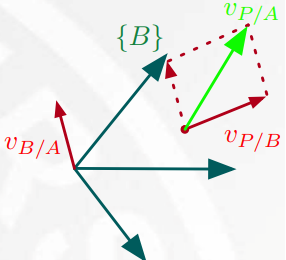
\includegraphics[width=.35\textwidth]{Linear Velocity}} \quad
\subfloat[旋转]{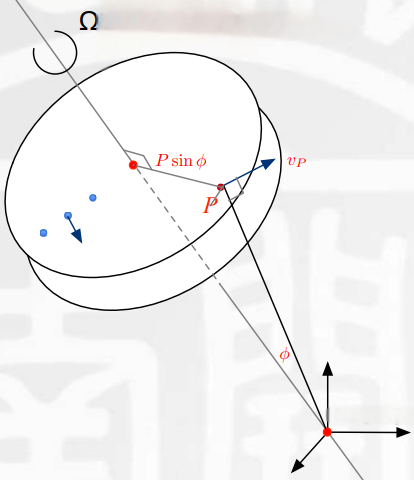
\includegraphics[width=.3\textwidth]{Rotational Motion}}
\caption{速度合成}
\end{figure}

\begin{itemize}
\item 相对速度:平行四边形法则,$ v_{P/A} = v_{B/A} + v_{P/B} $,$ v_{i/j} $指$ i $相对于$ j $坐标系的速度。
\item 旋转:垂直于原平面,$ v_p = \Omega \times P $,注意先后顺序。
\item 综合:$ ^A v_{P/A} = ^A v_{B/A} + ^A_B R \cdot ^B v_{P/B} + ^A \Omega \times (^A_B R \cdot ^B P) $,注意统一坐标系。
\end{itemize}
%------------------------------------------------
\paragraph{课程内容}
\begin{figure}[H]
\centering
\subfloat[控制系统]{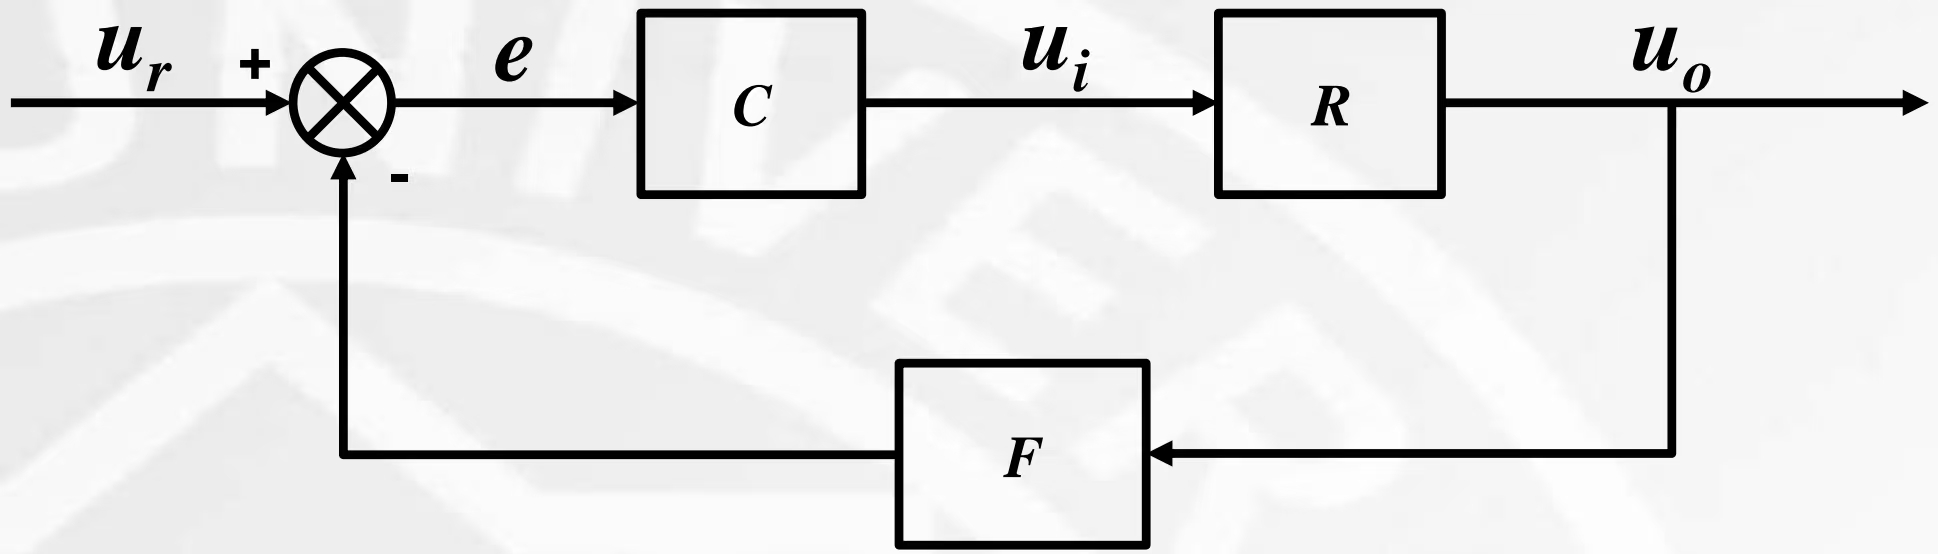
\includegraphics[width=.5\textwidth]{control}} \quad
\subfloat[正逆运动学]{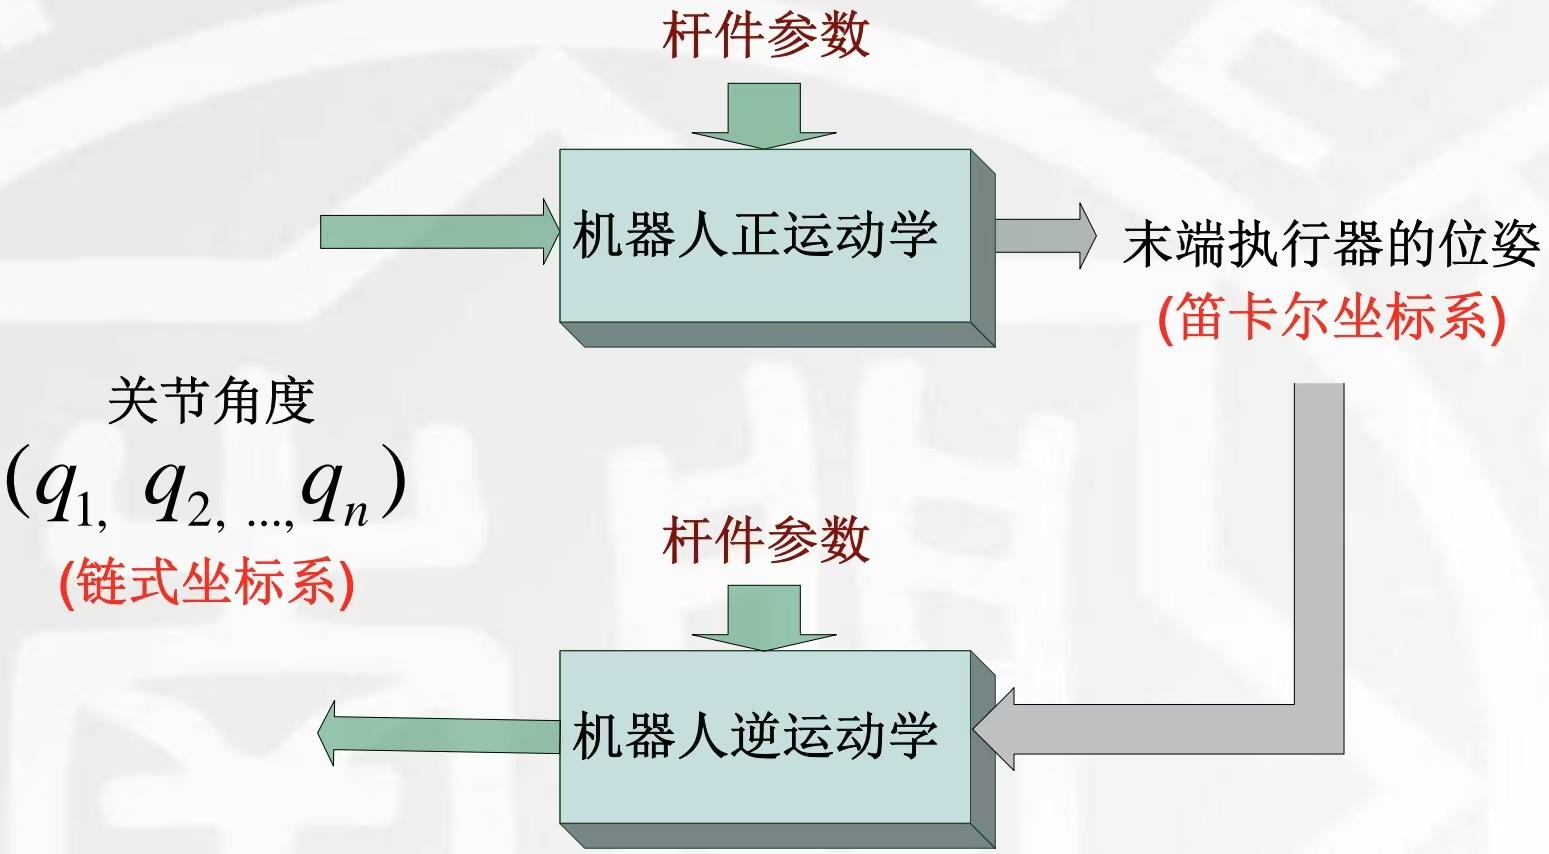
\includegraphics[width=.35\textwidth]{kinematics}}
\caption{课程内容}
\end{figure}

\begin{table}[H]
\centering
\begin{tabular}{|p{0.9cm}|p{2cm}|p{2cm}|p{2cm}|p{2cm}|p{2cm}|p{2cm}|p{2cm}|}
\hline
& $ u_i $ & $ u_o $ & $ R $ & $ F $ & $ u_r $ & $ e $ & $ C $ \\
\hline
概念 & 系统输入 & 系统输出 & 系统模型 & 反馈单元 & 系统给定 & 系统误差 & 控制器 \\
\hline
含义 & 对被控对象施加作用的手段 & 可测目标状态 & 输入输出映射 & 输出映射变换 & 目标 & 目标与测量状态差值 & 误差与输入映射 \\
\hline
内容 & \multicolumn{2}{l|}{空间描述与变换} & \multicolumn{2}{p{4cm}|}{正、逆运动学,雅可比,动力学} & 轨迹规划 & \multicolumn{2}{l|}{机器人控制} \\
\hline
\end{tabular}
\caption{课程内容}
\end{table}

\begin{itemize}
\item 正运动学($ f:q \rightarrow {}^B E $):已知关节角度和位置,计算末端执行器位姿。
\item 逆运动学($ f:\{{}^B E\} \rightarrow q $):给定末端执行器位姿,求各关节需达到的角度和位置。
\end{itemize}
%----------------------------------------------------------------------------------------
\section{空间描述与变换}
%------------------------------------------------
\subsection[空间描述]{空间描述}
%------------------------------------------------
\subsubsection[坐标系]{坐标系}
\begin{itemize}
\item 笛卡尔坐标系$ (x, y, z) $:标准正交基,右手法则。
\item 圆柱坐标系$ (r, \theta, \mu) $:
$ 
\begin{cases}
x = r \cos\theta &r \geq 0 \\
y = r \sin\theta &0 \leq \theta \leq 2 \pi \\
z = \mu
\end{cases} 
$。
\item 球坐标系$ (r, \alpha, \beta) $:
$ 
\begin{cases}
x = r \cos\beta \cos\alpha &r \geq 0 \\
y = r \cos\beta \sin\alpha &0 \leq \alpha \leq 2\pi \\
z = r \sin\beta &0 \leq \beta \leq 2\pi
\end{cases} 
$。
\end{itemize}

\begin{figure}[H]
\centering
\subfloat[笛卡尔坐标系]{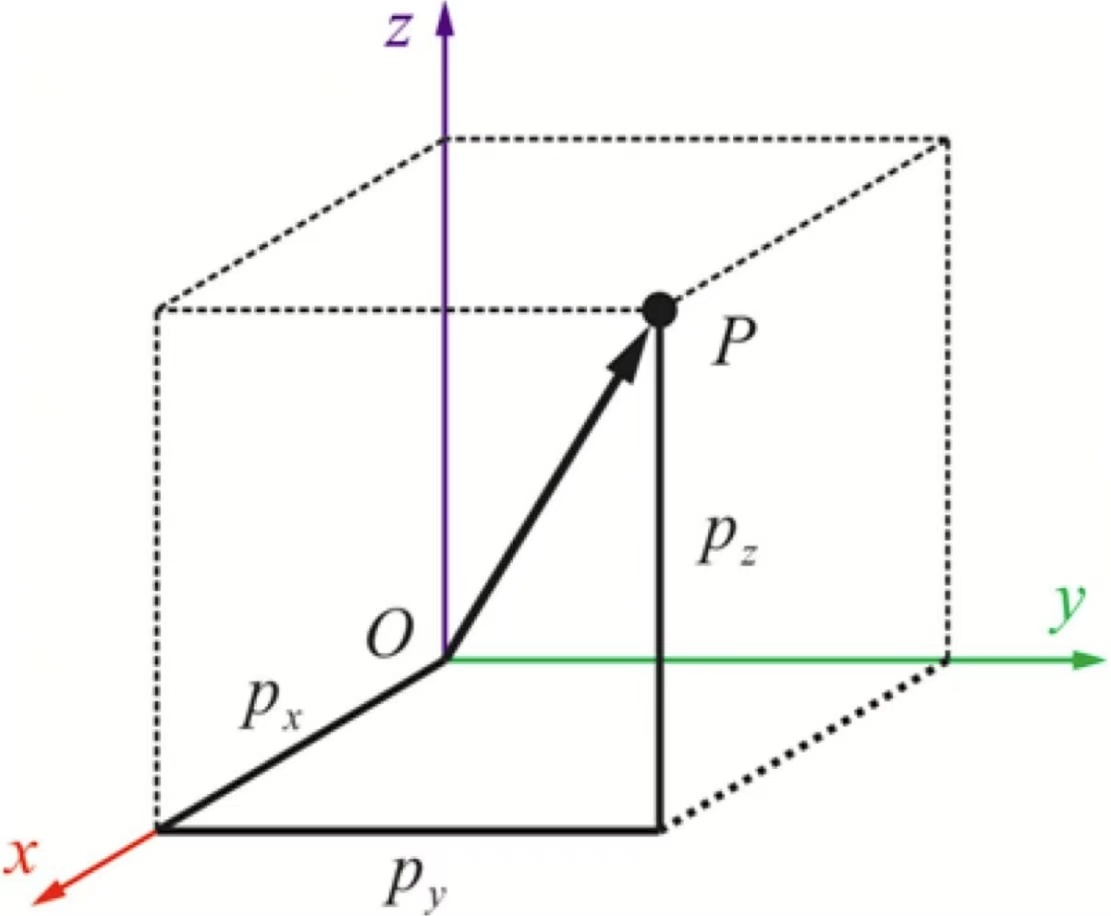
\includegraphics[width=.25\textwidth]{Cartesian}} \quad
\subfloat[圆柱坐标系]{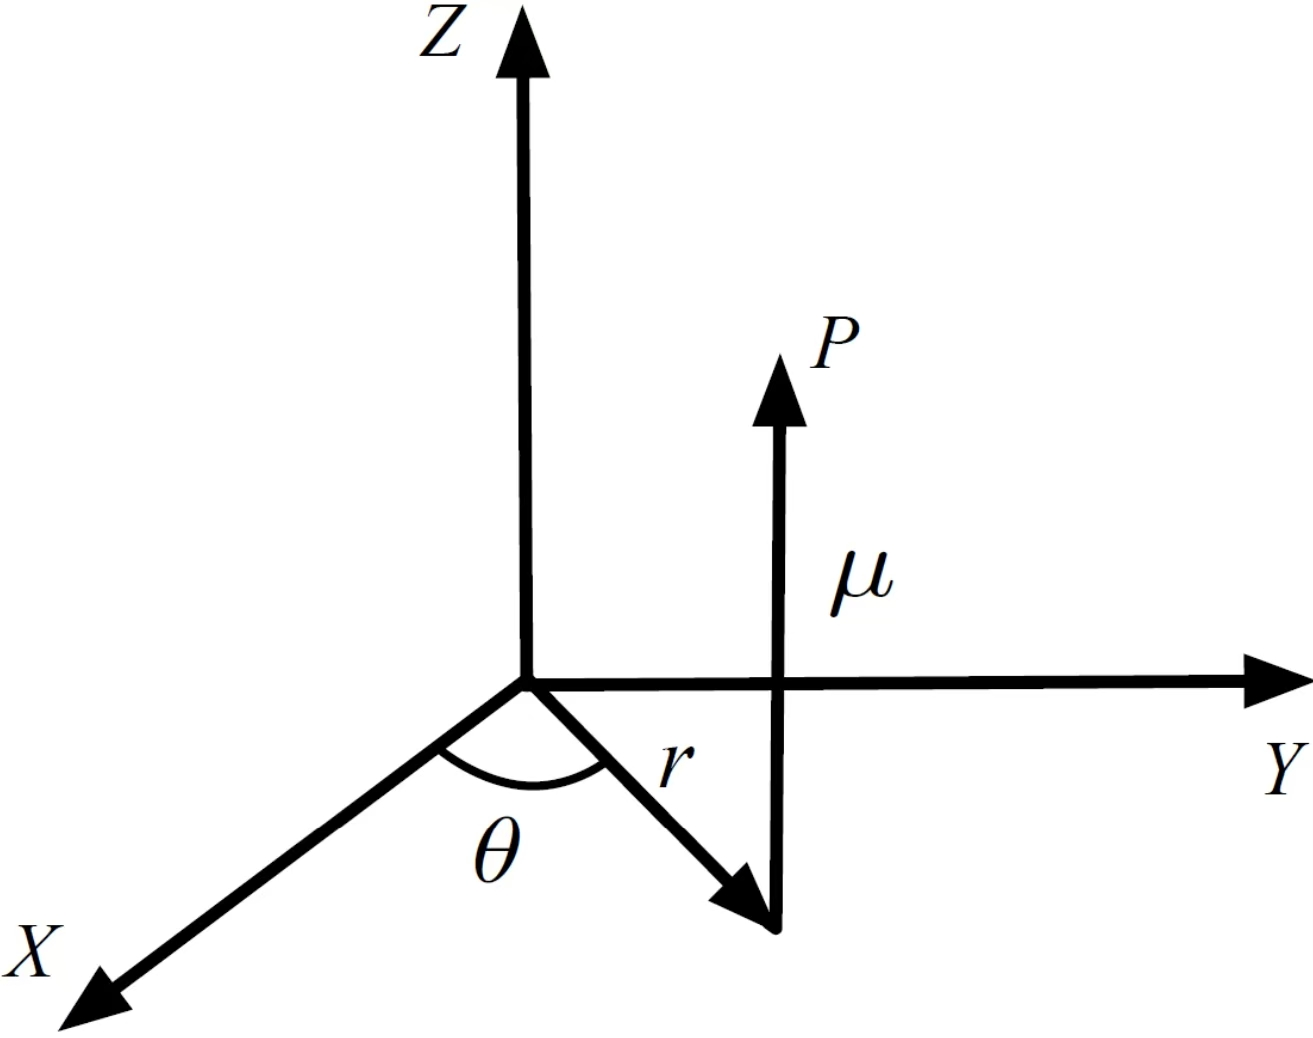
\includegraphics[width=.25\textwidth]{cylindrical}} \quad
\subfloat[球坐标系]{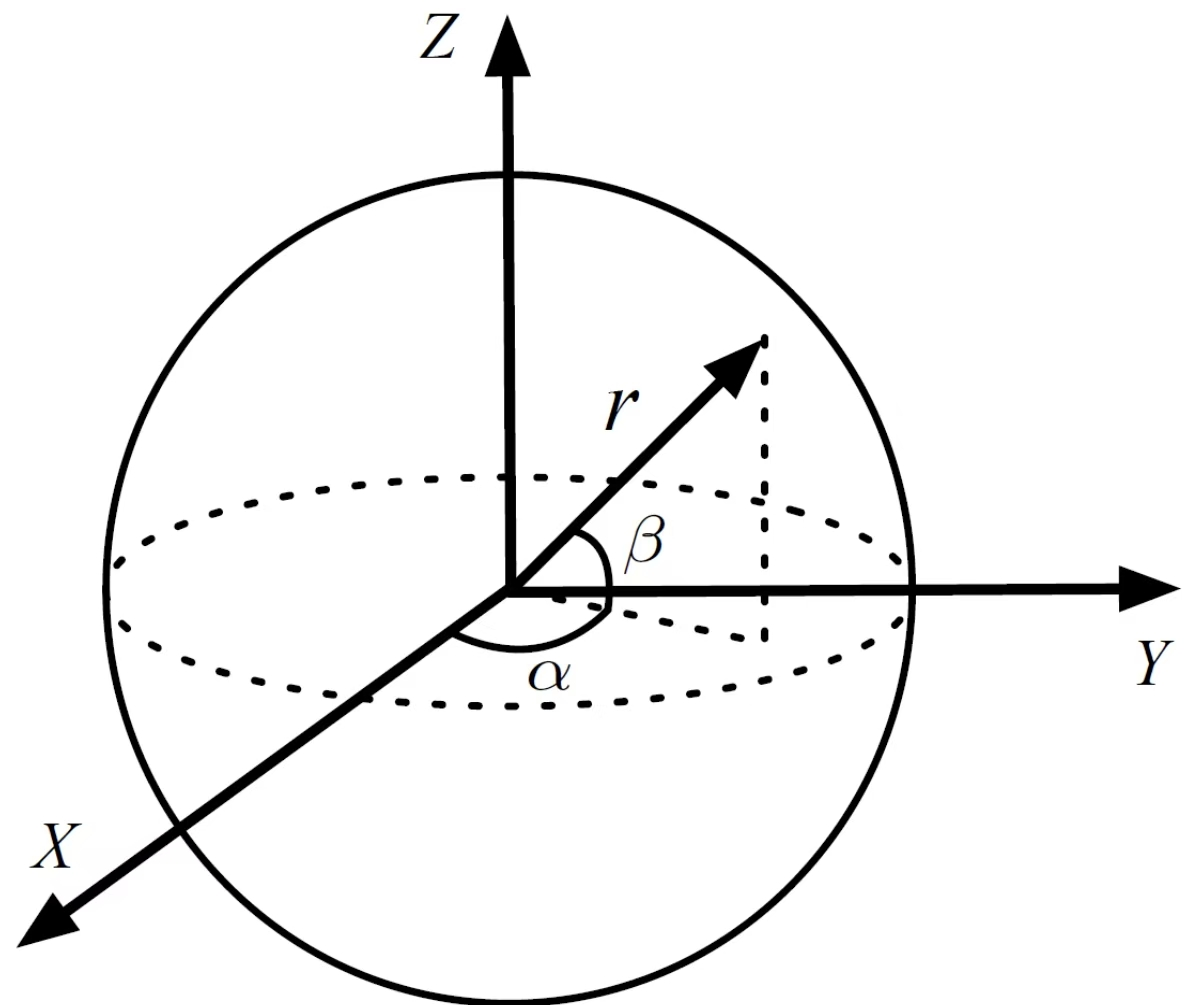
\includegraphics[width=.25\textwidth]{Spherical}}
\caption{坐标系}
\end{figure}
%------------------------------------------------
\subsubsection[刚体]{刚体}
\noindent
\begin{minipage}{0.7\textwidth}
\begin{itemize}
\item 刚体上任意两点间相对距离保持不变,角(加)速度相同。
\item 空间描述:位姿(Pose)=位置(Position)$ P_{Borg} $ + 姿态(Orientation)$ \{\vec x_B, \vec y_B, \vec z_B\} $。
\item 自由刚体空间运动:6个自由度,沿$ x, y, z $轴的平移和旋转。
\end{itemize}
\end{minipage}
\begin{minipage}{0.3\textwidth}
\begin{figure}[H]
\centering 
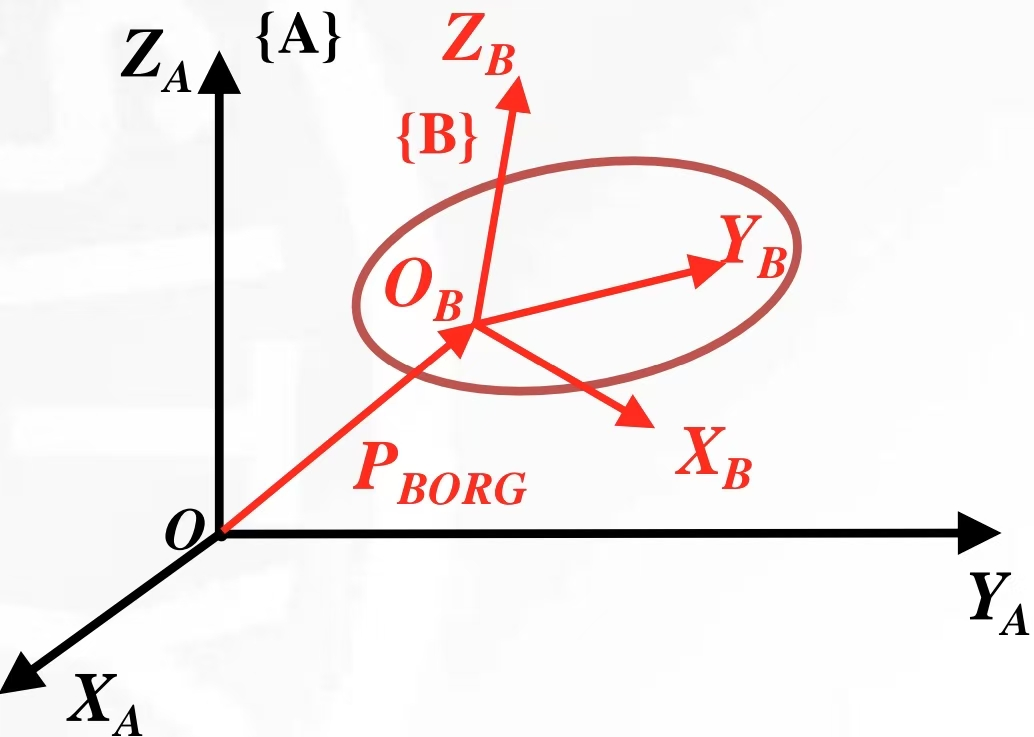
\includegraphics[width=0.8\textwidth]{rigid} 
\caption{刚体位姿}
\end{figure}
\end{minipage}
%------------------------------------------------
\subsection[变换]{变换}
%------------------------------------------------
\subsubsection[变换阵]{变换阵($ {}^A X = {}^A_B R/T \cdot {}^B X $)\tip{变换阵(逆变换、复合变换)}}
%------------------------------------------------
\paragraph{旋转阵(Rotation Matrix)}
$$ 
{}^A_B R 
= \begin{bmatrix} r_{11} & r_{12} & r_{13} \\ r_{21} & r_{22} & r_{23} \\ r_{31} & r_{32} & r_{33} \end{bmatrix}_{3 \times 3}
= \begin{bmatrix} {}^A \vec{x}_B & {}^A \vec{y}_B & {}^A \vec{z}_B \end{bmatrix}
= \begin{bmatrix} {}^B \vec{x}_A^T \\ {}^B \vec{y}_A^T \\ {}^B \vec{z}_A^T \end{bmatrix}
= \begin{bmatrix} X_B X_A & Y_B X_A & Z_B X_A \\ X_B Y_A & Y_B Y_A & Z_B Y_A \\ X_B Z_A & Y_B Z_A & Z_B Z_A \end{bmatrix}
$$
\begin{itemize}
\item 单位正交阵$ {}^A_B R $满秩。
\item 求解:每列是B的基在A下的表示,每行是A的基在B下的表示。
\item $ {}^A_B R^{-1} = {}^A_B R^T = {}^B_A R $。
\end{itemize}
%------------------------------------------------
\paragraph{齐次变换阵}
$$ {}^A_B T = \begin{bmatrix} {}^A_B R & {}^A P_{Borg} \\ \underbrace{0}_{\text{透视变换}} & \underbrace{1}_{\text{比例}} \end{bmatrix}_{4 \times 4} $$
\begin{itemize}
\item $ {}^A_B T $满秩。
\item 求解:求$ {}^A_B R $,填底行,求$ P_{Borg} $(沿$ A $坐标系,即旋转完的$ B $坐标系,$ B $到$ A $的移动)。
\item 
$ 
{}^A_B T^{-1} = {}^B_A T 
= \begin{bmatrix} {}^B_A R & {}^B P_{Aorg} \\ 0 & 1 \end{bmatrix} 
= \begin{bmatrix} {}^A_B R^T & -{}^A_B R^T \cdot {}^A P_{Borg} \\ 0 & 1 \end{bmatrix} 
$,

推导:$ {}^B({}^A P_{Borg}) = {}^B_A R \cdot {}^A P_{Borg} + {}^B P_{Aorg} = 0 $。
\end{itemize}
%------------------------------------------------
\paragraph{复合变换}
\begin{itemize}
\item $ {}^A_C T = {}^A_B T \cdot {}^B_C T $:左下消右上,链式。
\item 计算顺序与计算量:$ {}^A P = {}^A_B T \cdot {}^B_C T \cdot {}^C P $,从左向右先推导旋转阵比从右向左依次变换计算量大很多。
\end{itemize}
%------------------------------------------------
\subsubsection[映射与算子]{映射与算子\tip{映射与算子}}
\begin{itemize}
\item 坐标系映射(Mapping)——不同坐标系$ B \rightarrow A $,右乘
$$ {}^A P = \underbrace{{}^A_B R \cdot {}^B P}_{\text{旋转}} + \underbrace{{}^A P_{Borg}}_{\text{平移}} = {}^A_B T \cdot {}^B P $$

\hspace{2em}
分开计算旋转和平移时,一般先旋转后平移(不同坐标系的矢量只有在坐标系姿态相同时才可以加减)。
\item 向量变换算子(Operator)——同一坐标系$ P_1 \rightarrow P_2 $,左乘
$$ {}^A P_2 = \underbrace{R_K(\theta) \cdot {}^A P_1}_{\text{旋转}} + \underbrace{{}^A Q}_{\text{平移}} = T \cdot {}^A P_1 $$
\item 旋转算子(绕$ k $转$ \theta $角,右手系正方向):
$$
R_x(\theta) = \begin{bmatrix} 1 & 0 & 0 \\ 0 & \cos\theta & -\sin\theta \\ 0 & \sin\theta & \cos\theta \end{bmatrix}, 
R_y(\theta) = \begin{bmatrix} \cos\theta & 0 & \sin\theta \\ 0 & 1 & 0 \\ -\sin\theta & 0 & \cos\theta \end{bmatrix}, 
R_z(\theta) = \begin{bmatrix} \cos\theta & -\sin\theta & 0 \\ \sin\theta & \cos\theta & 0 \\ 0 & 0 & 1 \end{bmatrix}
$$
\end{itemize}
\begin{minipage}{0.6\textwidth}
\begin{figure}[H]
\centering
\subfloat[旋转映射]{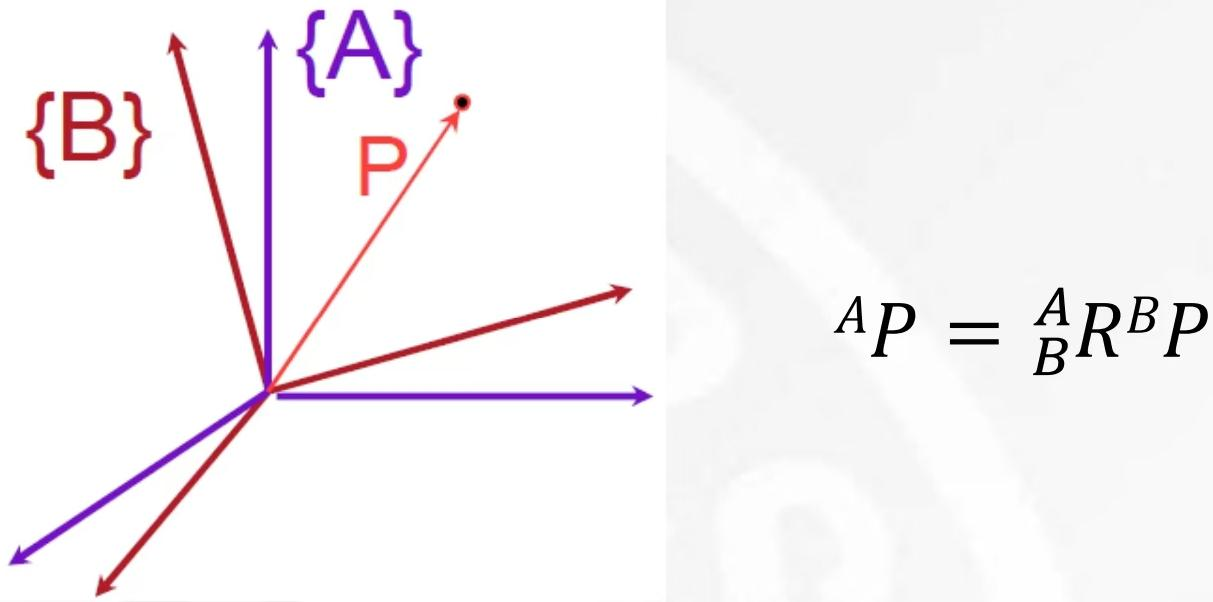
\includegraphics[width=.45\textwidth]{Mapping_r}} \quad
\subfloat[旋转算子]{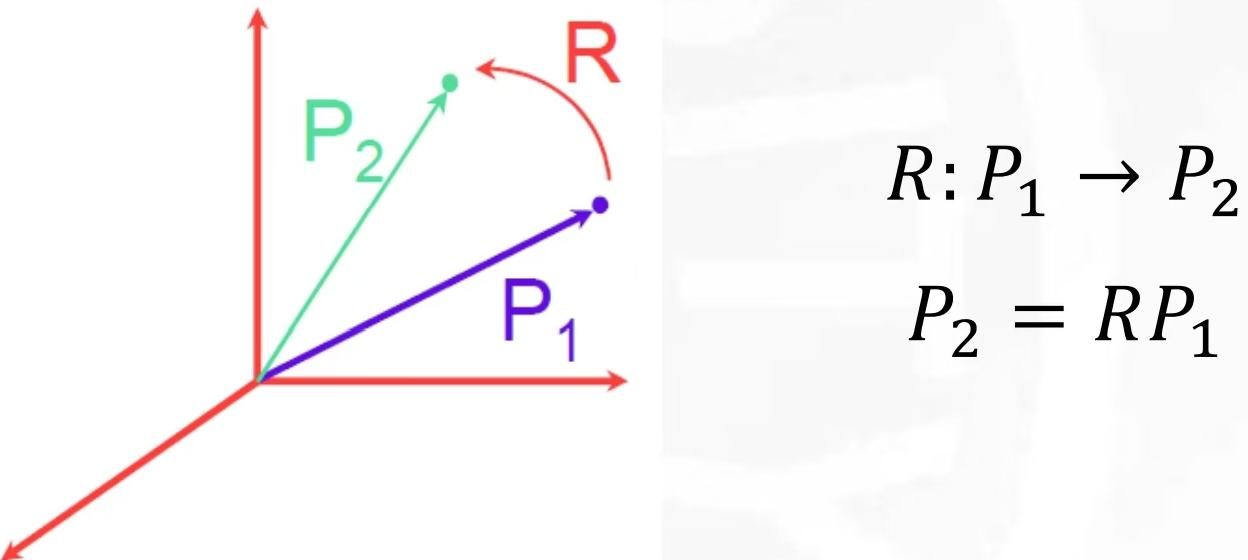
\includegraphics[width=.45\textwidth]{Operator_r}}\\
\subfloat[平移映射]{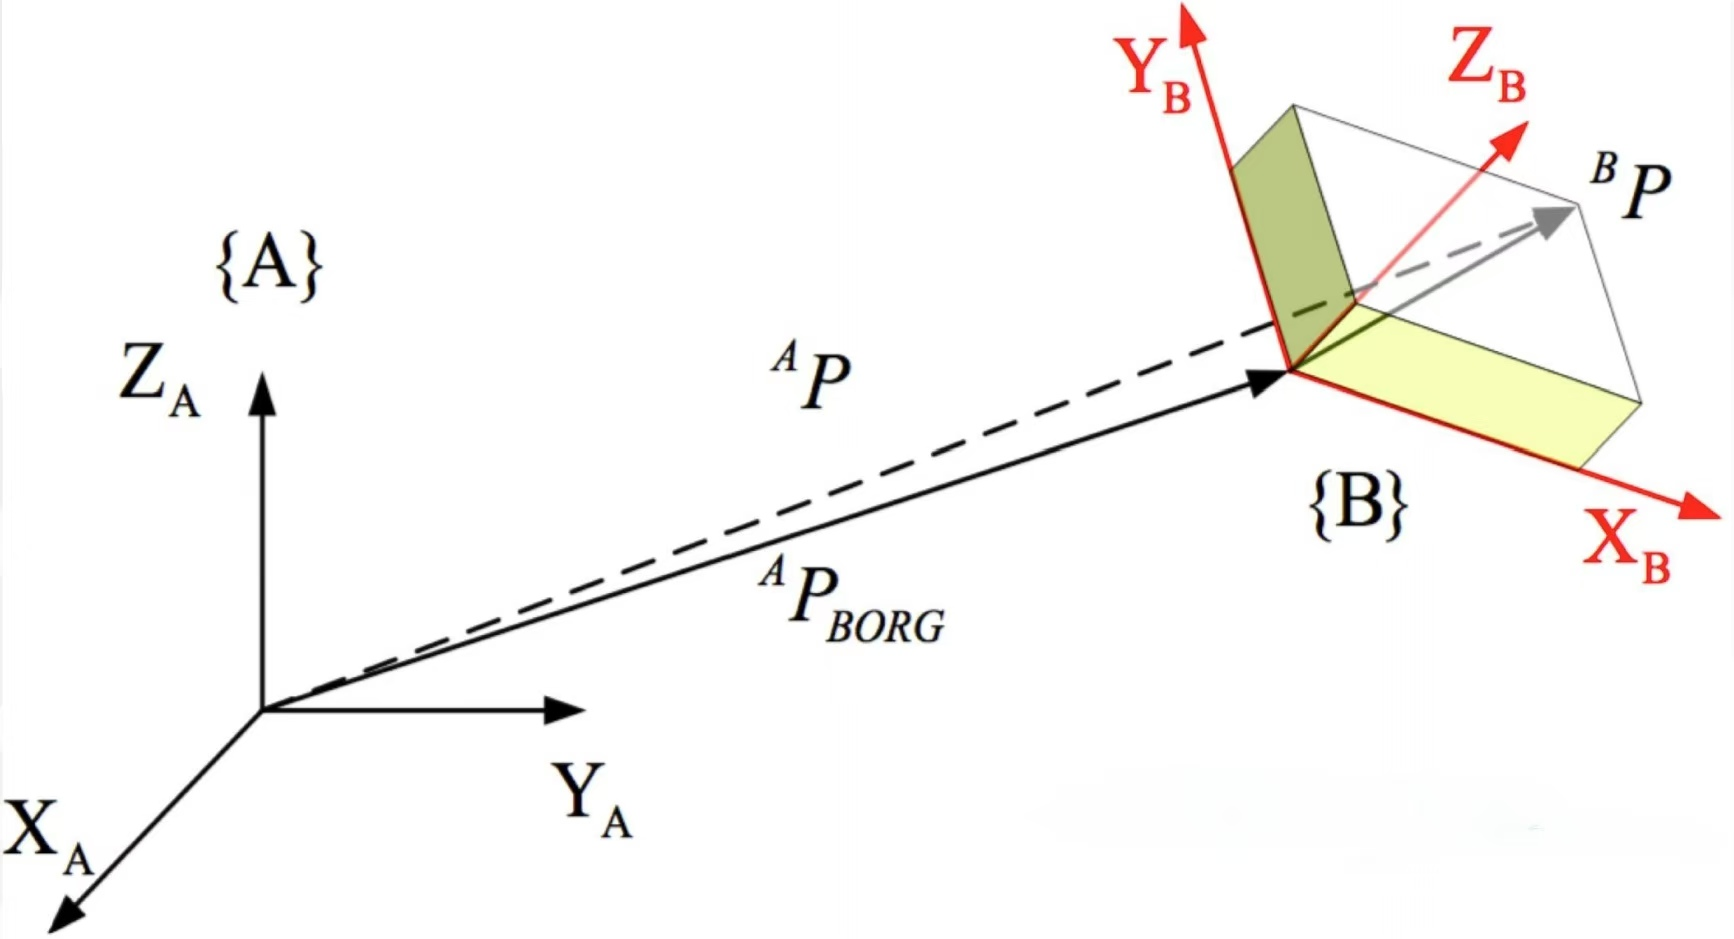
\includegraphics[width=.45\textwidth]{Mapping_p}} \quad
\subfloat[平移算子]{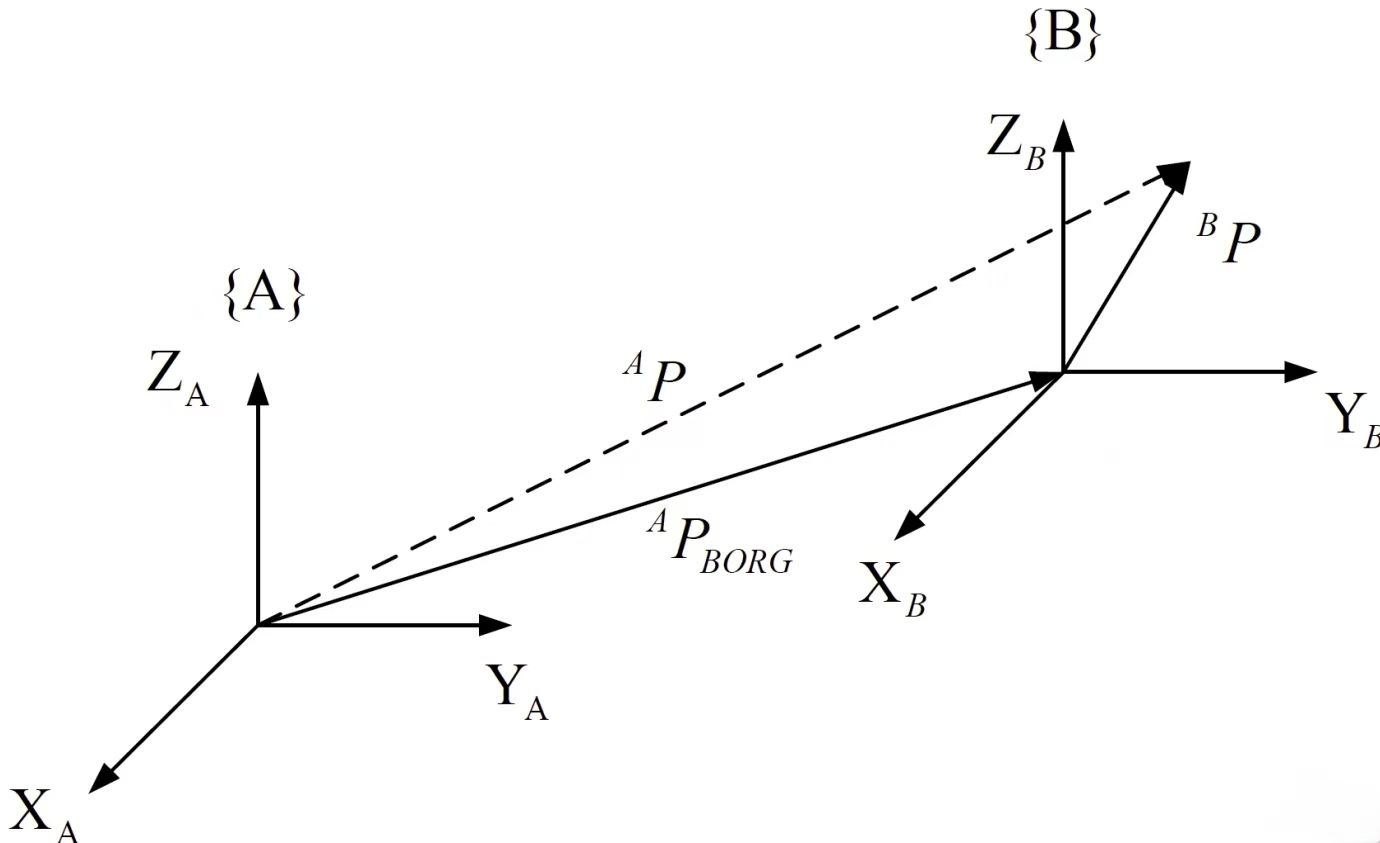
\includegraphics[width=.45\textwidth]{Operator_p}}
\caption{映射与算子对比}
\end{figure}
\end{minipage}
\begin{minipage}{0.4\textwidth}
\begin{table}[H]
\centering
\begin{tabular}{c|cc}
\hline
& 映射 & 算子 \\
\hline
坐标系 & 不同 & 同一 \\
连乘 & 右乘 & 左乘 \\
\hline
\end{tabular}
\caption{映射与算子对比}
\end{table}
\end{minipage}
%------------------------------------------------
\subsection[姿态描述]{姿态描述}
%------------------------------------------------
\subsubsection[描述方式]{描述方式\tip{姿态描述方式}}
%------------------------------------------------
\paragraph{旋转矩阵与方向余弦}
\begin{itemize}
\item 旋转矩阵$ R = \begin{bmatrix} r_{11} & r_{12} & r_{13} \\ r_{21} & r_{22} & r_{23} \\ r_{31} & r_{32} & r_{33} \end{bmatrix} $$ \Leftrightarrow $方向余弦$ x_r = \begin{bmatrix} {r_1}_{(3 \times 1)} \\ {r_2}_{(3 \times 1)} \\ {r_3}_{(3 \times 1)} \end{bmatrix}_{(9 \times 1)} $。
\item $ 9 $个变量,$ 6 $个约束(单位 + 正交),$ 3 $个独立变量。
\end{itemize}
%------------------------------------------------
\paragraph{等效轴角(绕空间中一轴旋转)}
\begin{itemize}
\item 坐标轴$ B $绕$ {}^A \hat{k} = \begin{bmatrix} k_x & k_y & k_z \end{bmatrix}^T (k_x^2 + k_y^2 + k_z^2 = 1) $旋转$ \theta $角,先使坐标轴$ B $与坐标轴$ A $重合,再使一轴(以下以$ z $轴为例)与$ ^A \hat{k} $重合,最后绕重合轴旋转$ \theta $角。
\begin{align*}
R(\theta, {}^A \hat{k}) &= R_K(\theta) = R_z(\alpha) \cdot R_y(\beta) \cdot R_z(\theta) \cdot R_y^T(\beta) \cdot R_z^T(\alpha) \\
&= \begin{bmatrix} k_x k_x v\theta + c\theta & k_x k_y v\theta - k_z s\theta & k_x k_z v\theta + k_y c\theta \\ k_x k_y v\theta + k_z s\theta & k_y k_y v\theta + c\theta & k_y k_z v\theta - k_x s\theta \\ k_x k_z v\theta - k_y c\theta & k_y k_z v\theta + k_x s\theta & k_z k_z v\theta + c\theta \end{bmatrix} 
\end{align*}

其中$ c\theta = \cos\theta, s\theta = \sin\theta, v\theta = 1 - \cos\theta $。
\item 与旋转矩阵结合:
$$ \theta = \arccos(\frac{r_{11} + r_{22} + r_{33} - 1}{2}), {}^A \hat{k} = \frac{1}{2 \sin\theta} \begin{bmatrix} r_{32} - r_{23} & r_{13} - r_{31} & r_{21} - r_{12} \end{bmatrix}^T $$
\begin{itemize}
\item 多解:$ \arccos $多解。    
\item 奇异:$ \sin\theta = 0 $。
\end{itemize}
\end{itemize}
%------------------------------------------------
\paragraph{四元数(欧拉参数)}~\\

由轴$ \hat{k} = \begin{bmatrix} k_x & k_y & k_z \end{bmatrix}^T (k_x^2 + k_y^2 + k_z^2 = 1) $和$ \theta $,得到欧拉参数:
$$ \varepsilon_1 = k_x \sin\frac{\theta}{2}, \varepsilon_2 = k_y \sin\frac{\theta}{2}, \varepsilon_3 = k_z \sin\frac{\theta}{2}, \varepsilon_4 = \cos\frac{\theta}{2} $$

有$ \varepsilon_1^2 + \varepsilon_2^2 + \varepsilon_3^2 + \varepsilon_4^2 = 1 $,其表示超球体上一点,至少有一个参数不小于$ \frac{1}{2} $。

表示为旋转阵$ R = \begin{bmatrix} 1 - 2(\varepsilon_2^2 + \varepsilon_3^2) & 2(\varepsilon_1 \varepsilon_2 - \varepsilon_3 \varepsilon_4) & 2(\varepsilon_1 \varepsilon_3 + \varepsilon_2 \varepsilon_4) \\ 2(\varepsilon_1 \varepsilon_2 + \varepsilon_3 \varepsilon_4) & 1 - 2(\varepsilon_1^2 + \varepsilon_3^2) & 2(\varepsilon_2 \varepsilon_3 - \varepsilon_1 \varepsilon_4) \\ 2(\varepsilon_1 \varepsilon_3 - \varepsilon_2 \varepsilon_4) & 2(\varepsilon_2 \varepsilon_3 + \varepsilon_1 \varepsilon_4) & 1 - 2(\varepsilon_1^2 + \varepsilon_2^2) \end{bmatrix} $

求解时,先计算$ \max{\varepsilon_i }$,用其计算其它参数,以保证最高精度。以下以$ \varepsilon_4 $为例:
\begin{itemize}
\item $ tr(R) = r_{11} + r_{22} + r_{33} = 3 - 4(\varepsilon_1^2 + \varepsilon_2^2 + \varepsilon_3^2) = 3 - 4(1 - \varepsilon_4^2) $。
\item $ \varepsilon_4 = \frac{1}{2} \sqrt{1 + r_{11} + r_{22} + r_{33}}, \varepsilon_1 = \frac{r_{32} - r_{23}}{4 \varepsilon_4}, \varepsilon_2 = \frac{r_{13} - r_{31}}{4 \varepsilon_4}, \varepsilon_3 = \frac{r_{21} - r_{12}}{4 \varepsilon_4} $。
\end{itemize}
%------------------------------------------------
\subsubsection[旋转角]{旋转角}
\begin{itemize}
\item 固定角(12种):绕同一坐标轴旋转,算子左乘。
\item 变角(12种):绕变换坐标轴旋转,映射右乘。
\begin{itemize}
\item 泰特布莱恩角:三个旋转轴不同,$ Z-Y-X $泰特布莱恩角与$ X-Y-Z $欧拉角对偶。
\item 欧拉角:第一个旋转轴与最后一个旋转轴相同,奇异现象(中间旋转导致前后旋转轴重合,自由度丢失)。
\end{itemize}
\end{itemize}
%----------------------------------------------------------------------------------------
\section{正运动学}
%------------------------------------------------
\subsection[机器人结构与自由度]{机器人结构与自由度}
\begin{itemize}
\item 运动副(Kinematic pairs):构件间连接结构,使构件只能相对运动(受约束),自由度减少。
\begin{itemize}
\item 接触方式:
\begin{itemize}
\item 低副:面接触,压强低。如旋转副、平移副。
\item 高副:点/线接触,压强高,易磨损。如凸轮副、齿轮副。
\end{itemize}
\item 根据引入的约束数目分类。
\item 转动副和移动副。
\end{itemize}
\item 关节(Joint):连接各构件的、能主动驱动产生相对运动的运动副,一个关节提供$ 5 $个约束和$ 1 $个自由度。
\begin{itemize}
\item 转动关节(Revolute joint)
\item 移动关节(Prismatic joint)
\end{itemize}
\item 连杆(Link):组成机器人的、由关节连接形成运动链的刚体,传递运动和力。
\begin{itemize}
\item 固定连杆(基座)
\item 运动连杆
\end{itemize}
\item 自由度=运动连杆数=关节数。
\item 冗余机器人:自由度大于$ 6 $的空间机器人和自由度大于$ 3 $的平面机器人。可以增加灵活性,避免奇异,提升避障能力,但因为逆运动学多解而求解复杂。
\end{itemize}
%------------------------------------------------
\subsection[DH参数]{DH参数}
%------------------------------------------------
\subsubsection[定义]{定义}
\begin{figure}[H]
\centering 
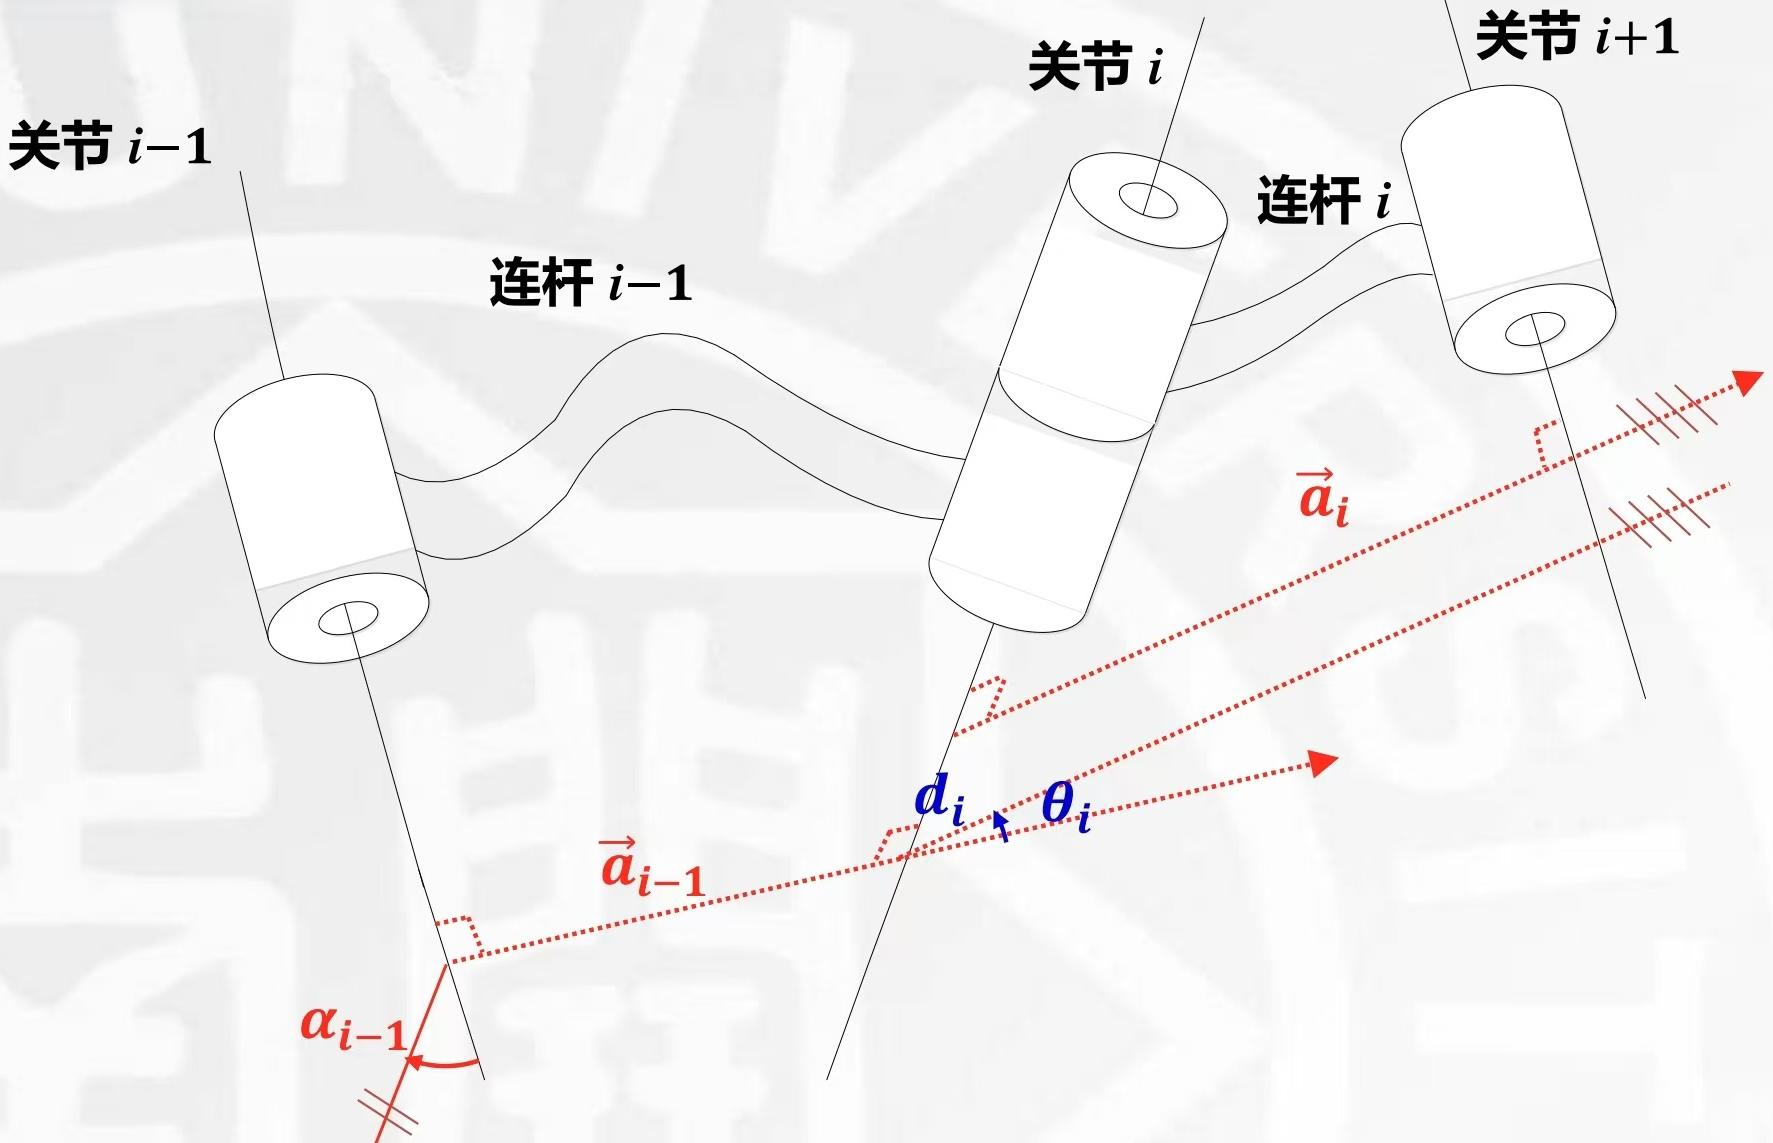
\includegraphics[width=0.5\textwidth]{dh} 
\caption{DH参数定义}
\end{figure}

对于关节$ i $:
\begin{itemize}
\item 连杆参数(几何参数):沿$ X_{i - 1} $,由$ Z_{i - 1} $与$ Z_i $求取,定值。
\begin{itemize}
\item 连杆长度(Link Length)$ \vec{a}_{i - 1}  $:公垂线段(除平行外唯一)长度。
\item 连杆扭角(Link Twist)$ \alpha_{i - 1} $:右手法则(指向末端)。
\end{itemize}
\item 关节参数(运动参数):沿$ Z_i $,由$ X_{i - 1} $与$ X_i $求取,平移关节$ \theta_i $为定值,旋转关节$ d_i $为定值,另一个为变量。
\begin{itemize}
\item 关节偏距(Joint Offset)$ d_i $:公垂线间距离。
\item 关节转角(Joint Angle)$ \theta_i $:公垂线夹角。
\end{itemize}
\item 
\begin{itemize}
\item 基座:虚拟关节$ 0 $与关节$ 1 $重合,$ \vec{a}_0 = 0, \alpha_0 = 0 $。
\item 末端:虚拟关节$ n + 1 $与关节$ n $重合,$ \vec{a}_n = 0, \alpha_n = 0 $。
\end{itemize}
\item 关节$ i $的DH参数表征其所在坐标系与前一坐标系的关系;坐标系$ i $的参数表征连杆$ i $沿其$ z $轴运动后相对于连杆$ i - 1 $的位姿。
\end{itemize}
\begin{minipage}{0.5\textwidth}
\begin{table}[H]
\centering
\begin{tabular}{c|cccc}
\hline
关节 & $ \alpha_{i - 1} $ & $ \vec{a}_{i - 1} $ & $ \theta_i $ & $ d_i $ \\
\hline
1 & $ 0 $ & $ 0 $ & $ \theta_1 $ & $ d_1 $ \\
2 & $ \alpha_1 $ & $ \vec a_1 $ & $ \theta_2 $ & $ d_2 $ \\
\hline
\end{tabular}
\caption{DH参数表}
\end{table}
\end{minipage}
\begin{minipage}{0.5\textwidth}
\begin{table}[H]
\centering
\begin{tabular}{c|cc}
\hline
相邻轴关系 & 角 & 距离 \\
\hline
共线 & $ 0 $ & $ 0 $ \\
平行 & $ 0 $ & $ d $ \\
相交 & $ \theta $ & $ 0 $ \\
不相交 & $ \theta $ & $ d $ \\
\hline
\end{tabular}
\caption{DH参数情况讨论}
\end{table}
\end{minipage}
%------------------------------------------------
\subsubsection[求解]{求解\tip{DH参数求解}}
\begin{enumerate}
\item $ Z_i $轴:关节$ i $轴延长线,标注正方向。
\item $ X_i $轴:$ Z_{i - 1} $轴与$ Z_i $轴公垂线(由前者指向后者)或交点(垂直平面,一般指向末端)。
\item ($ Y_i $轴:$ Z_i $轴与$ X_i $轴公垂线,右手法则确定。)
\item 标注基座坐标系和末端坐标系,尽可能与相邻坐标系重合。
\item 制表,并根据关节的平移或旋转属性在对应位置标注变量。
\item 沿$ X_{i - 1} $,由$ Z_{i - 1} $与$ Z_i $求取$ \vec{a}_{i - 1}  $和$ \alpha_{i - 1} $;沿$ Z_i $,由$ X_{i - 1} $与$ X_i $求取$ d_i $和$ \theta_i $。
\end{enumerate}
%------------------------------------------------
\subsubsection[例题]{例题\tip{DH参数例题}}
\begin{figure}[H]
\centering
\subfloat[例1结构图]{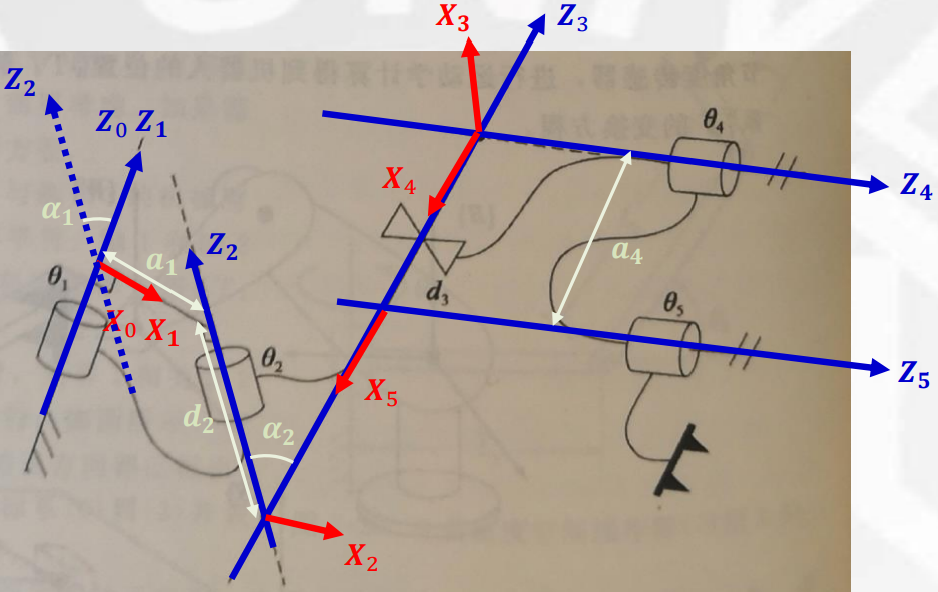
\includegraphics[width=.225\textwidth]{1.1.1}} \quad
\subfloat[例2结构图]{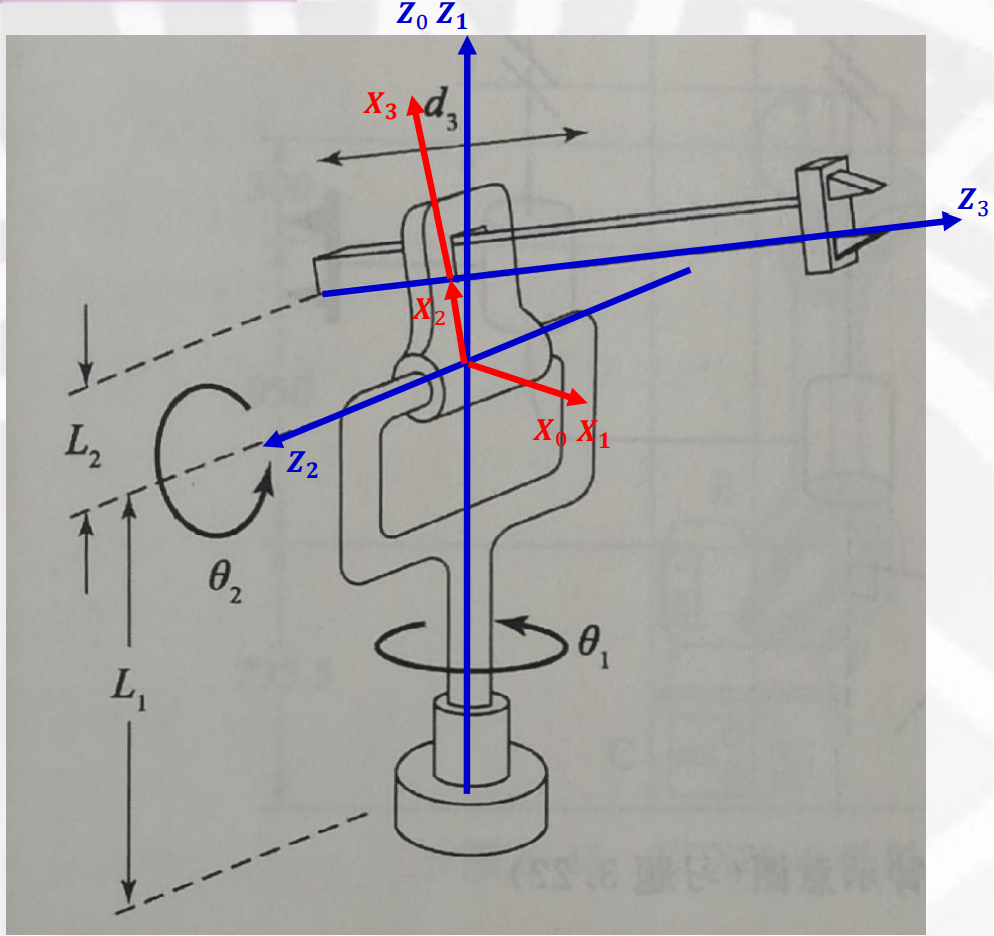
\includegraphics[width=.225\textwidth]{1.2.1}} \quad
\subfloat[例3结构图]{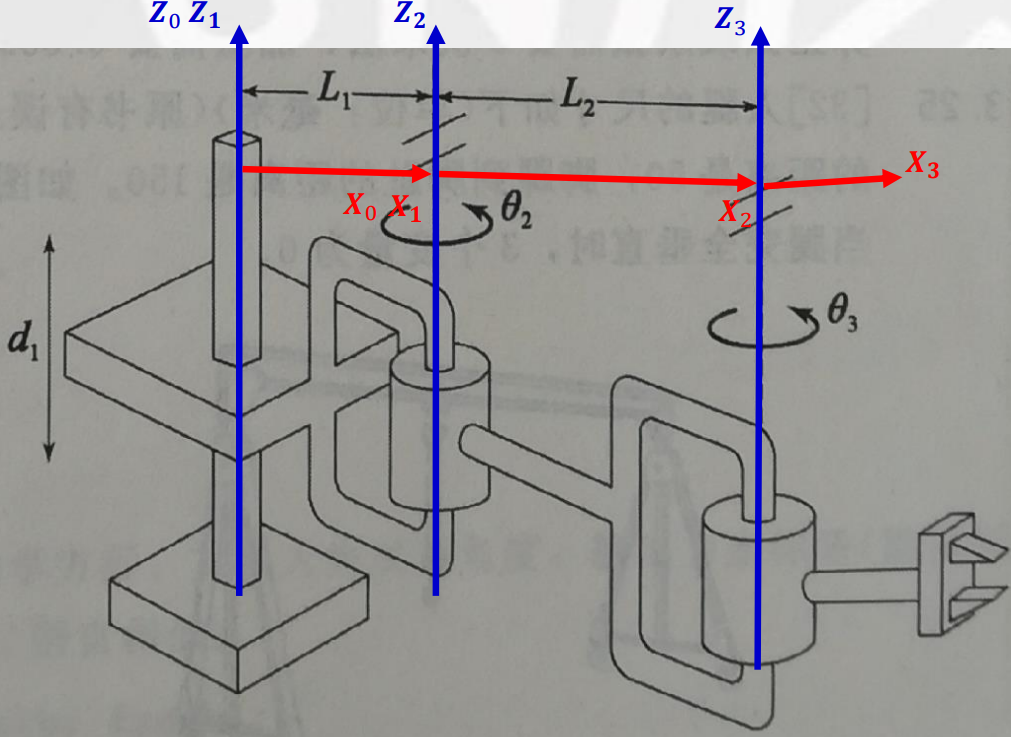
\includegraphics[width=.225\textwidth]{1.3.1}} \quad
\subfloat[例4结构图]{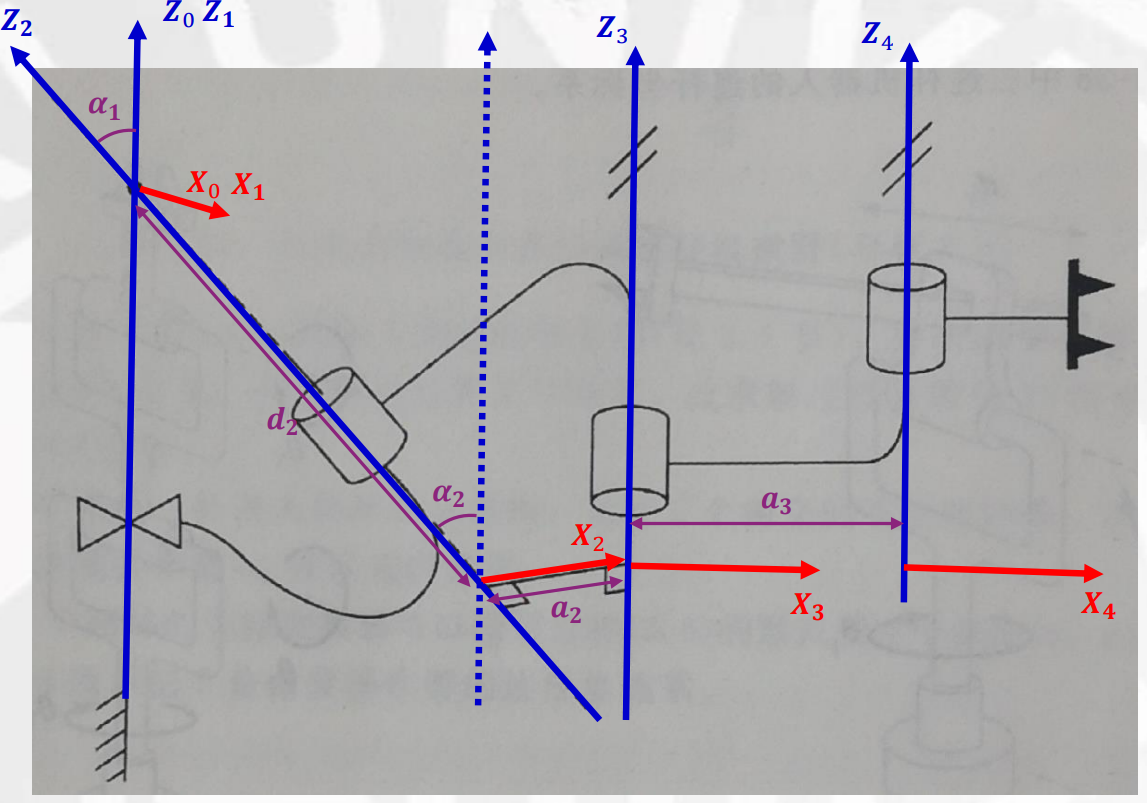
\includegraphics[width=.225\textwidth]{1.4.1}} \\
\subfloat[例1参数表]{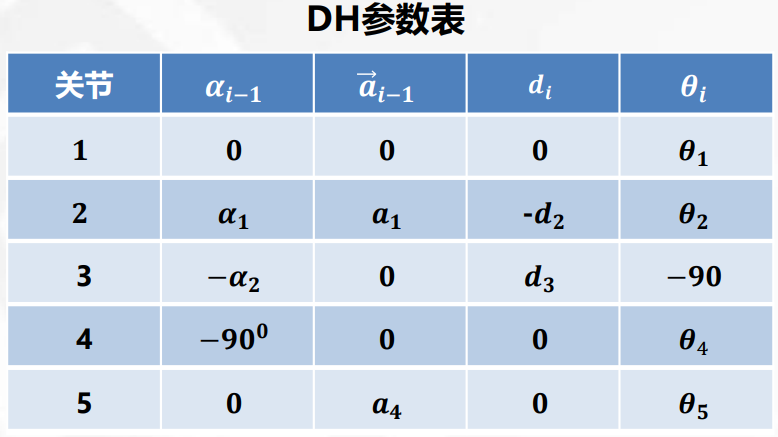
\includegraphics[width=.225\textwidth]{1.1.2}} \quad
\subfloat[例2参数表]{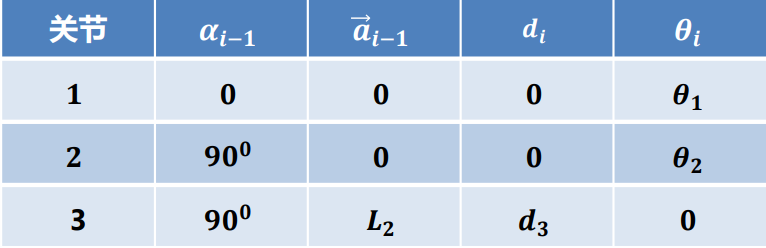
\includegraphics[width=.225\textwidth]{1.2.2}} \quad
\subfloat[例3参数表]{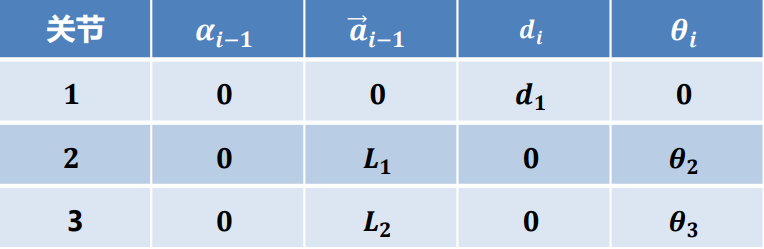
\includegraphics[width=.225\textwidth]{1.3.2}} \quad
\subfloat[例4参数表]{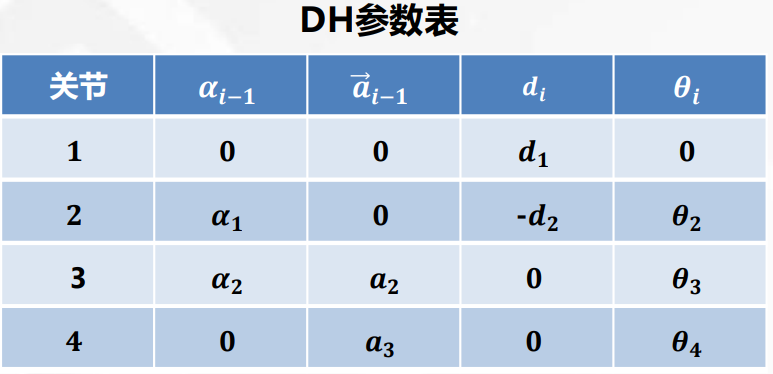
\includegraphics[width=.225\textwidth]{1.4.2}}
\caption{DH参数例题}
\end{figure}
%------------------------------------------------
\subsection[正运动学方程]{正运动学方程}
%------------------------------------------------
\subsubsection[求解]{求解\tip{正运动学方程求解}}
先根据连杆参数沿$ X $轴变换,再根据关节参数沿新$ Z $轴变换:
\begin{align*}
{}^{i - 1}_i T &= \begin{bmatrix} 1 & 0 & 0 & \vec{a}_{i - 1} \\ 0 & \cos\alpha_{i - 1} & -\sin\alpha_{i - 1} & 0 \\ 0 & \sin\alpha_{i - 1} & \cos\alpha_{i - 1} & 0 \\ 0 & 0 & 0 & 1 \end{bmatrix} \begin{bmatrix} \cos\theta_i & -\sin\theta_i & 0 & 0 \\ \sin\theta_i & \cos\theta_i & 0 & 0 \\ 0 & 0 & 1 & d_i \\ 0 & 0 & 0 & 1 \end{bmatrix} \\
&= \begin{bmatrix} \cos\theta_i & -\sin\theta_i & 0 & \vec{a}_{i - 1} \\ \sin\theta_i \cos\alpha_{i - 1} & \cos\theta_i \cos\alpha_{i - 1} & -\sin\alpha_{i - 1} & -d_i \sin\alpha_{i - 1} \\ \sin\theta_i \sin\alpha_{i - 1} & \cos\theta_i \sin\alpha_{i - 1} & \cos\alpha_{i - 1} & d_i \cos\alpha_{i - 1} \\ 0 & 0 & 0 & 1 \end{bmatrix}
\end{align*}

\begin{itemize}
\item 没有关于$ Y $轴的运动,静态的。
\item 按关节逐次变换,最终得到腕部坐标,而非末端坐标。
\end{itemize} 
%------------------------------------------------
\subsubsection[例题]{例题\tip{正运动学方程例题}}
\noindent
\begin{minipage}{0.45\textwidth}
\begin{figure}[H]
\centering
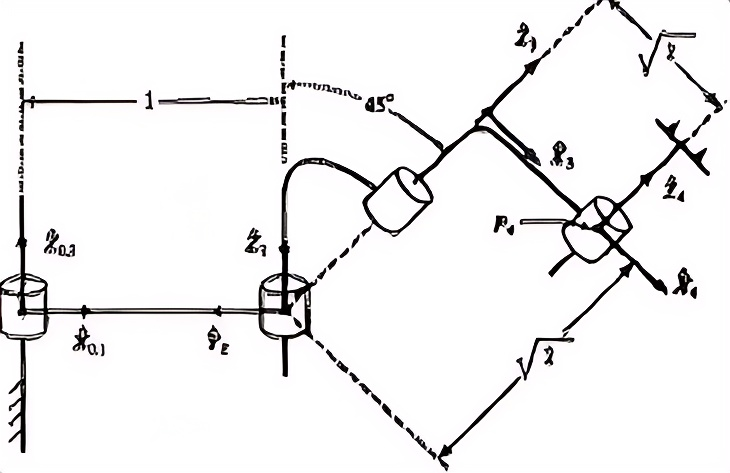
\includegraphics[width=\textwidth]{2.1}
\caption{正运动学方程例题}
\end{figure}
\end{minipage}
\begin{minipage}{0.55\textwidth}
\begin{table}[H]
\centering
\begin{tabular}{c|cccc}
\hline
$ i $ & $ \alpha_{i - 1} $ & $ a_{i - 1} $ & $ \theta_i $ & $ d_i $ \\
\hline
1 & $ 0 $ & $ 0 $ & $ \theta_1 $ & $ 0 $ \\
2 & $ 0 $ & $ 1 $ & $ \theta_2 $ & $ 0 $ \\
3 & $ \frac{\pi}{4} $ & $ 1 $ & $ \theta_3 $ & $ 0 $ \\
4 & $ 0 $ & $ \sqrt{2} $ & $ \theta_4 $ & $ 0 $ \\
\hline
\end{tabular}
\caption{正运动学方程例题DH参数表}
\end{table}
\end{minipage}
{\footnotesize
由其转化得到各齐次阵:
$$
{}^0_1T = \begin{bmatrix} c1 & -s1 & 0 & 0 \\ s1 & c1 & 0 & 0 \\ 0 & 0 & 1 & 0 \\ 0 & 0 & 0 & 1 \end{bmatrix},
{}^1_2T = \begin{bmatrix} c2 & -s2 & 0 & 1 \\ s2 & c2 & 0 & 0 \\ 0 & 0 & 1 & 0 \\ 0 & 0 & 0 & 1 \end{bmatrix},
{}^2_3T = \begin{bmatrix} c3 & -s3 & 0 & 0 \\ \frac{\sqrt{2}}{2}s3 & \frac{\sqrt{2}}{2}c3 & \frac{\sqrt{2}}{2} & 1 \\ -\frac{\sqrt{2}}{2}s3 & -\frac{\sqrt{2}}{2}c3 & \frac{\sqrt{2}}{2} & 1 \\ 0 & 0 & 0 & 1 \end{bmatrix},
{}^3_4T = \begin{bmatrix} c4 & -s4 & 0 & \sqrt{2} \\ s4 & c4 & 0 & 0 \\ 0 & 0 & 1 & 0 \\ 0 & 0 & 0 & 1 \end{bmatrix}
$$

最终得到正运动学方程:
$$ {}^0_4T = \begin{bmatrix} c12 c34 - \frac{\sqrt{2}}{2}s12 s34 & -c12 s34 - \frac{\sqrt{2}}{2}s12 c34 & -\frac{\sqrt{2}}{2}s12 & c1 + s12 + \sqrt{2}c12 c3 - s12 s3 \\ s12 c34 + \frac{\sqrt{2}}{2}c12 s34 & -s12 s34 + \frac{\sqrt{2}}{2}c12 c34 & \frac{\sqrt{2}}{2}c12 & s1 - c12 + \sqrt{2}s12 c3 + c12 s3 \\ \frac{\sqrt{2}}{2}s34 & \frac{\sqrt{2}}{2}c34 & \frac{\sqrt{2}}{2} & s3 + 1 \\ 0 & 0 & 0 & 1 \end{bmatrix} $$

续\ref{sec:example2.2},逆运动学求解。
}
%----------------------------------------------------------------------------------------
\section{逆运动学}
%------------------------------------------------
\subsection[逆运动学求解]{逆运动学求解}
由$ T = \begin{bmatrix} r_{11} & r_{12} & r_{13} & p_x \\ r_{21} & r_{22} & r_{23} & p_y \\ r_{31} & r_{32} & r_{33} & p_z \\ 0 & 0 & 0 & 1 \end{bmatrix} $求解关节角度。
%------------------------------------------------
\subsubsection[方法]{方法\tip{逆运动学求解}}
\begin{itemize}
\item 代数法:利用平方($ \sin^2x + \cos^2x = 1 $)、和差角公式等化简齐次变化阵求解。
\item 几何法:利用正余弦定理求解图形。
\item (数值法:迭代搜索求近似解。)
\end{itemize} 
%------------------------------------------------
\subsubsection[例题]{例题\tip{逆运动学例题}}
%------------------------------------------------
\paragraph{例题1}
\begin{figure}[H]
\centering
\subfloat[代数法]{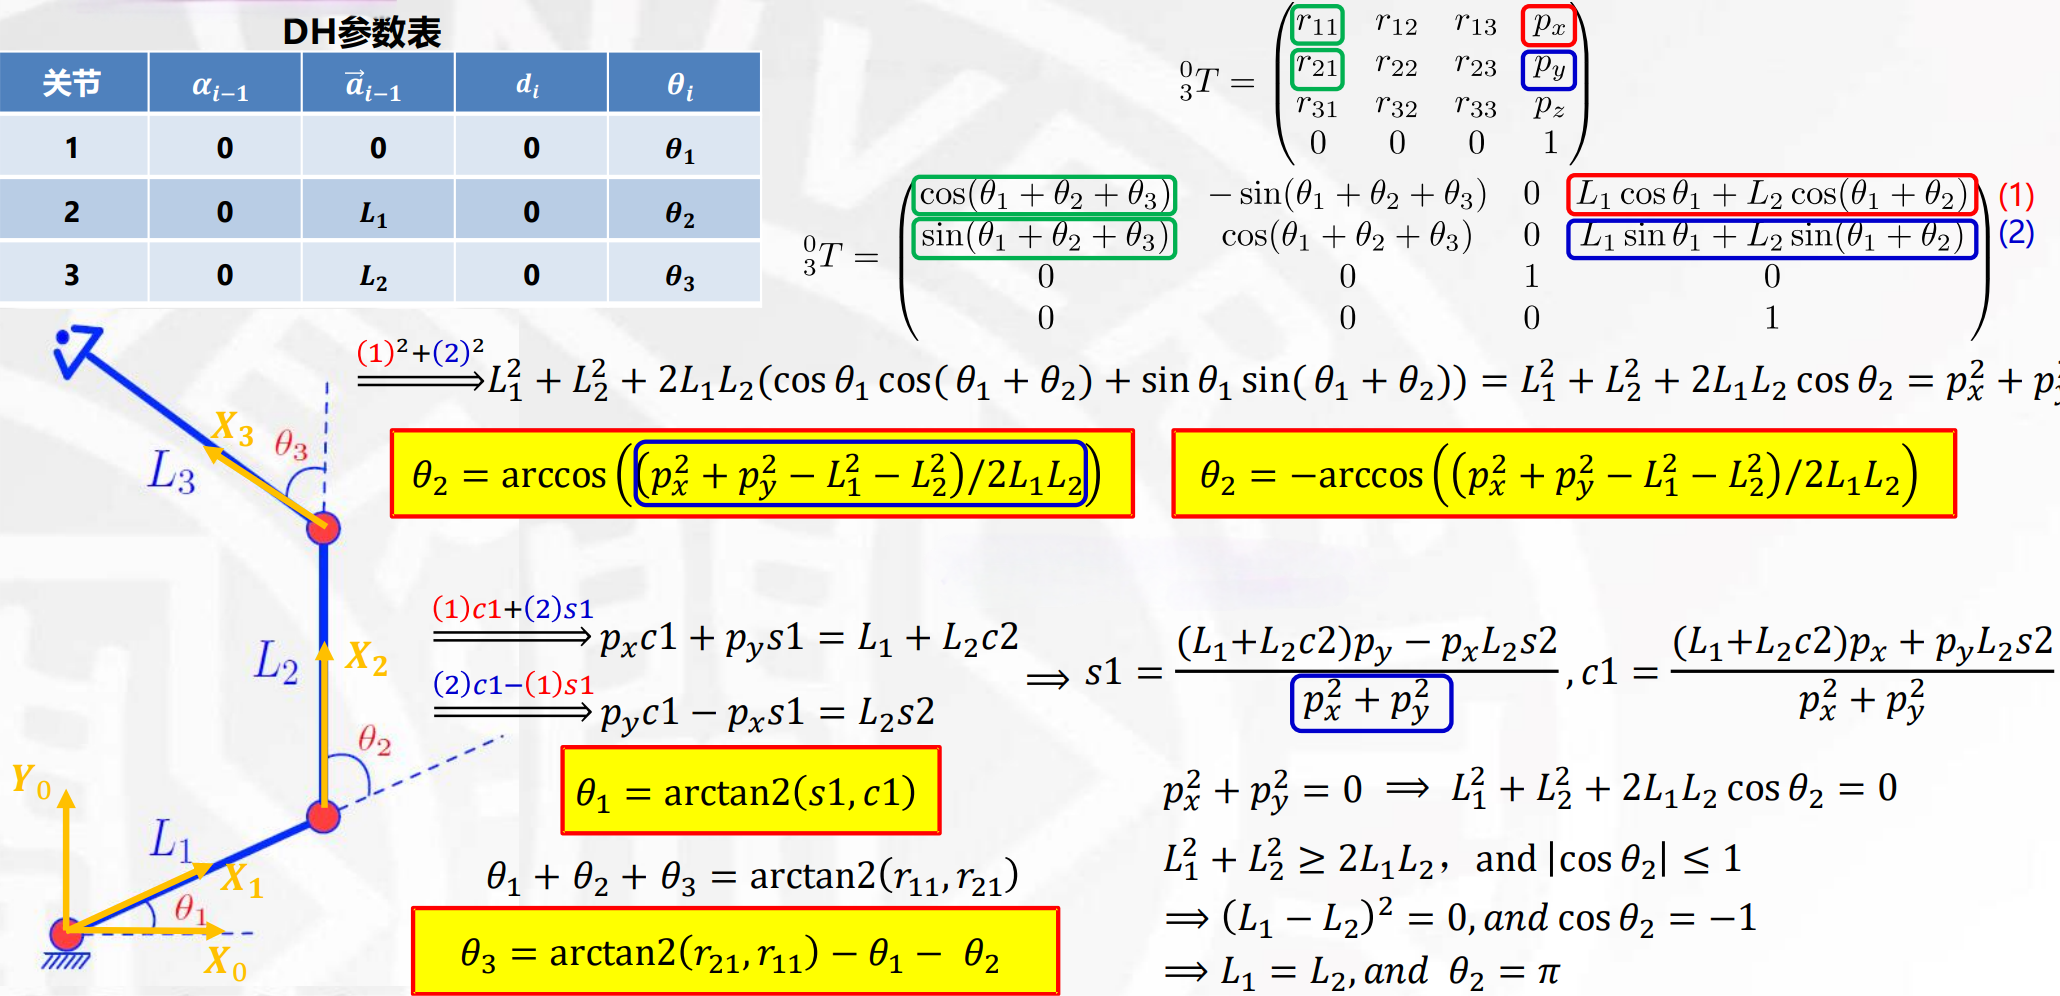
\includegraphics[width=0.7\textwidth]{3.1}} \\
\subfloat[几何法]{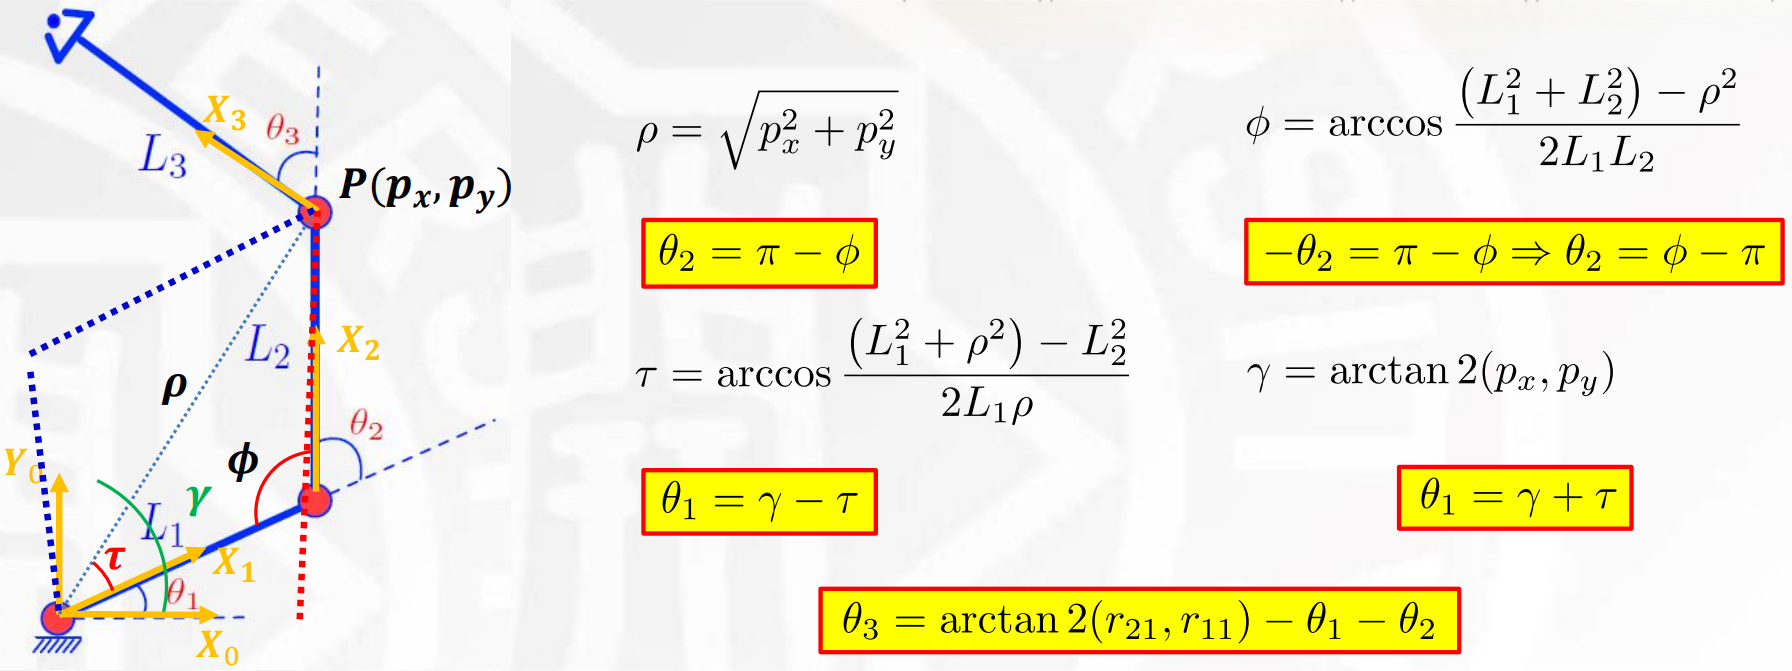
\includegraphics[width=0.6\textwidth]{3.2}}
\caption{逆运动学例题1}
\end{figure}
%------------------------------------------------
\paragraph{例题2}\label{sec:example2.2}
{\footnotesize 接\ref{sec:example2.1},使用代数法。}

\begin{figure}[H]
\centering 
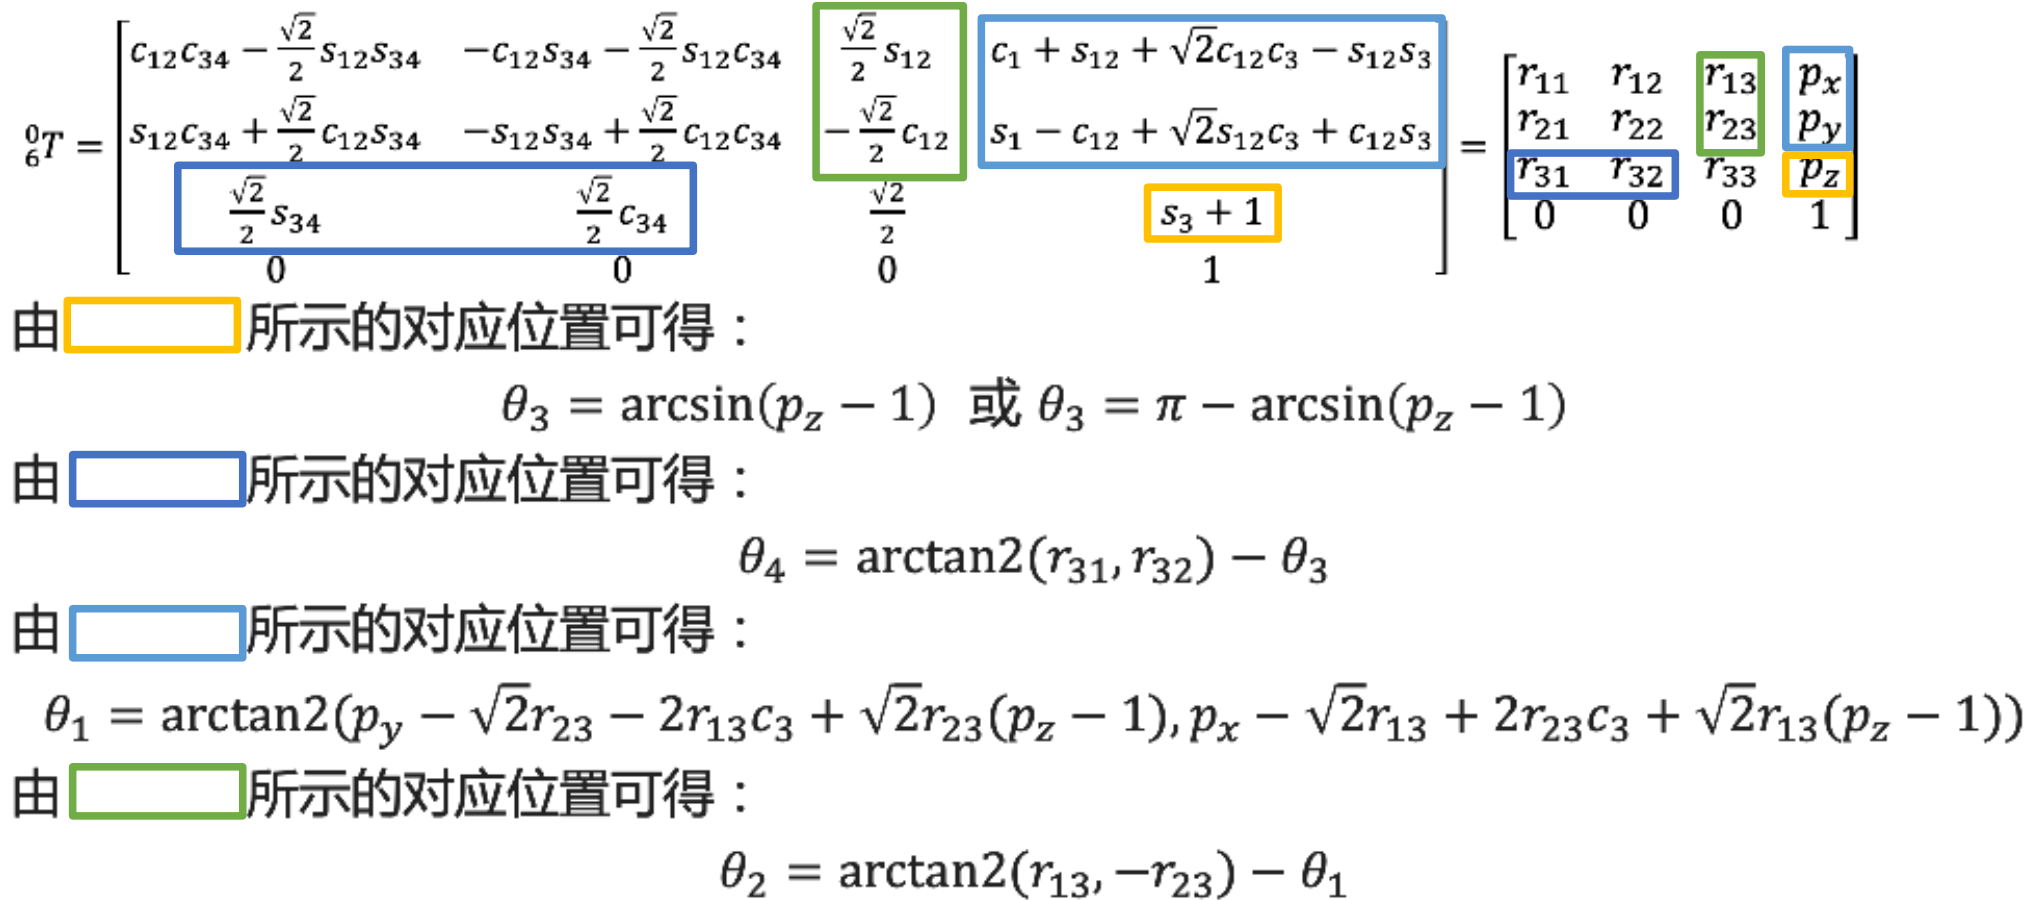
\includegraphics[width=0.6\textwidth]{2.2} 
\caption{逆运动学例题2}
\end{figure}
%------------------------------------------------
\subsubsection[解的讨论]{解的讨论}
\begin{itemize}
\item 存在:目标点是否超出工作空间,代数上为反三角函数定义域,几何上为三角不等式。
\item 多解:由反三角函数多解(尽量使用$ atan2(y, x) $保证解唯一)引起,需关注不同解对应的空间构型。
\item 奇异:自由度丢失,表现为除零。
\end{itemize} 
%------------------------------------------------
\subsection[工作空间]{工作空间}
%------------------------------------------------
\paragraph{概念}
\begin{itemize}
\item 工作空间(W):末端能到达的空间。
\item 可达空间(RW):机器人至少能以一种姿态到达的空间。
\item 灵巧空间(DW):末端能以任意姿态到达的空间。
\item $ DW \subset RW = W $。
\end{itemize} 
%------------------------------------------------
\paragraph{灵巧空间}\tip{灵巧空间}
腕部工作空间以末端执行器长为半径内外切圆。 \\
\noindent
\begin{minipage}{0.6\textwidth}
\begin{figure}[H]
\centering
\subfloat[圆环状]{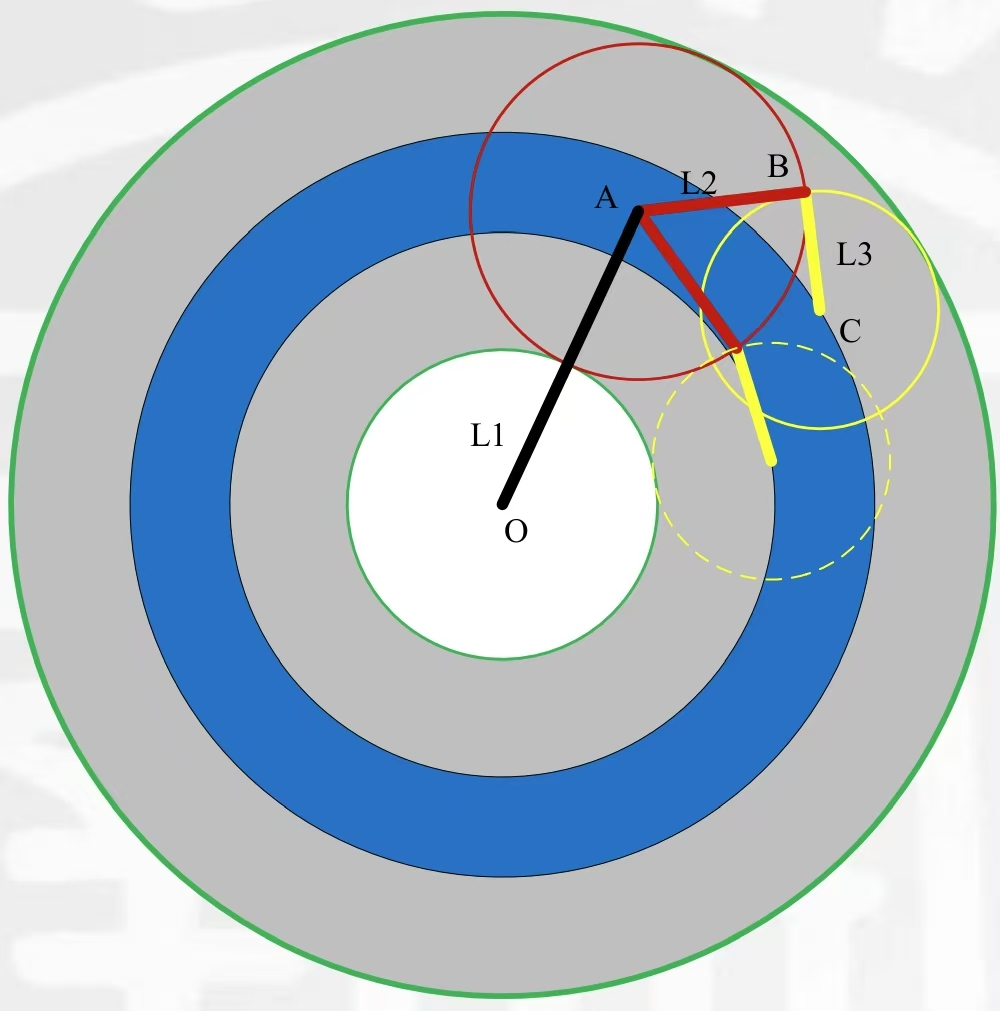
\includegraphics[width=.3\textwidth]{space1}} \quad
\subfloat[内圆外环]{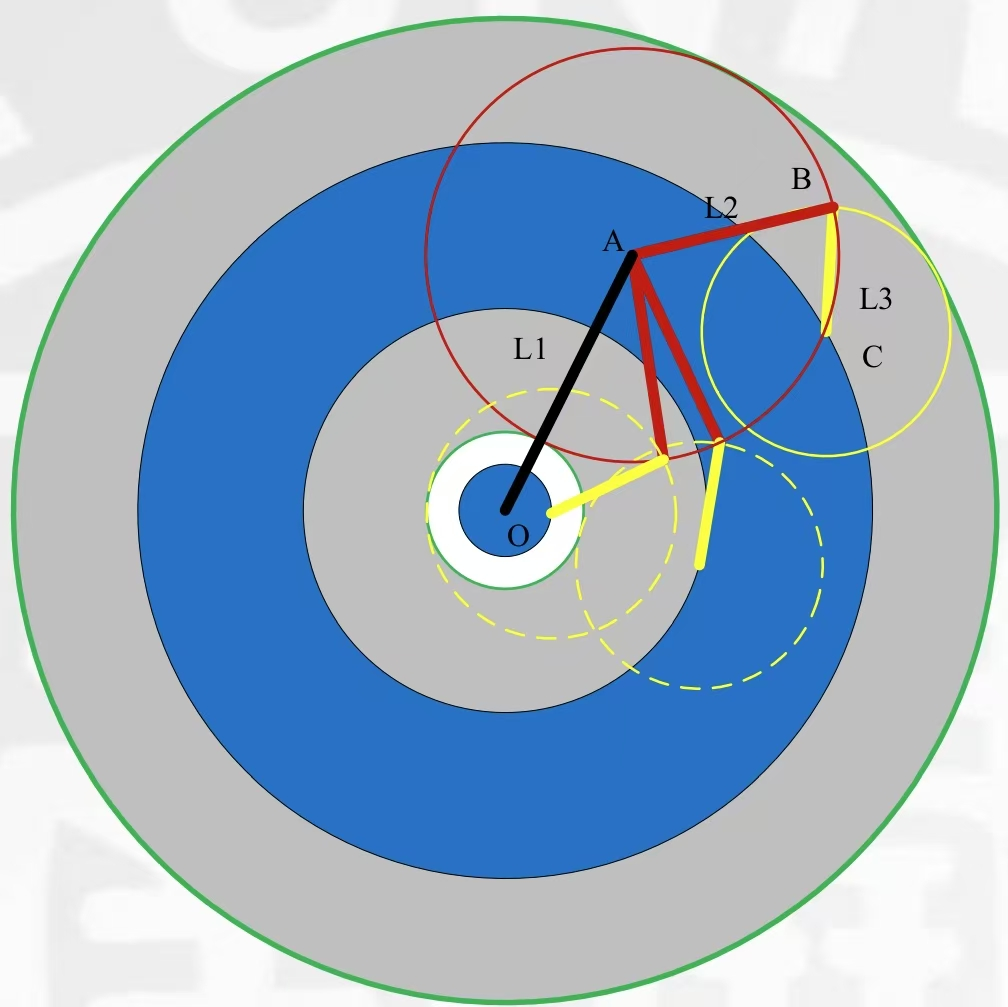
\includegraphics[width=.3\textwidth]{space2}} \quad
\subfloat[大圆]{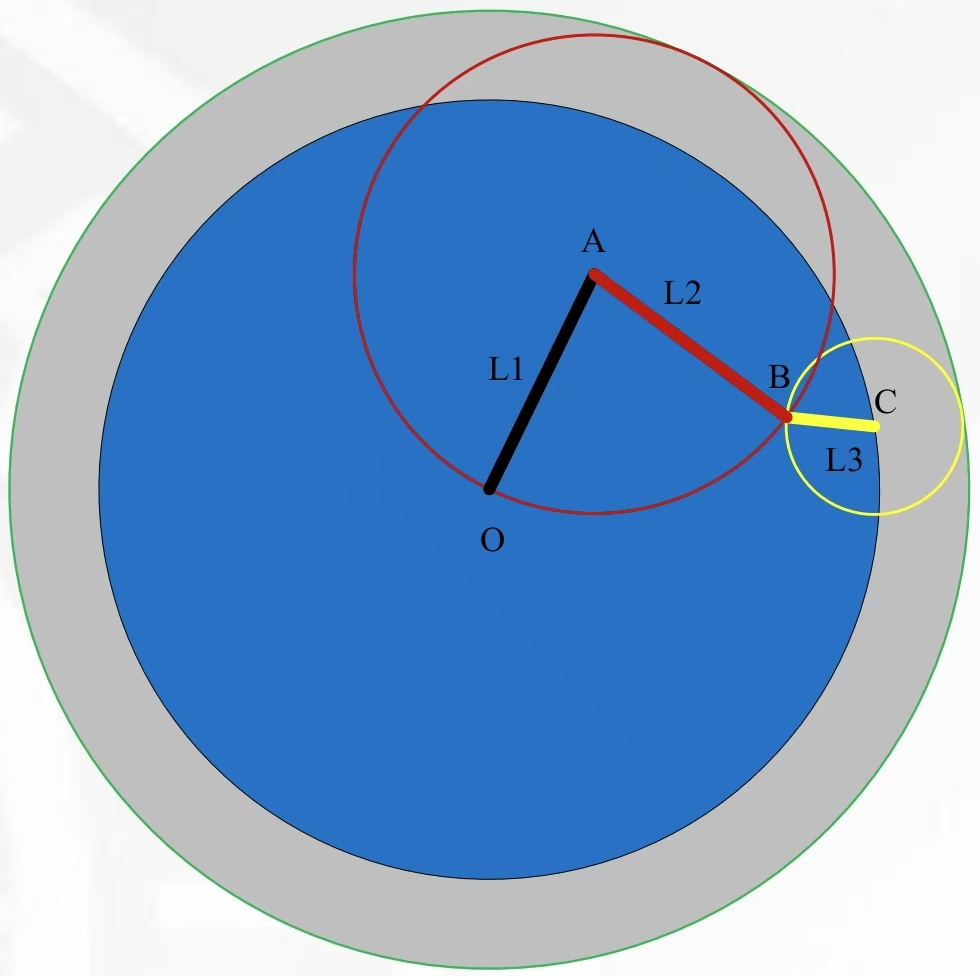
\includegraphics[width=.3\textwidth]{space5}} \\
\subfloat[内圆]{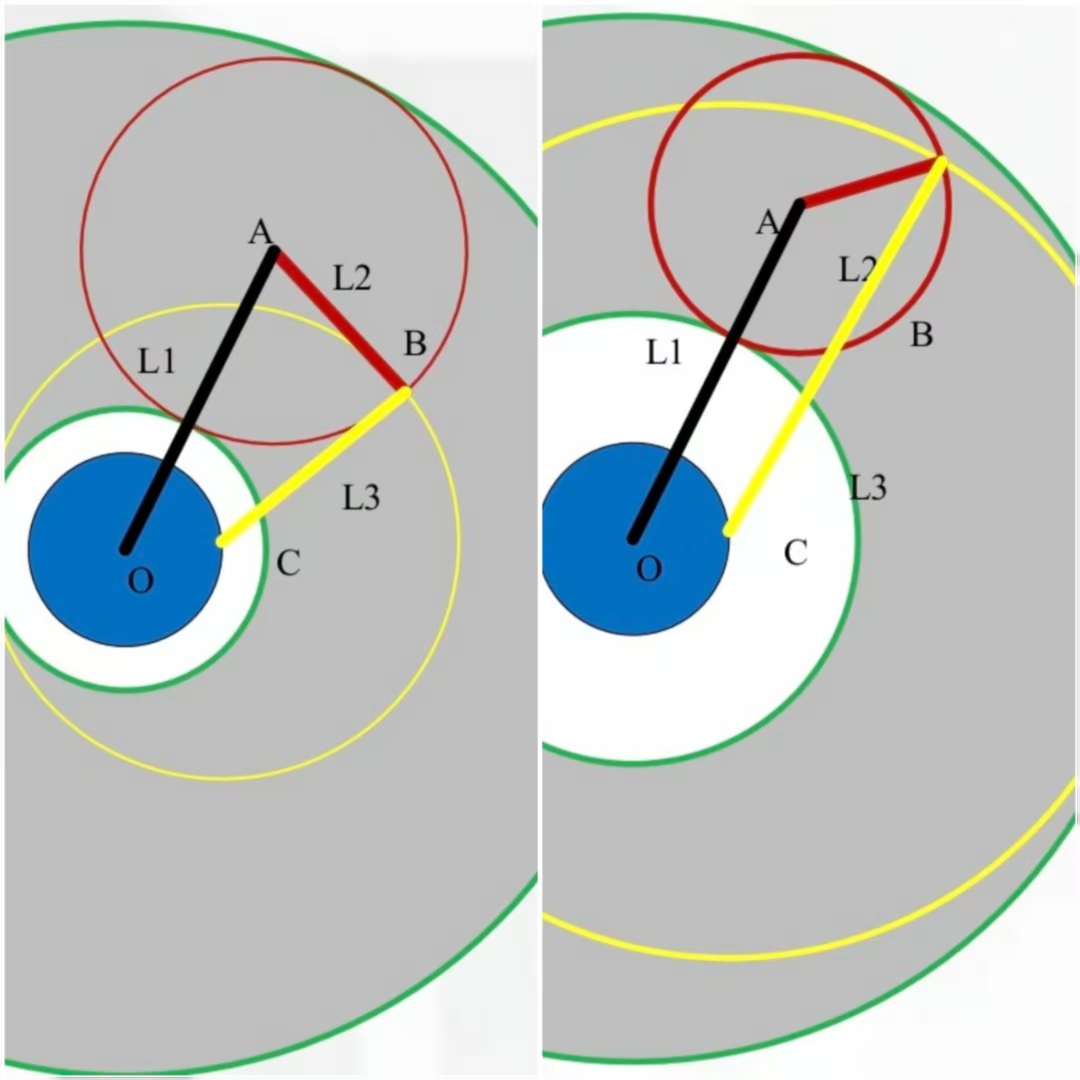
\includegraphics[width=.3\textwidth]{space3}} \quad
\subfloat[无]{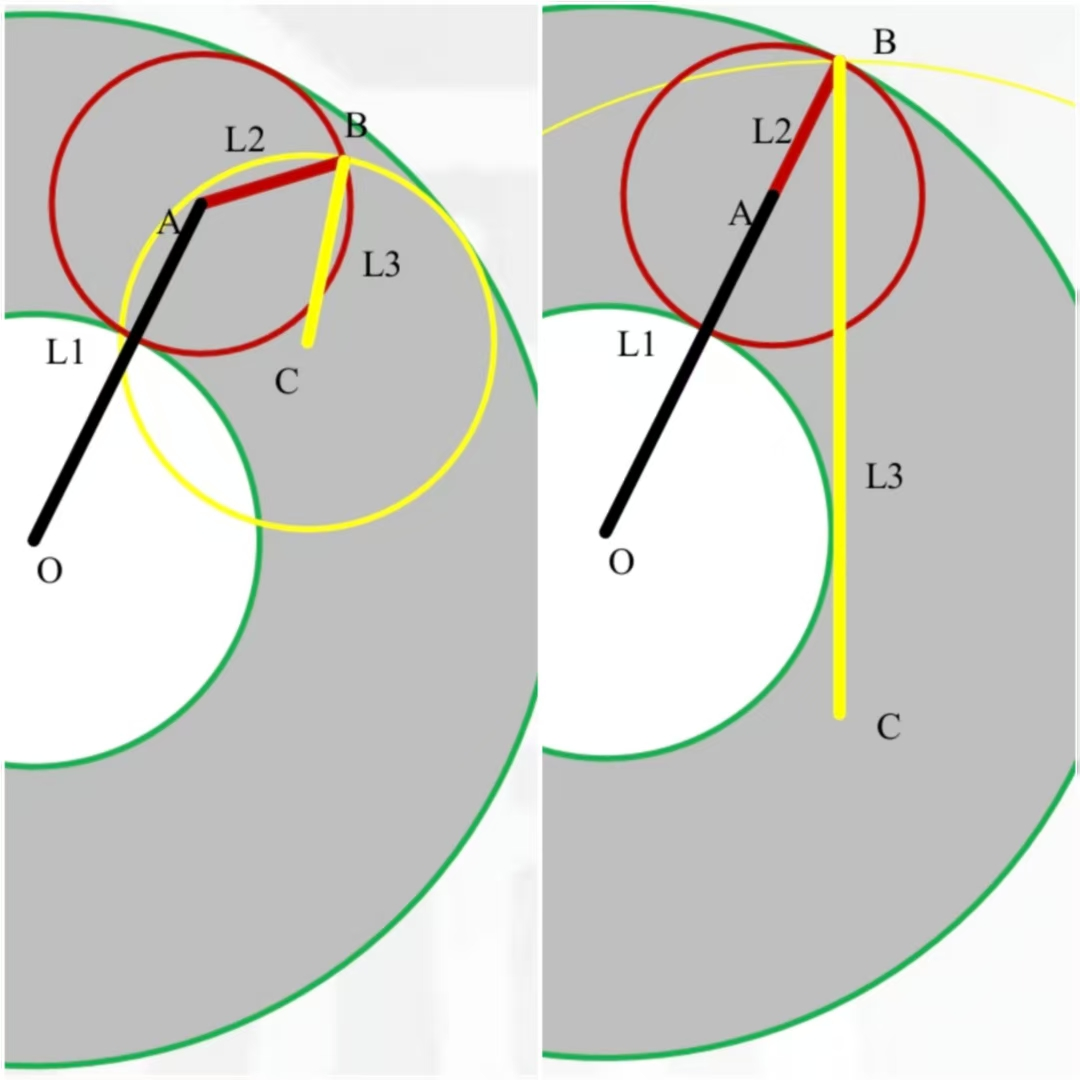
\includegraphics[width=.3\textwidth]{space4}}
\caption{3R操作臂灵巧空间}
\end{figure}
\end{minipage}
\begin{minipage}{0.4\textwidth}
{\footnotesize
\hspace{2em}
以下以3R操作臂为例,分析不同臂长情况下的灵巧空间:
\begin{enumerate}
\item $ 2L_3 \leq L_1 + L_2 - |L_1 - L_2|\&L_3 \leq |L_1 - L_2| $。
\item $ 2L_3 \leq L_1 + L_2 - |L_1 - L_2|\&L_3 \geq |L_1 - L_2| $。
\item $ L_3 \leq L_1 + L_2 $。
\item $ 2L_3 \geq L_1 + L_2 - |L_1 - L_2|\&|L_1 - L_2| \leq L_3 \leq L_1 + L_2 $。
\item $ L_2 \leq L_3 \leq |L_1 - L_2|, L_3 \geq L_1 + L_2 $。
\end{enumerate}
}
\end{minipage}

为寻求较大灵巧空间,需要上下臂基本等长,且臂长不过长。
%------------------------------------------------
\paragraph{参数}
\begin{itemize}
\item $ \text{灵巧系数} = \frac{\text{可达角度所占弧长}}{\text{单位圆周长}}_{\text{(平面)}} = \frac{\text{可达角度所占表面积}}{\text{单位球表面积}}_{\text{(空间)}} $。
\item 重复精度:返回示教点精度。
\end{itemize} 
%----------------------------------------------------------------------------------------
\section{雅可比}
%------------------------------------------------
\subsection[雅可比矩阵]{雅可比矩阵}
雅可比矩阵$ J $表示关节状态(平移或旋转,由$ \epsilon $标注)$ q/\theta $($ n $维)变化率与末端位姿$ X $($ m $维)变化率关系,在$ X = f(q) $时有:
\begin{align*}
\delta x_{(m \times 1)} &= \begin{bmatrix} \frac{\partial f_1}{\partial q_1} & \cdots & \frac{\partial f_1}{\partial q_n} \\ \vdots & \ddots & \vdots \\ \frac{\partial f_m}{\partial q_1} & \cdots & \frac{\partial f_m}{\partial q_n} \end{bmatrix}_{(m \times n)} \delta q_{(n \times 1)} \Leftrightarrow \delta X = J(\theta) \delta \theta \\
J_{ij}(q) &= \frac{\partial}{\partial q_j} f_i(q)
\end{align*}
%------------------------------------------------
\subsection[不同坐标描述下的雅可比矩阵转换]{不同坐标描述下的雅可比矩阵转换\tip{不同坐标描述下的雅可比矩阵转换}}
基础雅可比矩阵(笛卡尔坐标系):
$$ \begin{bmatrix} v \\ \omega \end{bmatrix}_{(6 \times 1)} = J_0(q)_{(6 \times n)} \dot{q}_{(n \times 1)} $$

$ X_P, X_R $定义了坐标描述方式,$ E_P, E_R $则描述了对应的转换关系:
\begin{align*}
\dot{X}_P &= E_P \cdot v = [E_P \cdot J_v] \dot{q} = J_P \dot{q} \\
\dot{X}_R &= E_R \cdot \omega = [E_R \cdot J_\omega] \dot{q} = J_R \dot{q}
\end{align*}

有:
$$ J = \begin{bmatrix} J_P \\ J_R \end{bmatrix} = \begin{bmatrix} E_P & 0 \\ 0 & E_R \end{bmatrix} \begin{bmatrix} J_v \\ J_\omega \end{bmatrix} $$
%------------------------------------------------
\paragraph{线雅可比}
\begin{itemize}
\item 柱坐标系
$
\begin{cases}
\rho = \sqrt{x^2 + y^2} \\
\theta = \arctan(y / x) \\
z = z
\end{cases}
\Rightarrow
E_P(X) = \begin{pmatrix} \cos\theta & \sin\theta & 0 \\ \frac{-\sin\theta}{\rho} & \frac{\cos\theta}{\rho} & 0 \\ 0 & 0 & 1 \end{pmatrix}
$。
\item 球坐标系
$
\begin{cases}
\rho = \sqrt{x^2 + y^2 + z^2} \\
\theta = \arctan(\frac{y}{x}) \\
\phi = \arctan(\frac{\sqrt{x^2 + y^2}}{z})
\end{cases}
\Rightarrow
E_P(X) = \begin{pmatrix} \cos\theta \sin\phi & \sin\theta \sin\phi & \cos\phi \\ \frac{-\sin\theta}{\rho \sin\phi} & \frac{\cos\theta}{\rho \sin\phi} & 0 \\ \frac{\cos\theta \cos\phi}{\rho} & \frac{\sin\theta \cos\phi}{\rho} & \frac{-\sin\phi}{\rho} \end{pmatrix}
$。
\end{itemize} 
%------------------------------------------------
\paragraph{角雅可比}
\begin{itemize}
\item 旋转阵推基础\label{sec:Rotation_matrix}

旋转阵导数为$ \dot{R} = \lim_{\Delta t \to 0} [\frac{R_K(\Delta\theta) - I_3}{\Delta t} R(t)] $,

其与逆(转置)的积为反对称阵$ \dot{R} R^{-1} = \dot{R} R^T = \hat{\Omega} = \begin{bmatrix} 0 & -\Omega_z & \Omega_y \\ \Omega_z & 0 & -\Omega_x \\ -\Omega_y & \Omega_x & 0 \end{bmatrix} $

得到
$
\begin{cases}
\Omega_x = \dot{r}_{31} r_{21} + \dot{r}_{32} r_{22} + \dot{r}_{33} r_{23} \\
\Omega_y = \dot{r}_{11} r_{31} + \dot{r}_{12} r_{32} + \dot{r}_{13} r_{33} \\
\Omega_z = \dot{r}_{21} r_{11} + \dot{r}_{22} r_{12} + \dot{r}_{23} r_{13}
\end{cases}
$,

$ \Omega = \begin{bmatrix} \Omega_x & \Omega_y & \Omega_z \end{bmatrix}^T = \begin{bmatrix} k_x & k_y & k_z \end{bmatrix}^T $为瞬时旋转轴。

例题\ref{sec:example4.2}。
\item 基础推旋转角

对于Z-Y-Z欧拉角(X-Y-Z固定角)$ X_R = \begin{bmatrix} \alpha & \beta & \gamma \end{bmatrix}^T $,有:
$$
\begin{bmatrix} \Omega_x \\ \Omega_y \\ \Omega_z \end{bmatrix}
= \underbrace{\begin{bmatrix} 0 & -s\alpha & c\alpha s\beta \\ 0 & c\alpha & s\alpha s\beta \\ 1 & 0 & c\beta \end{bmatrix}}_{\text{按旋转轴依次提取旋转阵对应列}} \begin{bmatrix} \dot{\alpha} \\ \dot{\beta} \\ \dot{\gamma} \end{bmatrix}
\Rightarrow \begin{bmatrix} \dot{\alpha} \\ \dot{\beta} \\ \dot{\gamma} \end{bmatrix}
= \underbrace{\begin{bmatrix} \frac{c\alpha c\beta}{s\beta} & -\frac{s\alpha c\beta}{s\beta} & 1 \\ -\frac{s\alpha}{s\beta} & \frac{c\alpha}{s\beta} & 0 \\ c\alpha & s\alpha & 0 \end{bmatrix}}_{E_R} \begin{bmatrix} \Omega_x \\ \Omega_y \\ \Omega_z \end{bmatrix}
$$
\end{itemize} 
%------------------------------------------------
\subsection[求导法]{求导法}
%------------------------------------------------
\subsubsection[方法]{方法\tip{求导求雅可比}}
\begin{itemize}
\item 直接法:对正运动学方程直接求导。
$$ J = \begin{bmatrix} \frac{\partial X_P}{\partial q_1} & \frac{\partial X_P}{\partial q_2} & \cdots & \frac{\partial X_P}{\partial q_N} \\ \frac{\partial x_R}{\partial q_1} & \frac{\partial x_R}{\partial q_2} & \cdots & \frac{\partial x_R}{\partial q_N} \end{bmatrix} $$
\item 旋转阵法:线雅可比直接求导,角雅可比提取各旋转阵$ Z $列(原理见\ref{sec:Terminal_function})。\label{sec:Terminal_function_back}
\end{itemize} 
$$ J = \begin{bmatrix} \frac{\partial X_P}{\partial q_1} & \frac{\partial X_P}{\partial q_2} & \cdots & \frac{\partial X_P}{\partial q_N} \\ \overline{\epsilon}_1 Z_1 & \overline{\epsilon}_2 Z_2 & \cdots & \overline{\epsilon}_n Z_n \end{bmatrix} $$
%------------------------------------------------
\subsubsection[例题]{例题\tip{求导求雅可比例题}}
%------------------------------------------------
\paragraph{例题1}
{\footnotesize
以下以斯坦福臂(2RP3R)为例:

\begin{figure}[H]
\centering
\subfloat[斯坦福臂结构图]{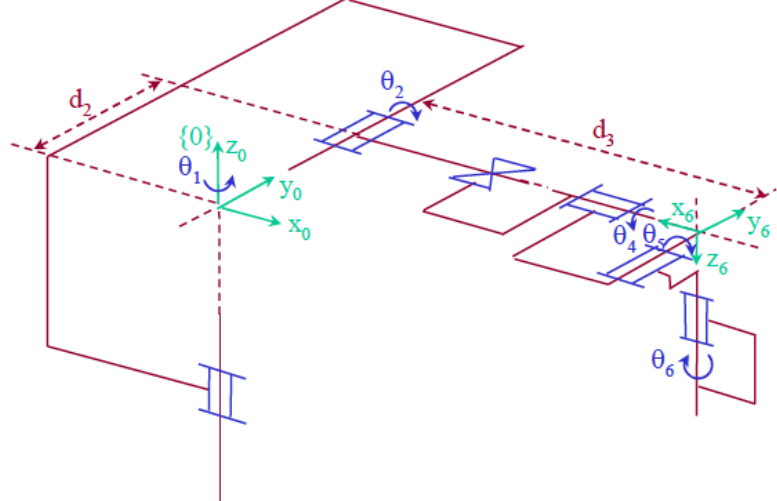
\includegraphics[width=.4\textwidth]{4.1}} \quad
\subfloat[参数表]{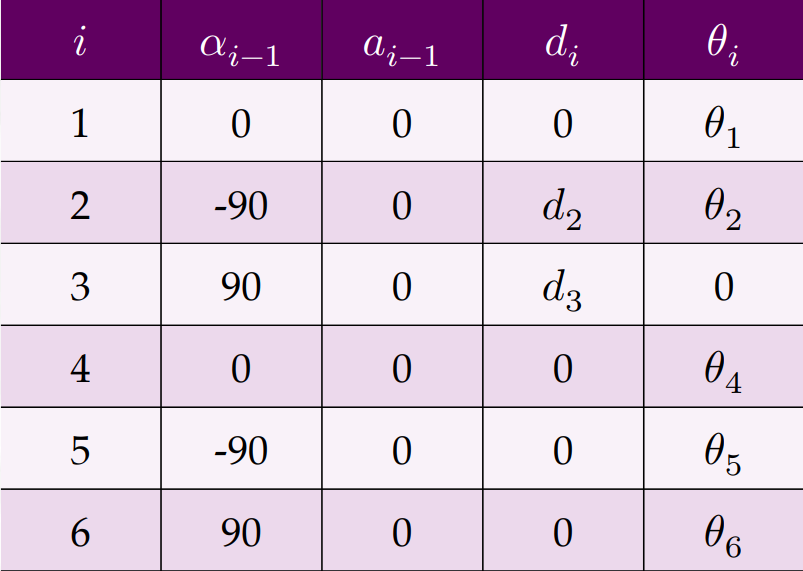
\includegraphics[width=.35\textwidth]{4.2}}
\caption{旋转阵法求雅可比例题1}
\end{figure}

$ {}_6^0 T = {{}_1^0 T}{{}_2^1 T}{{}_3^2 T}{{}_4^3 T}{{}_5^4 T}{{}_6^5 T} $得到正运动学方程,将其提取为列向量:
$$ X = \begin{bmatrix} X_P \\ r_1 \\ r_2 \\ \textcolor{red}{r_3} \end{bmatrix} = \begin{bmatrix} d_3 c1 s2 - d_2 s1 \\ d_3 s1 s2 + d_2 c1 \\ d_3 c2 \\ {r_1}_{(3 \times 1)} \\ {r_2}_{(3 \times 1)} \\ \textcolor{red}{c1(c2 c4 s5 + s2 c5) - s1 s4 s5} \\ \textcolor{red}{s1(c2 c4 s5 + s2 c5) + c1 s4 s5} \\ \textcolor{red}{-s2 c4 s5 + c2 c5} \end{bmatrix} $$

雅可比矩阵为:
\begin{align*}
J &= \begin{bmatrix} Z_1 \times P_{13} & Z_2 \times P_{23} & Z_3 & Z_4 \times 0 & Z_5 \times 0 & Z_6 \times 0 \\ Z_1 & Z_2 & 0 & Z_4 & Z_5 & Z_6 \end{bmatrix}
= \begin{bmatrix} \frac{\partial X_P}{\partial q_1} & \frac{\partial X_P}{\partial q_2} & \frac{\partial X_P}{\partial q_3} & 0 & 0 & 0 \\ Z_1 & Z_2 & 0 & Z_4 & Z_5 & \textcolor{red}{Z_6} \end{bmatrix} \\
&= \begin{bmatrix} -(d_3 s1 s2 + d_2 c1) & c1 c2 d_3 & c1 s2 & 0 & 0 & 0 \\ d_3 c1 s2 - d_2 s1 & s1 c2 d_3 & s1 s2 & 0 & 0 & 0 \\ 0 & -s2 d_3 & c2 & 0 & 0 & 0 \\ 0 & -s1 & 0 & c1 s2 & -c1 c2 s4 - s1 c4 & \textcolor{red}{c1 c2 c4 s5 - s1 s4 s5 + c1 s2 c5} \\ 0 & c1 & 0 & s1 s2 & -s1 c2 s4 + c1 c4 & \textcolor{red}{s1 c2 c4 s5 + c1 s4 s5 + s1 s2 c5} \\ 1 & 0 & 0 & c2 & s2 s4 & \textcolor{red}{-s2 c4 s5 + c2 c5} \end{bmatrix}
\end{align*}

以上省略了中间的齐次变换阵,它们旋转阵$ Z $列对应各$ Z_i $。

在$ \theta_5 = k\pi $时,奇异,简化为(第4列和第6列相同):
$$ \begin{bmatrix} x & x & x & 0 & 0 & 0 \\ x & x & x & 0 & 0 & 0 \\ x & x & x & 0 & 0 & 0 \\ 0 & x & 0 & c1 s2 & x & c1 s2 \\ 0 & x & 0 & s1 s2 & x & s1 s2 \\ x & 0 & 0 & c2 & x & c2 \end{bmatrix} $$
}
%------------------------------------------------
\paragraph{例题2}\label{sec:example4.2}
{\footnotesize
3R机器人正运动学方程为:
$$ {}_3^0 T = \begin{bmatrix} c1 c23 & -c1 s23 & s1 & l_1 c1 + l_2 c1 c2 \\ s1 c23 & -s1 s23 & -c1 & l_1 s1 + l_2 s1 c2 \\ s23 & c23 & 0 & l_2 s2 \\ 0 & 0 & 0 & 1 \end{bmatrix} $$

对平移向量和旋转阵分别求偏导,得到:
$$
{}^0 J_v(\theta) = \begin{bmatrix} -l_1 s1 - l_2 s1 c2 & -l_2 c1 s2 & 0 \\ l_1 c1 + l_2 c1 c2 & -l_2 s1 s2 & 0 \\ 0 & l_2 c2 & 0 \end{bmatrix},
{}^0 J_R(\theta) = \begin{bmatrix} -s1 c23 & -c1 s23 & -c1 s23 \\ s1 s23 & -c1 c23 & -c1 c23 \\ c1 & 0 & 0 \\ c1 c23 & -s1 s23 & -s1 s23 \\ -c1 s23 & -s1 c23 & -s1 c23 \\ s1 & 0 & 0 \\ 0 & c23 & c23 \\ 0 & -s23 & -s23 \\ 0 & 0 & 0 \end{bmatrix}
$$

可转化$ {}^0 J_R(\theta) $为基础角雅可比(见\ref{sec:Rotation_matrix}),结果略。
}
%------------------------------------------------
\subsection[速度传播法]{速度传播法}
%------------------------------------------------
\subsubsection[串行逐连杆求解]{串行逐连杆求解\tip{串行速度传播求雅可比}}
由连杆$ k $起始端速度,求其末端速度,进而获得连杆$ k + 1 $起始端速度。

\begin{figure}[H]
\centering 
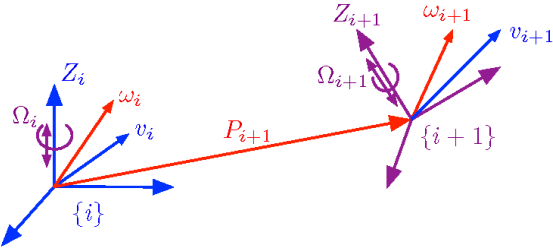
\includegraphics[width=0.4\textwidth]{Velocity propagation} 
\caption{串行速度传播}
\end{figure}

\begin{itemize}
\item 平移关节:线速度传导 + 角速度转换线速度 + 平移变化。
$$
v_{i + 1} = v_i + \omega_i \times P_{i + 1} + \dot{d}_{i + 1} \cdot Z_{i + 1}
\overset{\text{换系}}{\Longrightarrow}
{}^{i + 1}v_{i + 1} = {}^{i + 1}_i R \cdot ({}^i v_i + {}^i \omega_i \times {}^i P_{i + 1}) + \dot{d}_{i + 1} \cdot {}^{i + 1}Z_{i + 1}
$$
\item 旋转关节:角速度传导 + 旋转变化。
$$
\Omega_{i + 1} = \dot{\theta}_{i + 1} \cdot Z_{i + 1}, \omega_{i + 1} = \omega_i + \Omega_{i + 1}
\overset{\text{换系}}{\Longrightarrow}
{}^{i + 1}\omega_{i + 1} = {}^{i + 1}_i R \cdot {}^i \omega_i + \dot{\theta}_{i + 1} \cdot {}^{i + 1}Z_{i + 1}
$$
\end{itemize} 
%------------------------------------------------
\subsubsection[并行末端作用求解]{并行末端作用求解\tip{并行速度传播求雅可比}}
%------------------------------------------------
\paragraph{单关节作用}\label{sec:bingxing}
求一关节运动对末端运动影响时,将其他连杆固定,视为刚体。 \\
\noindent
\begin{minipage}{0.6\textwidth}
\begin{figure}[H]
\centering 
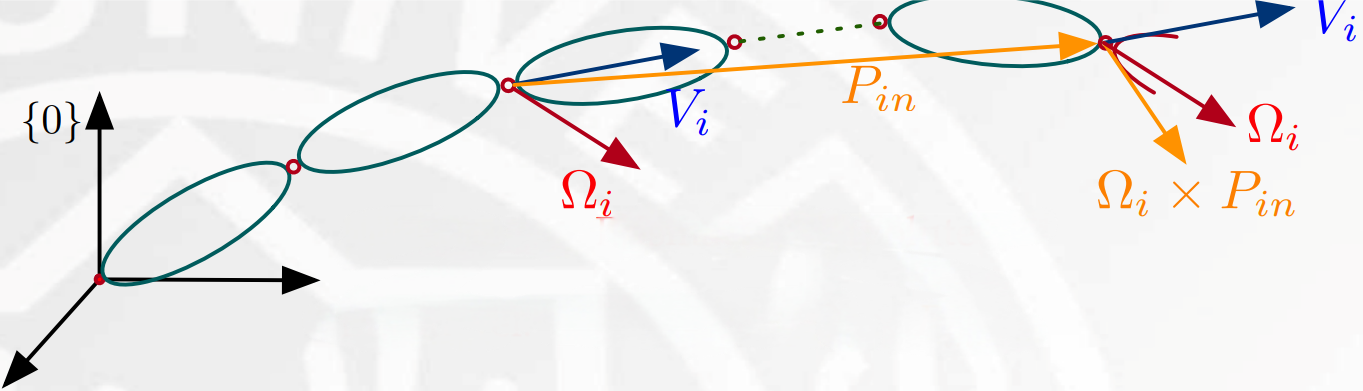
\includegraphics[width=0.8\textwidth]{Terminal function} 
\caption{并行速度传播}
\end{figure}
\end{minipage}
\hfill
\begin{minipage}{0.35\textwidth}
\begin{table}[H]
\centering
\begin{tabular}{c|cc}
\hline
& 平移关节 & 旋转关节 \\
\hline
线速度 & $ V_i $ & $ \Omega_i \times P_{in} $ \\
角速度 & $ 0 $ & $ \Omega_i $ \\
\hline
\end{tabular}
\caption{并行速度传播}
\end{table}
\end{minipage}
\begin{itemize}
\item 线速度 = 线速度传导 + 角速度转换线速度。
\item 角速度 = 角速度传导。
\end{itemize} 

回到雅可比转换\ref{sec:bingxing_back1},回到惯性阵$ M(q) $求取\ref{sec:bingxing_back2}。
%------------------------------------------------
\paragraph{综合作用}\label{sec:Terminal_function}
基于基坐标系,由$ V_i = Z_i \dot{q}_i, \Omega_i = Z_i \dot{q}_i $,综合各关节运动,得到:
\begin{align*}
v &= \sum_{i = 1}^n [\epsilon_i V_i + \overline{\epsilon}_i (\Omega_i \times P_{in})] = \sum_{i = 1}^n [\epsilon_i Z_i + \overline{\epsilon}_i (Z_i \times P_{in})] \dot{q}_i \\
\omega &= \sum_{i = 1}^n \overline{\epsilon}_i \Omega_i = \sum_{i = 1}^n (\overline{\epsilon}_i Z_i) \dot{q}_i
\end{align*}

回到旋转阵法\ref{sec:Terminal_function_back}。
%------------------------------------------------
\subsection[静态力传播法]{静态力传播法\tip{静态力传播求雅可比}}
%------------------------------------------------
\subsubsection[静态力与力矩]{静态力与力矩}\label{sec:fn1}
由末端往回推,根据各连杆力与力矩平衡进行求解。

对于连杆$ i $,$ f_i, n_i $表示自身受力(矩),$ -f_{i + 1}, -n_{i + 1} $表示下一连杆的反作用力(矩),$ P $表示连杆长度,有:
$$
\begin{cases}
f_i = f_{i + 1} \\
n_i = n_{i + 1} + P_{i + 1} \times f_{i + 1}
\end{cases}
\overset{\text{换系}}{\Longrightarrow}
\begin{cases}
{}^i f_i = {}^i_{i + 1}R \cdot {}^{i + 1} f_{i + 1} \\
{}^i n_i = {}^i_{i + 1}R \cdot {}^{i + 1} n_{i + 1} + {}^i P_{i + 1} \times {}^i f_i
\end{cases}
$$
\noindent
\begin{minipage}{0.65\textwidth}
\begin{figure}[H]
\centering
\subfloat[静力学受力分析]{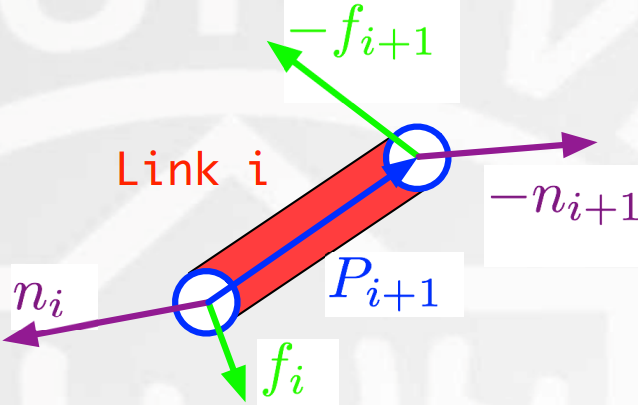
\includegraphics[width=.3\textwidth]{force}} \quad
\subfloat[平移关节]{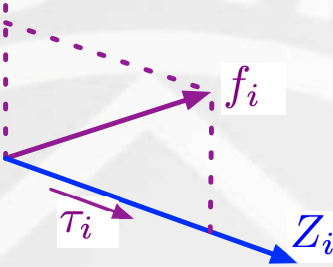
\includegraphics[width=.25\textwidth]{Prismatic Joint}} \quad
\subfloat[旋转关节]{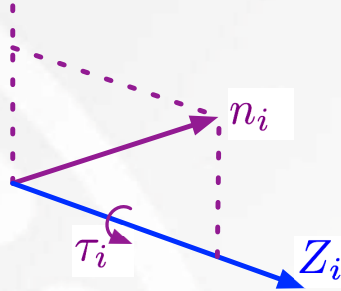
\includegraphics[width=.25\textwidth]{Revolute Joint}}
\caption{静态力与力矩}
\end{figure}
\end{minipage}
\begin{minipage}{0.35\textwidth}
\begin{table}[H]
\centering
\begin{tabular}{c|cc}
\hline
& 平移关节 & 旋转关节 \\
\hline
计算量 & 力 & 力矩 \\
计算 & $ \tau_i = f_i^T Z_i $ & $ \tau_i = n_i^T Z_i $ \\
内部平衡量 & 力矩 & 力 \\
\hline
\end{tabular}
\caption{力与力矩(动静一致)}
\end{table}
\end{minipage}

与动力学受力分析对比\ref{sec:fn2}。
%------------------------------------------------
\subsubsection[速度与扭矩]{速度与扭矩}
\noindent
\begin{minipage}{0.6\textwidth}
\begin{figure}[H]
\centering
\subfloat[角速度与线速度]{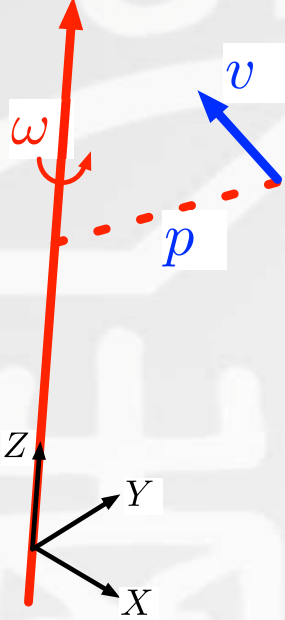
\includegraphics[width=.2\textwidth]{wv}} \quad
\subfloat[力与扭矩]{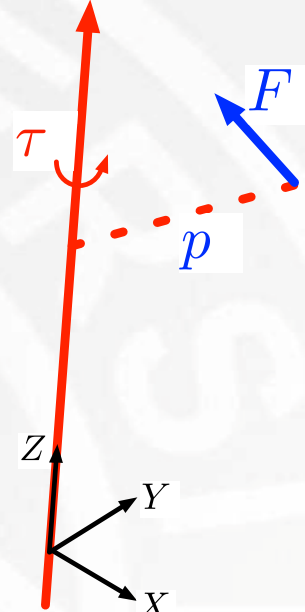
\includegraphics[width=.2\textwidth]{ft}}
\caption{速度与扭矩}
\end{figure}
\end{minipage}
\begin{minipage}{0.4\textwidth}
\begin{align*}
v &= \omega \times p = -\hat{p} \omega = J \dot{\theta} \\
\tau &= p \times F = -\hat{p}^T F = J^T F
\end{align*}
\end{minipage}
%------------------------------------------------
\subsubsection[虚功原理]{虚功(Virtual Work)原理\tip{虚功原理}}
已知各连杆力(矩),微小移动$ \delta x $下,各力(矩)作功之和为$ \delta W = \sum_i f_i \delta x_i $,在其等于$ 0 $时,各力(矩)所作功抵消,即:
$$ \tau^T \delta q + (-F)^T \delta x = 0 \overset{\delta x = J \delta q}{\Longrightarrow} \tau = J^T F $$

其中$ J $是末端雅可比,而非腕部雅可比。
%------------------------------------------------
\subsubsection[例题]{例题\tip{扭矩与虚功原理例题}}
\begin{figure}[H]
\centering 
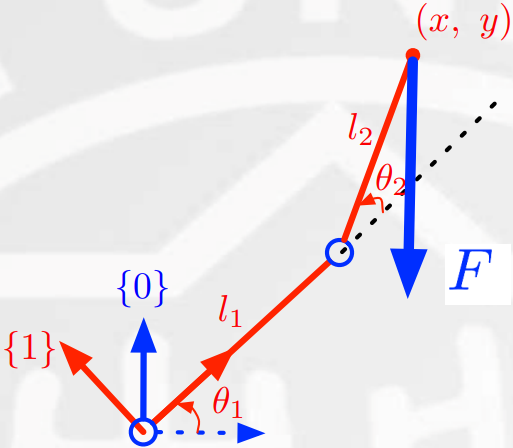
\includegraphics[width=0.25\textwidth]{5} 
\caption{扭矩与虚功原理例题}
\end{figure}

{\footnotesize
条件: $ l_1 = l_2 = 1, \theta_1 = 0, \theta_2 = 60^\circ, F = \begin{bmatrix} 0 & -1 & 0 \end{bmatrix}^T N $。
\begin{enumerate}
\item 求力矩:
\begin{itemize}
\item 对于连杆2:$ f_2 = F, n_2 = \vec{l}_2 \times F = \begin{bmatrix} 0 & 0 & -l_2 \cos(\theta_1 + \theta_2) \end{bmatrix}^T N $。
\item 对于连杆1:$ f_1 = f_2 = F, n_1 = n_2 + \vec{l}_1 \times f_2 = \begin{bmatrix} 0 & 0 & -l_1 \cos\theta_1 - l_2 \cos(\theta_1 + \theta_2) \end{bmatrix}^T N $。
\end{itemize} 
\item 求扭矩:
\begin{itemize}
\item 由几何关系得$ P = \begin{bmatrix} l_1 c1 + l_2 c12 \\ l_1 s1 + l_2 s12 \end{bmatrix} $。
\item 求偏导得$ J = \begin{bmatrix} -(l_1 s1 + l_2 s12) & -l_2 s12 \\ l_1 c1 + l_2 c12 & l_2 c12 \end{bmatrix} $。
\item $ \tau = J^T F = \begin{bmatrix} -(l_1 s1 + l_2 s12) & l_1 c1 + l_2 c12 \\ - l_2 s12 & l_2 c12 \end{bmatrix} \begin{bmatrix} 0 \\ -1 \end{bmatrix} $。
\end{itemize} 
\end{enumerate}
}
%------------------------------------------------
\subsection[雅可比转换]{雅可比转换\tip{雅可比转换}}\label{sec:Jacobian transform}\label{sec:bingxing_back1}
一般求解基坐标系下的腕部雅可比$ ^0 J_j $。
%------------------------------------------------
\paragraph{位置转换}
根据并行求解结论(见\ref{sec:bingxing}),换序+反对称:
$$ \begin{bmatrix} v_j \\ \omega_j \end{bmatrix} = \begin{bmatrix} E & -\hat{P}_{ij} \\ 0 & E \end{bmatrix} \begin{bmatrix} v_i \\ \omega_i \end{bmatrix} \Rightarrow J_j = \begin{bmatrix} E & -\hat{P}_{ij} \\ 0 & E \end{bmatrix} J_i $$ 
%------------------------------------------------
\paragraph{坐标系转换}
$ {}^0 \hat{P}_{ij} = {}^0_n R \cdot {}^n \hat{P}_{ij} \cdot {}^0_n R^T $:
$$ {}^0 J_j = \begin{bmatrix} {}^0_n R & -{}^0_n R \cdot {}^n \hat{P}_{ij} \cdot {}^0_n R^T \\ 0 & {}^0_n R \end{bmatrix} {}^n J_i $$

不同坐标系下$ J $不同,但是$ |J| $相同:$ {}^i J \neq {}^j J, |{}^i J| = |{}^j J| $。
%------------------------------------------------
\subsection[其他]{其他}
%------------------------------------------------
\subsubsection[雅可比奇异]{雅可比奇异\tip{雅可比奇异}}
$ |J(q)| = 0 $时,奇异,存在方向无法运动或旋转,控制失效。
%------------------------------------------------
\subsubsection[雅可比速率控制]{雅可比速率控制}
\begin{figure}[H]
\centering 
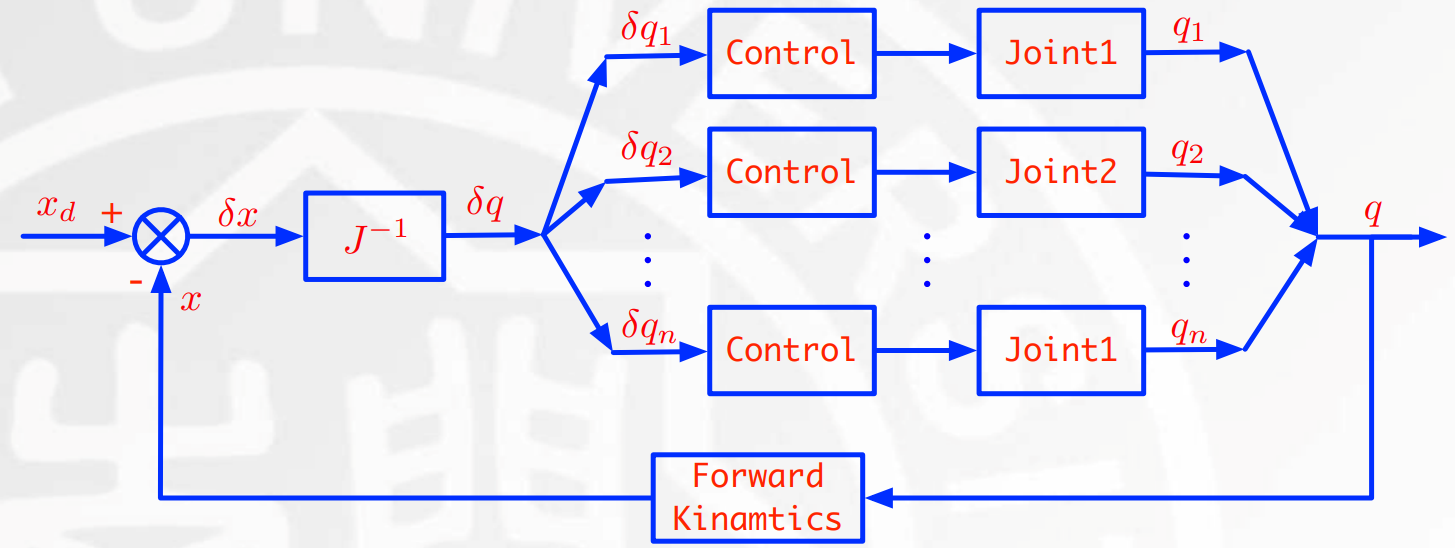
\includegraphics[width=0.6\textwidth]{J_control} 
\caption{雅可比速率控制}
\end{figure}

$ \delta q = J(q)^{-1} \delta x $,为保证可逆,可采用伪逆$ J(q)^+ $。
%------------------------------------------------
\section{动力学}
%------------------------------------------------
\subsection[刚体动力学]{刚体动力学}
%------------------------------------------------
\subsubsection[受力种类分析]{受力种类分析}
\begin{itemize}
\item 惯性参考系
\begin{itemize}
\item 重力$ G $。
\item 惯性力$ F_1 = ma $。
\end{itemize} 
\item 旋转参考系(非惯性参考系):假想力。
\begin{itemize}
\item 离心力$ F_2 = m \omega^2 r $:沿半径背离圆心。
\item 科里奥利力$ F_3 = 2mv' \times \omega $:相对于参考系运动的惯性力(惯性系下保持直线运动)。
\end{itemize} 
\item 合力:$ \Gamma $为广义关节力,$ q,\dot{q},\ddot{q} $为关节空间广义坐标、速度、加速度,$ M(q) $为惯性阵。
\begin{align*}
\Gamma &= ma + m \omega^2 r + 2mv' \times \omega + G \\
&= \textcolor{red}{M(q) \ddot{q} + V(q, \dot{q}) + G(q) (\text{标准形式})}
\end{align*}
\end{itemize} 
%------------------------------------------------
\subsubsection[运动分析]{运动分析\tip{运动分析}}
\begin{figure}[H]
\centering
\subfloat[质点直线运动]{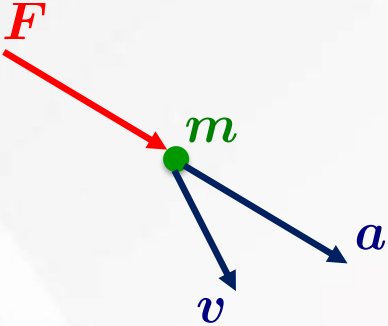
\includegraphics[width=.15\textwidth]{point_p}} \quad
\subfloat[刚体直线运动]{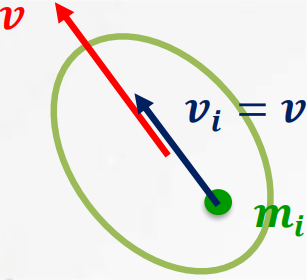
\includegraphics[width=.15\textwidth]{rigid_p}} \quad
\subfloat[质点旋转运动]{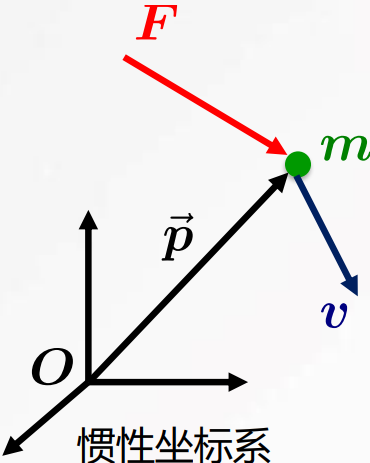
\includegraphics[width=.15\textwidth]{point_r}} \quad
\subfloat[刚体旋转运动]{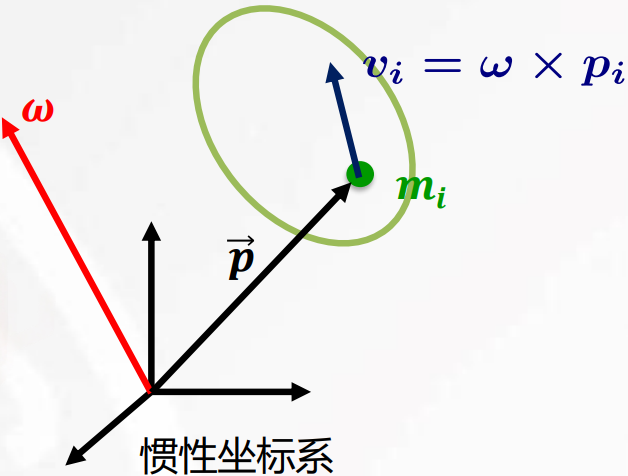
\includegraphics[width=.2\textwidth]{rigid_r}}
\caption{运动分析}
\end{figure}
%------------------------------------------------
\paragraph{直线运动}
\begin{itemize}
\item 动量守恒(合外力为零,系统总动量不变):$ F = ma = m \dot{v} = \dot{Q} $。
\item 动量变化率等于所受外力:
$$ Q = mv \overset{\text{质点到刚体}}{\Longrightarrow} Q = \int_V v_i \rho dV = (\int_V \rho dV) v = mv $$
质量阵$ m = diag(m, m, m) $表明刚体空间运动的各向同性。
\end{itemize} 
%------------------------------------------------
\paragraph{旋转运动}
\begin{itemize}
\item 角动量守恒(合外力为零/指向原点,系统总角动量不变):$ \tau = \vec{p} \times m \dot{v} = \dot{L} $。
\item 角动量变化量等于所受外力矩:
$$ L = \vec{p} \times mv = mp \times (\omega \times p) \overset{\text{质点到刚体}}{\Longrightarrow} L = \int_V p \times (\omega \times p) \rho dV = (\int_V -\hat{p} \hat{p} \rho dV) \omega = I \omega $$
\end{itemize} 
%------------------------------------------------
\subsubsection[惯性张量]{惯性张量$ I $\tip{惯性张量}}
%------------------------------------------------
\paragraph{计算}
$$ -\hat{p} \hat{p} = (p^T p)E_3 - p p^T = \begin{bmatrix} y^2 + z^2 & -xy & -xz \\ -xy & z^2 + x^2 & -yz \\ -xz & -yz & x^2 + y^2 \end{bmatrix} \Rightarrow I = \int_V -\hat{p} \hat{p} \rho dV = \begin{bmatrix} I_{xx} & -I_{xy} & -I_{xz} \\ -I_{xy} & I_{yy} & -I_{yz} \\ -I_{xz} & -I_{yz} & I_{zz} \end{bmatrix} $$

三列分别表示沿$ x, y, z $三轴旋转时,对三轴产生的动量矩列向量$ L = r \times m \omega \times r $。
\begin{itemize}
\item 惯量矩(绕主轴的转动惯量):恒正,和(即$ tr(I) $)不变,绕质心转轴最小。
$$ I_{xx} = \iiint (y^2 + z^2)\rho dxdydz, I_{yy} = \iiint (z^2 + x^2)\rho dxdydz, I_{zz} = \iiint (x^2 + y^2)\rho dxdydz $$
\item 惯量积:可正可负可零。
$$ I_{xy} = \iiint (xy)\rho dxdydz, I_{yz} = \iiint (yz)\rho dxdydz, I_{xz} = \iiint (xz)\rho dxdydz $$
\end{itemize} 
%------------------------------------------------
\paragraph{性质}
\begin{itemize}
\item 平行轴定理:质量为$ m $的刚体,绕通过质心的轴有$ I_C $,移动旋转轴$ p_c $有\\$ I_A = I_C + m[(p_c^T p_c)E_3 - p_c p_c^T] $。
\item 垂直轴定理:对于平面薄板刚体,绕垂直于平面的轴的$ I_Z $为绕与其相交的平面正交轴的$ I_X, I_Y $之和。
\item 两坐标轴分别使刚体质量对称分布,垂直于二者组成的对称平面的第三轴参与的惯性积为$ 0 $。
\item 惯性主轴:两个为零惯性积的公用坐标轴,为物体与转轴的固有属性,与坐标系选取无关。
\item 惯性张量只取决于刚体形状、质量分布和转轴位置,和转动状态(如转速)无关。其特征值为主惯性矩,相应的特征矢量为主轴。
\end{itemize}
%------------------------------------------------
\paragraph{例题}
{\footnotesize
以下以长方体为例,其长宽高分别为$ L, W, H $,密度为$ \rho $: \\
\begin{minipage}{0.25\textwidth}
\begin{figure}[H]
\centering
\subfloat[位于中心]{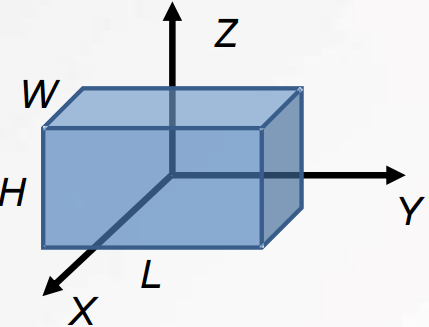
\includegraphics[width=\textwidth]{6.1}} \\
\subfloat[位于一角]{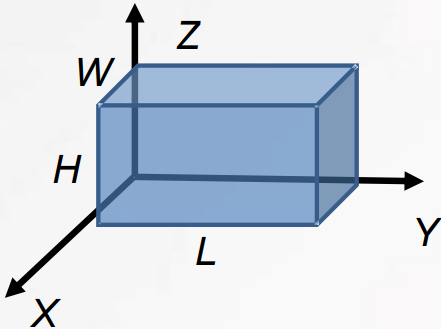
\includegraphics[width=\textwidth]{6.2}}
\caption{惯性张量例题}
\end{figure}
\end{minipage}
\begin{minipage}{0.75\textwidth}
\begin{enumerate}
\item 位于中心:
\begin{align*}
I_{xx} &= \int_{-\frac{H}{2}}^{\frac{H}{2}} \int_{-\frac{L}{2}}^{\frac{L}{2}} \int_{-\frac{W}{2}}^{\frac{W}{2}} (y^2 + z^2)\rho dxdydz = \frac{H^2 + L^2}{12} LWH\rho = \frac{m}{12}(H^2 + L^2) \\
I_{xy} &= \int_{-\frac{H}{2}}^{\frac{H}{2}} \int_{-\frac{L}{2}}^{\frac{L}{2}} \int_{-\frac{W}{2}}^{\frac{W}{2}} (xy)\rho dxdydz = 0
\end{align*}
\item 位于一角,利用平行轴定理:
\begin{align*}
I_{Axx} &= I_{Cxx} + m(y_C^2 + z_C^2) = \frac{m}{12}(H^2 + L^2) + \frac{m}{4}(H^2 + L^2) = \frac{m}{3}(H^2 + L^2) \\
I_{Axy} &= I_{Cxy} + m x_C y_C = \frac{m}{4}WL
\end{align*}
\end{enumerate}
\end{minipage}
}
%------------------------------------------------
\subsection[牛顿-欧拉动力学方程]{牛顿-欧拉动力学方程}
%------------------------------------------------
\subsubsection[推导]{推导}
%------------------------------------------------
\paragraph{动力学受力分析}\label{sec:fn2}
\textcolor{red}{与静力学受力分析对比}\ref{sec:fn1}。 \\
\begin{minipage}{0.3\textwidth}
\begin{figure}[H]
\centering 
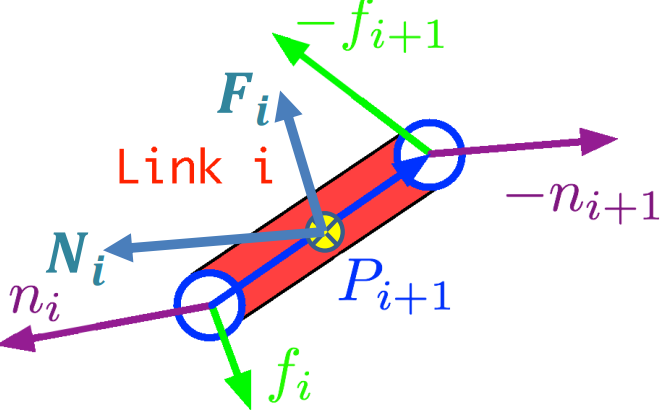
\includegraphics[width=\textwidth]{force2} 
\caption{动力学受力分析}
\end{figure}
\end{minipage}
\begin{minipage}{0.7\textwidth}
$$
\begin{cases}
f_i &= f_{i + 1} \textcolor{red}{+ F_i} \\
n_i &= n_{i + 1} + P_{i + 1} \times f_{i + 1} \textcolor{red}{+ P_{C_i} \times F_i + N_i} \\
\end{cases}
$$
\end{minipage}
%------------------------------------------------
\paragraph{牛顿-欧拉动力学方程}
\begin{itemize}
\item 牛顿方程:$ F = \dot{Q} = ma $。
\item 欧拉方程:$ N = \dot{L} = \frac{d}{dt}(\vec{m}||\omega||) = \dot{\vec{m}}||\omega|| + \vec{m}||\dot{\omega}|| = \omega \times \vec{m}||\omega|| + I \dot{\omega} = \omega \times I \omega + I \dot{\omega} $。
\end{itemize}
%------------------------------------------------
\paragraph{关节分析(外推)}
\begin{figure}[H]
\centering
\subfloat[速度与加速度]{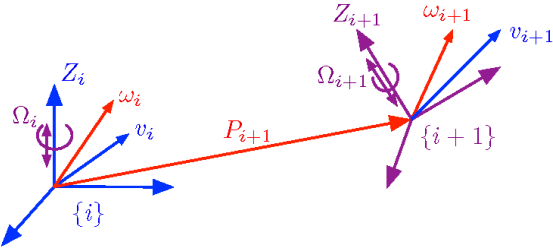
\includegraphics[width=.4\textwidth]{Velocity propagation}} \quad
\subfloat[受力]{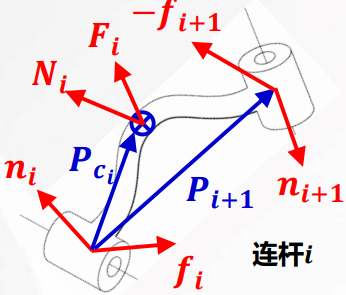
\includegraphics[width=.2\textwidth]{Force Analysis}}
\caption{关节分析}
\end{figure}

\begin{itemize}
\item 速度:
\begin{align*}
v_{i + 1} &=  v_i + \omega_i \times P_{i + 1} + \dot{d}_{i + 1} \cdot Z_{i + 1} \\
\omega_{i + 1} &=  \omega_i + \dot{\theta}_{i + 1} \cdot Z_{i + 1}
\end{align*}
\item 加速度:(\textcolor{blue}{平移关节})
\begin{align*}
\dot{v}_{i + 1} &=  \dot{v}_i +  \dot{\omega}_i \times P_{i + 1} + \textcolor{blue}{\ddot{d}_{i + 1} \cdot Z_{i + 1}} + \underbrace{\omega_i \times \overset{\omega_i \times P_{i + 1}}{\overbrace{\dot{P_{i + 1}}}}}_{\text{离心力}} + \underbrace{\textcolor{blue}{2\dot{d}_{i + 1} \omega_i \times Z_{i + 1}}}_{\text{科里奥利力}} \\
\dot{\omega}_{i + 1} &=  \dot{\omega}_i + \ddot{\theta}_{i + 1} \cdot Z_{i + 1} + \dot{\theta}_{i + 1} \cdot \underbrace{\dot{Z_{i + 1}}}_{\omega_i \times Z_{i + 1}}
\end{align*}
\item 质心处速度:($ P_{C_{i + 1}} $为起始到质心的向量)
\begin{align*}
v_{C_{i + 1}} &= v_{i + 1} + \omega_{i + 1} \times P_{C_{i + 1}} \\
\omega_{C_{i + 1}} &= \omega_{i + 1}
\end{align*}
\item 质心处速度:
\begin{align*}
\dot{v}_{C_{i + 1}} &= \dot{v}_{i + 1} + \dot{\omega}_{i + 1} \times P_{C_{i + 1}} + \omega_{i + 1} \times (\omega_{i + 1} \times P_{C_{i + 1}}) \\
\dot{\omega}_{C_{i + 1}} &= \dot{\omega}_{i + 1}
\end{align*}
\item 连杆惯性力(矩):
\begin{align*}
F_{i + 1} &= m_{i + 1} \dot{v}_{C_{i + 1}} \\
N_{i + 1} &= I_{C_{i + 1}} \dot{\omega}_{i + 1} + \omega_{i + 1} \times I_{C_{i + 1}} \omega_{i + 1}
\end{align*}
\item 质心处受力分析:
\begin{align*}
F_i &= f_i - f_{i + 1} = m_i \dot{v}_{C_i} \\
N_i &= n_i - n_{i + 1} + (-P_{C_i}) \times f_i + (P_{i + 1} - P_{C_i}) \times (-f_{i + 1})
\end{align*}
\end{itemize}
%------------------------------------------------
\subsubsection[总结]{总结}
%------------------------------------------------
\noindent
\begin{minipage}{0.6\textwidth}
\paragraph{步骤}\tip{牛顿-欧拉动力学方程}
\begin{enumerate}
\item 初始化(基坐标系固定时表征重力):
$$ {}^0 \omega_0 = 0, {}^0 v_0 = 0, {}^0 \dot{v}_0 = g $$
\item 外推:
\begin{enumerate}
\item 关节速度、加速度。
\item 质心速度、加速度。
\item 质心处受力(矩)。
\end{enumerate}
\item 内推:关节力(矩)。
\item 标准形式:$ \Gamma = M(q) \ddot{q} + V(q, \dot{q}) + G(q) $。
\end{enumerate}
\end{minipage}
\begin{minipage}{0.4\textwidth}
\begin{figure}[H]
\centering 
\includegraphics[width=\textwidth]{Newton Euler} 
\caption{牛顿-欧拉建模过程}
\end{figure}
\end{minipage}
%------------------------------------------------
\paragraph{统一坐标系:}
\begin{align*}
{}^{i + 1}v_{i + 1} &= \textcolor{red}{{}^{i + 1}_i R} \cdot {}^i v_i + \textcolor{red}{{}^{i + 1}_i R}(\textcolor{blue}{{}^i \omega_i} \times \textcolor{cyan}{{}^i P_{i + 1}}) + \textcolor{violet}{\dot{d}_{i + 1}} \cdot \textcolor{magenta}{{}^{i + 1}Z_{i + 1}} \\
\textcolor{orange}{{}^{i + 1}\omega_{i + 1}} &= \textcolor{red}{{}^{i + 1}_i R} \cdot \textcolor{blue}{{}^i \omega_i} + \textcolor{teal}{\dot{\theta}_{i + 1}} \cdot \textcolor{magenta}{{}^{i + 1}Z_{i + 1}} \\
\textcolor{pink}{{}^{i + 1}\dot{v}_{i + 1}} &= \textcolor{red}{{}^{i + 1}_i R} \cdot [{}^i \dot{v}_i + {}^i \dot{\omega}_i \times \textcolor{cyan}{{}^i P_{i + 1}} + \textcolor{blue}{{}^i \omega_i} \times (\textcolor{blue}{{}^i \omega_i} \times \textcolor{cyan}{{}^i P_{i + 1}})] + \ddot{d}_{i + 1} \cdot \textcolor{magenta}{{}^{i + 1} Z_{i + 1}} + 2\textcolor{violet}{\dot{d}_{i + 1}} \cdot {}^{i + 1}\omega_i \times \textcolor{magenta}{{}^{i + 1}Z_{i + 1}} \\
\textcolor{purple}{{}^{i + 1}\dot{\omega}_{i + 1}} &= \textcolor{red}{{}^{i + 1}_i R} \cdot {}^i \dot{\omega}_i + \ddot{\theta}_{i + 1} \cdot \textcolor{magenta}{{}^{i + 1}Z_{i + 1}} + \textcolor{teal}{dot{\theta}_{i + 1}} \cdot (\textcolor{red}{{}^{i + 1}_i R} \cdot \textcolor{blue}{{}^i \omega_i} \times \textcolor{magenta}{{}^{i + 1}Z_{i + 1}}) \\
\textcolor{brown}{{}^{i + 1}\dot{v}_{C_{i + 1}}} &= \textcolor{pink}{{}^{i + 1}\dot{v}_{i + 1}} + \textcolor{purple}{{}^{i + 1}\dot{\omega}_{i + 1}} \times \textcolor{lime}{{}^{i + 1}P_{C_{i + 1}}} + \textcolor{orange}{{}^{i + 1}\omega_{i + 1}} \times (\textcolor{orange}{{}^{i + 1}\omega_{i + 1}} \times \textcolor{lime}{{}^{i + 1}P_{C_{i + 1}}}) \\
{}^{i + 1}F_{i + 1} &= m_{i + 1} \cdot \textcolor{brown}{{}^{i + 1}\dot{v}_{C_{i + 1}}} \\
{}^{i + 1}N_{i + 1} &= \textcolor{yellow}{{}^{i + 1}I_{C_{i + 1}}} \cdot \textcolor{purple}{{}^{i + 1}\dot{\omega}_{i + 1}} + \textcolor{orange}{{}^{i + 1}\omega_{i + 1}} \times \textcolor{yellow}{{}^{i + 1}I_{C_{i + 1}}} \cdot \textcolor{orange}{{}^{i + 1}\omega_{i + 1}} \\
\textcolor{gray}{{}^i f_i} &= {}^i F_i + \textcolor{green}{{}^i_{i + 1}R} \cdot {}^{i + 1}f_{i + 1} \\
\textcolor{olive}{{}^i n_i} &= {}^i N_i + \textcolor{green}{{}^i_{i + 1}R} \cdot {}^{i + 1}n_{i + 1} + {}^i P_{C_i} \times {}^i F_i + \textcolor{cyan}{{}^i P_{i + 1}} \times \textcolor{green}{{}^i_{i + 1}R} \cdot {}^{i + 1}f_{i + 1} \\
\tau_i &= 
\begin{cases} 
\textcolor{olive}{{}^i n_i} \cdot Z_i & \text{旋转关节} \\ 
\textcolor{gray}{{}^i f_i} \cdot Z_i & \text{平移关节} 
\end{cases}
\end{align*}
%------------------------------------------------
\subsection[拉格朗日动力学算法]{拉格朗日动力学算法}
%------------------------------------------------
\subsubsection[拉格朗日动力学方程]{拉格朗日动力学方程}
%------------------------------------------------
\paragraph{系统能量分析}
\begin{itemize}
\item 势能$ U(q, t) $:
\begin{itemize}
\item 与速度:无关,$ \textcolor{red}{\frac{\partial U}{\partial \dot{q}} = 0} $。
\item 与位移:克服的弹力或重力,$ \textcolor{green}{\frac{\partial U}{\partial q} = G(q)} $。
\end{itemize}
\item 动能$ K(q, \dot{q}, t) = \frac{1}{2}\dot{q}^T M(q) \dot{q} $(其中$ q $为$ v/\omega $,$ M $为$ M/I $):瞬时性,正标量。
\begin{itemize}
\item 与速度:(角)动量,$ \textcolor{orange}{\frac{\partial K}{\partial \dot{q}} = Q(q, \dot{q})} $,其变化率为惯性力$ \textcolor{orange}{F = \frac{d Q(q, \dot{q})}{d t}} $。
\item 与位移(构型变化):内力做功,$ \textcolor{blue}{\frac{\partial K}{\partial q} = \frac{\partial M(q)}{\partial q}} $。
\end{itemize}
\end{itemize}
%------------------------------------------------
\paragraph{拉格朗日动力学方程}
系统输入(广义外力)$ \Gamma $与相互独立的广义坐标和广义速度$ q,\dot{q} \in R^n $的关系:
\begin{align*}
\Gamma &= \underbrace{\textcolor{orange}{\frac{d}{d t}\frac{\partial K}{\partial \dot{q}}} - \textcolor{blue}{\frac{\partial K}{\partial q}}}_{\text{非惯性系力}M(q) \ddot{q} + V(q, \dot{q})} + \underbrace{\textcolor{green}{\frac{\partial U}{\partial q}}}_{\text{重力}G(q)} \\
&= \frac{d}{d t}\frac{\partial(K - \textcolor{red}{U})}{\partial \dot{q}} - \frac{\partial(K - U)}{\partial q} \\
&= \frac{d}{d t}\frac{\partial L}{\partial \dot{q}} - \frac{\partial L}{\partial q}
\end{align*}

对于各关节有:
$$ \tau_i = \frac{d}{d t}\frac{\partial L(q, \dot{q}, t)}{\partial \dot{q}_i} - \frac{\partial L(q, \dot{q}, t)}{\partial q_i} \quad i = 1, 2, \cdots, N $$
%------------------------------------------------
\subsubsection[求解]{求解}
%------------------------------------------------
\paragraph{动能}
\begin{align*}
\frac{\partial}{\partial\dot{q}}K(q, \dot{q}) &= M(q) \dot{q} \Rightarrow \frac{d}{d t}(\frac{\partial}{\partial \dot{q}}K(q, \dot{q})) = M(q) \ddot{q} + \dot{M}(q) \dot{q} \\
\frac{\partial}{\partial q}K(q, \dot{q}) &= \frac{\partial}{\partial q}[\frac{1}{2}\dot{q}^T M(q) \dot{q}] = \frac{1}{2} \begin{bmatrix} \dot{q}^T \frac{\partial M(q)}{\partial q_1}\dot{q} \\ \vdots \\ \dot{q}^T \frac{\partial M(q)}{\partial q_N}\dot{q} \end{bmatrix}
\end{align*}

所以:
$$ \frac{d}{dt}\frac{\partial K(q, \dot{q})}{\partial\dot{q}} - \frac{\partial K(q, \dot{q})}{\partial q} = \underbrace{M(q) \ddot{q}}_{\text{惯性力}} + \underbrace{\dot{M}(q) \dot{q} - \frac{1}{2}\begin{bmatrix} \dot{q}^T \frac{\partial M(q)}{\partial q_1}\dot{q} \\ \vdots \\ \dot{q}^T \frac{\partial M(q)}{\partial q_N}\dot{q} \end{bmatrix}}_{\text{科里奥利力}} $$
%------------------------------------------------
\paragraph{$ M(q) $}\label{sec:bingxing_back2}~\\

连杆$ i $动能$ K_i(q, \dot{q}) = \frac{1}{2}v_{C_i}^T mv_{C_i} + \frac{1}{2}\omega_{C_i}^T I_C \omega_{C_i} $,故机器人系统总动能:
\begin{align*}
K(q, \dot{q}) = \frac{1}{2}\dot{q}^T \textcolor{red}{M(q)} \dot{q} &\equiv \sum_{i = 1}^{n}(\frac{1}{2}v_{C_i}^T m_i v_{C_i} + \frac{1}{2}\omega_{C_i}^T I_{C_i} \omega_{C_i}) \\
&= \sum_{i = 1}^{n}(\frac{1}{2}\dot{q}^T J_{v_{C_i}}^T m_i J_{v_{C_i}} \dot{q} + \frac{1}{2}\dot{q}^T J_{\omega_{C_i}}^T I_{C_i} J_{\omega_{C_i}} \dot{q}) \\
&= \frac{1}{2}\dot{q}^T \textcolor{red}{\sum_{i = 1}^{n}[J_{v_{C_i}}^T m_i J_{v_{C_i}} + J_{\omega_{C_i}}^T I_{C_i} J_{\omega_{C_i}}]} \dot{q}
\end{align*}

其中$ J_{v_{C_i}}, J_{\omega_{C_i}} $为连杆$ i $质心处的线、角雅可比。
\begin{itemize}
\item $ J_{v_{C_i}} $可由$ J_{v_i} $转化(见\ref{sec:bingxing})推得,也可由质心处的位置矢量求偏导获得。
$$ J_{v_{C_i}} = \begin{bmatrix} \frac{\partial P_{C_i}}{\partial q_1} & \frac{\partial P_{C_i}}{\partial q_2} & \cdots & \frac{\partial P_{C_i}}{\partial q_i} & 0 & 0 & \cdots & 0 \end{bmatrix} $$
\item $ J_{\omega_{C_i}} = J_{\omega_i} = \begin{bmatrix} \bar{\epsilon}_1 Z_1 & \bar{\epsilon}_2 Z_2 & \cdots & \bar{\epsilon}_i Z_i & 0 & 0 & \cdots & 0 \end{bmatrix} $,其中,平移关节值为$ 0 $,未涉及到的变化(即关节$ i $之后的变化)值为$ 0 $。
\end{itemize}
$$ M(q) = \begin{bmatrix} m_{11} & m_{12} & \cdots & m_{1n} \\ m_{21} & m_{22} & \cdots & m_{2n} \\ \vdots & \vdots & \ddots & \vdots \\ m_{n1} & m_{n2} & \cdots & m_{nn} \end{bmatrix}_{n \times n} $$
\begin{itemize}
\item $ M(q) $为正定对称阵。
\item $ m_{ii}(q_{i + 1}, \dots, q_n) $描述了机器人在$ q_{i + 1} $到$ q_i $的状态决定构型下的惯量,其只与$ i $关节后的变量有关,故$ m_{nn} $是个定值。
\item 理解:由最后一个关节开始组装,每向回增加一个关节,添加一行一列,表征当前关节与其他关节的耦合作用。
\end{itemize}
%------------------------------------------------
\paragraph{$ V(q, \dot{q}) $}
\begin{itemize}
\item 记号:$ b_{i,j,k} = b_{j,i,k} = \frac{\partial m_{ij}}{\partial q_k}, c_{i,j k} = b_{i,j,k} + b_{i,k,j}, c_{ijk} = \frac{1}{2}(b_{i,j,k} + b_{i,k,j} - b_{j,k,i}) $。
\item 总体:
$$ V(q, \dot{q}) = \textcolor{red}{\dot{M}(q) \dot{q}} - \frac{1}{2}\textcolor{blue}{\begin{bmatrix} \dot{q}^T \frac{\partial M(q)}{\partial q_1}\dot{q} \\ \vdots \\ \dot{q}^T \frac{\partial M(q)}{\partial q_n}\dot{q} \end{bmatrix}} $$
\item 前者:
$$ \dot{M}(q) = \frac{\partial M(q)}{\partial q}\dot{q} = \begin{bmatrix} m'_{11} & m'_{12} & \cdots & m'_{1n} \\ m'_{21} & m'_{22} & \cdots & m'_{2n} \\ \vdots & \vdots & \ddots & \vdots \\ m'_{n1} & m'_{n2} & \cdots & m'_{nn} \end{bmatrix} $$

其中$ m'_{ij} = \sum_{x = 1}^n \frac{\partial m_{ij}}{\partial q_x}\dot{q}_x $。乘以速度矢量$ \dot{q} $得到:
$$ \textcolor{red}{\dot{M}(q) \dot{q}} = \begin{bmatrix} p_1 & p_2 & \cdots & p_n \end{bmatrix}^T $$

其中$ p_i = \sum_{x = 1}^n \sum_{y = 1}^n \frac{\partial m_{ix}}{\partial q_y}\dot{q}_x \dot{q}_y $,$ x = y $的项对应离心力,$ x \neq y $的项对应科里奥利力。可转化为:
$$
\textcolor{red}{\dot{M}(q) \dot{q}} = \begin{bmatrix} b_{1,1,1} & b_{1,2,2} & \cdots & b_{1,n,n} \\ b_{2,1,1} & b_{2,2,2} & \cdots & b_{2,n,n} \\ \vdots & \vdots & \ddots & \vdots \\ b_{n,1,1} & b_{n,2,2} & \cdots & b_{n,n,n} \end{bmatrix}
\begin{bmatrix} \dot{q}_1^2 \\ \dot{q}_2^2 \\ \vdots \\ \dot{q}_n^2 \end{bmatrix}
+ \begin{bmatrix} c_{1,1 2} & c_{1,1 3} & \cdots & c_{1,n - 1 n} \\ c_{2,1 2} & c_{2,1 3} & \cdots & c_{2,n - 1 n} \\ \vdots & \vdots & \ddots & \vdots \\ c_{n,1 2} & c_{n,1 3} & \cdots & c_{n,n - 1 n} \end{bmatrix}_{n \times \frac{n^2 - n}{2}}
\begin{bmatrix} \dot{q}_1 \dot{q}_2 \\ \dot{q}_1 \dot{q}_3 \\ \vdots \\ \dot{q}_{n - 1} \dot{q}_n \end{bmatrix}_{\frac{n^2 - n}{2}}
$$
\item 后者:
$$ 
\dot{q}^T \frac{\partial M(q)}{\partial q_i}\dot{q} = \sum_{x = 1}^n \sum_{y = 1}^n \frac{\partial m_{xy}}{\partial q_i}\dot{q}_x \dot{q}_y 
= \begin{bmatrix} b_{1,1,i} \\ b_{2,2,i} \\ \cdots \\ b_{n,n,i} \end{bmatrix}^T 
\begin{bmatrix} \dot{q}_1^2 \\ \dot{q}_2^2 \\ \vdots \\ \dot{q}_n^2 \end{bmatrix}
+ \begin{bmatrix} 2b_{1,2,i} \\ 2b_{1,3,i} \\ \cdots \\ 2b_{n - 1,n,i} \end{bmatrix}^T
\begin{bmatrix} \dot{q}_1 \dot{q}_2 \\ \dot{q}_1 \dot{q}_3 \\ \vdots \\ \dot{q}_{n - 1} \dot{q}_n \end{bmatrix}_{\frac{n^2 - n}{2}}
$$

故:
{\footnotesize
$$
\textcolor{blue}{\begin{bmatrix} \dot{q}^T \frac{\partial M(q)}{\partial q_1}\dot{q} \\ \vdots \\ \dot{q}^T \frac{\partial M(q)}{\partial q_n}\dot{q} \end{bmatrix}} 
= \begin{bmatrix} b_{1,1,1} & b_{2,2,1} & \cdots & b_{n,n,1} \\ b_{1,1,2} & b_{2,2,2} & \cdots & b_{n,n,2} \\ \vdots & \vdots & \ddots & \vdots \\ b_{1,1,n} & b_{2,2,n} & \cdots & b_{n,n,n} \end{bmatrix}
\begin{bmatrix} \dot{q}_1^2 \\ \dot{q}_2^2 \\ \vdots \\ \dot{q}_n^2 \end{bmatrix}
+ 2\begin{bmatrix} b_{1,2,1} & b_{1,3,1} & \cdots & b_{n - 1,n,1} \\ b_{1,2,2} & b_{1,3,2} & \cdots & b_{n - 1,n,2} \\ \vdots & \vdots & \ddots & \vdots \\ b_{1,2,n} & b_{1,3,n} & \cdots & b_{n - 1,n,n} \end{bmatrix}_{n \times \frac{n^2 - n}{2}}
\begin{bmatrix} \dot{q}_1 \dot{q}_2 \\ \dot{q}_1 \dot{q}_3 \\ \vdots \\ \dot{q}_{n - 1} \dot{q}_n \end{bmatrix}_{\frac{n^2 - n}{2}}
$$
}
\item 整合:
$$
V(q, \dot{q}) = 
\underbrace{\begin{bmatrix} c_{111} & c_{122} & \cdots & c_{1nn} \\ c_{211} & c_{222} & \cdots & c_{2nn} \\ \vdots & \vdots & \ddots & \vdots \\ c_{n11} & c_{n22} & \cdots & c_{nnn} \end{bmatrix} \begin{bmatrix} \dot{q}_1^2 \\ \dot{q}_2^2 \\ \vdots \\ \dot{q}_n^2 \end{bmatrix}}_{\text{离心力}c(q) \dot{q}^2}
+ \underbrace{2\begin{bmatrix} c_{112} & c_{113} & \cdots & c_{1(n - 1)n} \\ c_{212} & c_{213} & \cdots & c_{1(n - 1)n} \\ \vdots & \vdots & \ddots & \vdots \\ c_{n12} & c_{n13} & \cdots & c_{n(n - 1)n} \end{bmatrix} \begin{bmatrix} \dot{q}_1 \dot{q}_2 \\ \dot{q}_1 \dot{q}_3 \\ \vdots \\ \dot{q}_{n - 1} \dot{q}_n \end{bmatrix}}_{\text{科里奥利力}B(q) \dot{q} \dot{q}}
$$
\end{itemize}
%------------------------------------------------
\paragraph{$ G(q) $}~\\

求解连杆$ i $势能时,将其质心位置矢量投影到重力方向。对各连杆势能求和,得到:
$$ G(q) = -\sum_{i = 1}^{n} m_i J_{v_{C_i}}^T g $$
%------------------------------------------------
\subsubsection[总结]{总结}
%------------------------------------------------
\paragraph{步骤}\tip{拉格朗日动力学方程}
\begin{enumerate}
\item 求解各连杆质心位置矢量$ P_{C_i} $。
\item 求解各连杆质心处雅可比$ J_{v_{C_i}}, J_{\omega_{C_i}} $,前者求偏导,后者取$ z $列。
\item 求解惯性阵$ M(q) $,需检查$ m_{ii} $是否只与$ q_j, j > i $相关。
$$ M(q) = \sum_{i = 1}^{n}[J_{v_{C_i}}^T m_i J_{v_{C_i}} + J_{\omega_{C_i}}^T I_{C_i} J_{\omega_{C_i}}] $$
\item 求解惯性力$ V(q, \dot{q}) $:
\begin{enumerate}
\item $ b_{i,j,k} = \frac{\partial m_{ij}}{\partial q_k} $。
\item $ c_{ijk} = \frac{1}{2}(b_{i,j,k} + b_{i,k,j} - b_{j,k,i}) $。
\item 
$
V(q, \dot{q}) = 
\begin{bmatrix} c_{111} & c_{122} & \cdots & c_{1nn} \\ c_{211} & c_{222} & \cdots & c_{2nn} \\ \vdots & \vdots & \ddots & \vdots \\ c_{n11} & c_{n22} & \cdots & c_{nnn} \end{bmatrix} \begin{bmatrix} \dot{q}_1^2 \\ \dot{q}_2^2 \\ \vdots \\ \dot{q}_n^2 \end{bmatrix}
+ 2\begin{bmatrix} c_{112} & c_{113} & \cdots & c_{1(n - 1)n} \\ c_{212} & c_{213} & \cdots & c_{1(n - 1)n} \\ \vdots & \vdots & \ddots & \vdots \\ c_{n12} & c_{n13} & \cdots & c_{n(n - 1)n} \end{bmatrix} \begin{bmatrix} \dot{q}_1 \dot{q}_2 \\ \dot{q}_1 \dot{q}_3 \\ \vdots \\ \dot{q}_{n - 1} \dot{q}_n \end{bmatrix}
$。
\end{enumerate}
\item 求解重力$ G(q) $:$ G(q) = -\sum_{i = 1}^{n} m_i J_{v_{C_i}}^T g $。
\item 标准形式:$ \Gamma = M(q) \ddot{q} + V(q, \dot{q}) + G(q) $。
\end{enumerate}
%------------------------------------------------
\subsubsection[例题]{例题\tip{动力学例题}}
{\footnotesize
%------------------------------------------------
\paragraph{例题1}~\\
\begin{minipage}{0.3\textwidth}
\begin{figure}[H]
\centering 
\includegraphics[width=0.8\textwidth]{7.1} 
\caption{动力学例题1}
\end{figure}
\end{minipage}
\begin{minipage}{0.7\textwidth}
\hspace{2em}
RP平面机器人的连杆质量分别为$ m_1, m_2 $,连杆质心距关节$ 1 $距离分别为$ l_1, d_2 $,连杆质心处惯性张量分别为:
$$ {{}^{C_1}}I_1 = \begin{bmatrix} I_{xx1} & 0 & 0 \\ 0 & I_{yy1} & 0 \\ 0 & 0 & I_{zz1} \end{bmatrix}, {{}^{C_2}}I_2 = \begin{bmatrix} I_{xx2} & 0 & 0 \\ 0 & I_{yy2} & 0 \\ 0 & 0 & I_{zz2} \end{bmatrix} $$
\hspace{2em}
统一到$ 1 $坐标系下:$ y_1 $与$ z_2 $重合:
$$ {}^1 P_2 = \begin{bmatrix} 0 & q_2 & 0 \end{bmatrix}^T, {}^1 P_{C_2} = \begin{bmatrix} 0 & d_2 & 0 \end{bmatrix}^T $$
\end{minipage}
%------------------------------------------------
\paragraph{牛顿-欧拉动力学方程法}
\begin{enumerate}
\item 初始条件: $ {}^0 \omega_0 = 0, {}^0 v_0 = 0, {}^0 \dot{\omega}_0 = 0, {}^0 \dot{v}_0 = \begin{bmatrix} 0 & g & 0 \end{bmatrix}^T, f_3 = 0, n_3 = 0 $。
\item 关节$ 1 $运动学:
\begin{align*}
{}^1 \omega_1 &= \dot{q}_1 \cdot {}^1 Z_1 = \begin{bmatrix} 0 & 0 & \dot{q}_1 \end{bmatrix}^T \\
{}^1 \dot{\omega}_1 &= \ddot{q}_1 \cdot {}^1 Z_1 = \begin{bmatrix} 0 & 0 & \ddot{q}_1 \end{bmatrix}^T \\
{}^1 \dot{v}_1 &= {}^1_0 R_z(\theta_1) \cdot {}^0 \dot{v}_0 = \begin{bmatrix} gs1 & gc1 & 0 \end{bmatrix}^T \\
{}^1 \dot{v}_{C_1} &= {}^1 \dot{v}_1 + {}^1 \dot{\omega}_1 \times {}^1 P_{C_1} + {}^1 \omega_1 \times ({}^1 \omega_1 \times {}^1 P_{C_1}) = \begin{bmatrix} -l_1 \dot{q}_1^2 + gs1 & -l_1 \ddot{q}_1 + gc1 & 0 \end{bmatrix}^T
\end{align*}
\item 关节$ 1 $力:
\begin{align*}
{}^1 F_1 &= m_1 \cdot {}^1 \dot{v}_{C_1} \\
{}^1 N_1 &= {}^{C_1}I_1 \times {}^1 \dot{\omega}_1 + {}^1 \omega_1 \times {}^{C_1}I_1 \cdot {}^1 \omega_1 = \begin{bmatrix} 0 & 0 & \ddot{q}_1 I_{zz1} \end{bmatrix}^T
\end{align*}
\item 关节$ 2 $运动学:
\begin{align*}
{}^1 \omega_2 &= {}^1 \omega_1 = \begin{bmatrix} 0 & 0 & \dot{q}_1 \end{bmatrix}^T \\
{}^1 \dot{\omega}_2 &= {}^1 \dot{\omega}_1 = \begin{bmatrix} 0 & 0 & \ddot{q}_1 \end{bmatrix}^T \\
{}^1 \dot{v}_2 &= {}^1 \dot{v}_1 + {}^1 \dot{\omega}_1 \times {}^1 P_2 + {}^1 \omega_1 \times ({}^1 \omega_1 \times {}^1 P_2) + \ddot{q}_2 \cdot {}^1 Z_2 + 2\dot{q}_2 \cdot {}^1 \omega_1 \times {}^1 Z_2 \\
&= \begin{bmatrix} -\ddot{q}_1 q_2 - 2\dot{q}_1 \dot{q}_2 + gs1 & -\dot{q}_1^2 q_2 + {\ddot{q}_2}^2 + gc1 & 0 \end{bmatrix}^T \\
{}^1 \dot{v}_{C_2} &= {}^1 \dot{v}_2 + {}^1 \dot{\omega}_2 \times {}^1 P_{C_2} + {}^1 \omega_2 \times ({}^1 \omega_2 \times {}^1 P_{C_2}) \\
&= \begin{bmatrix} -2\dot{q}_1 \dot{q}_2 + gs1 - \ddot{q}_1(d_2 + q_2) & \ddot{q}_2 + gc1 - \dot{q}_1^2(d_2 + q_2) & 0 \end{bmatrix}^T
\end{align*}
\item 关节$ 2 $力:
\begin{align*}
{}^1 F_2 &= m_2 \cdot {}^1 \dot{v}_{C_2} = \begin{bmatrix} -2m_2 \dot{q}_1 \dot{q}_2 + m_2 gs1 - m_2 \dot{q}_1^2 (d_2 + q_2) & m_2 \ddot{q}_2 + m_2 gc1 - m_2 \dot{q}_1^2 (d_2 + q_2) & 0 \end{bmatrix}^T \\
{}^1 N_2 &= {}^{C_2}I_2 \times {}^1 \dot{\omega}_2 + {}^1 \omega_2 \times {}^{C_2}I_2 \cdot {}^1 \omega_2 = \begin{bmatrix} 0 & 0 & \ddot{q}_1 I_{zz2} \end{bmatrix}^T
\end{align*}
\item 关节$ 2 $力矩:
\begin{align*}
{}^1 f_2 &= {}^1 F_2 \\
{}^1 n_2 &= {}^1 N_2 + {}^1 P_{C_2} \times {}^1 F_2 = \begin{bmatrix} 0 & 0 & \ddot{q}_1 I_{zz2} + 2m_2 d_2 \dot{q}_1 \dot{q}_2 - m_2 d_2 gs1 + m_2 d_2 \ddot{q}_1 (d_2 + q_2) \end{bmatrix}^T
\end{align*}
\item 关节$ 1 $力矩:
\begin{align*}
{}^1 f_1 &= {}^1 F_1 + {}^1 f_2 \\
{}^1 n_1 &= {}^1 N_1 + {}^1 n_2 + {}^1 P_{C_1} \times {}^1 F_1 + {}^1 P_2 \times {}^1 f_2 \\
&= \begin{bmatrix} \star & \star & \ddot{q}_1[I_{zz2} + I_{zz1} + m_1 l_1^2 + m_2(d_2 + q_2)^2] + 2m_2 \dot{q}_1 \dot{q}_2(d_2 + q_2) - [m_1 l_1 + m_2(d_2 + q_2)]gs1 \end{bmatrix}^T
\end{align*}
\item 力矩:
\begin{align*}
\tau_2 &= {}^1 f_2 \cdot {}^1 Z_2 = m_2 \ddot{q}_2 + m_2 gc1 - m_2 \dot{q}_1^2 (d_2 + q_2) \\
\tau_1 &= {}^1 n_1 \cdot {}^1 Z_1 = \ddot{q}_1[I_{zz2} + I_{zz1} + m_1 l_1^2 + m_2(d_2 + q_2)^2] + 2m_2 \dot{q}_1 \dot{q}_2(d_2 + q_2) - [m_1 l_1 + m_2(d_2 + q_2)]gs1
\end{align*}
\end{enumerate}
%------------------------------------------------
\paragraph{拉格朗日动力学法}
\begin{enumerate}
\item 质心位置矢量:
$$ {}^0 P_{C_1} = \begin{bmatrix} -l_1 s1 & l_1 c1 & 0 \end{bmatrix}^T, {}^0 P_{C_2} = \begin{bmatrix} -(q_2 + d_2)s1 & (q_2 + d_2)c1 & 0 \end{bmatrix}^T $$
\item 质心处雅可比:
\begin{align*}
{}^0 J_{v_{C_1}} &= \frac{\partial P_{C_1}}{\partial q} = \begin{bmatrix} -l_1 c1 & 0 \\ -l_1 s1 & 0 \\ 0 & 0 \end{bmatrix} & {}^0 J_{v_{C_2}} &= \frac{\partial P_{C_2}}{\partial q} = \begin{bmatrix} -(q_2 + d_2)c1 & -s1 \\ -(q_2 + d_2)s1 & c1 \\ 0 & 0 \end{bmatrix} \\
{}^0 J_{\omega_{C_1}} &= \begin{bmatrix} \bar{\varepsilon}_1 Z_1 & 0 \end{bmatrix} = \begin{bmatrix} 0 & 0 \\ 0 & 0 \\ 1 & 0 \end{bmatrix} & {}^0 J_{\omega_{C_2}} &= \begin{bmatrix} \bar{\varepsilon}_1 Z_1 & \bar{\varepsilon}_2 Z_2 \end{bmatrix} = \begin{bmatrix} 0 & 0 \\ 0 & 0 \\ 1 & 0 \end{bmatrix}
\end{align*}
\item 惯性阵:
\begin{align*}
M(q) &= \sum_{i = 1}^{2} J_{v_{C_i}}^T m_i J_{v_{C_i}} + J_{\omega_{C_i}}^T I_{C_i} J_{\omega_{C_i}} \\
&= \begin{bmatrix} m_1 l_1^2 & 0 \\ 0 & 0 \end{bmatrix} + \begin{bmatrix} I_{zz1} & 0 \\ 0 & 0 \end{bmatrix} + \begin{bmatrix} m_2(d_2 + q_2)^2 & 0 \\ 0 & m_2 \end{bmatrix} + \begin{bmatrix} I_{zz2} & 0 \\ 0 & 0 \end{bmatrix} \\
&= \begin{bmatrix} I_{zz1} + I_{zz2} + m_1 l_1^2 + m_2(d_2 + q_2)^2 & 0 \\ 0 & m_2 \end{bmatrix}
\end{align*}
\item 惯性力:
\begin{align*}
&b_{1,1,1} = b_{1,2,1} = b_{1,2,2} = b_{2,1,1} = b_{2,1,2} = b_{2,2,1} = b_{2,2,2} = 0, b_{1,1,2} = 2m_2(q_2 + d_2) \\
&c_{111} = c_{122} = c_{212} = c_{222} = 0, c_{211} = -m_2(q_2 + d_2), c_{112} = m_2(q_2 + d_2) \\
&V(q, \dot{q}) = \begin{bmatrix} c_{111} & c_{122} \\ c_{211} & c_{222} \end{bmatrix} \begin{bmatrix} \dot{q}_1^2 \\ \dot{q}_2^2 \end{bmatrix} + 2\begin{bmatrix} c_{112} \\ c_{212} \end{bmatrix} \dot{q}_1 \dot{q}_2 = \begin{bmatrix} 0 & 0 \\ -m_2(q_2 + d_2) & 0 \end{bmatrix} \begin{bmatrix} \dot{q}_1^2 \\ \dot{q}_2^2 \end{bmatrix} + \begin{bmatrix} 2m_2(q_2 + d_2) \\ 0 \end{bmatrix} \dot{q}_1 \dot{q}_2
\end{align*}
\item 重力:
\begin{align*}
G(q) &= -(m_1 J_{v_{C_1}}^T g + m_2 J_{v_{C_2}}^T g) \\
&= -\begin{bmatrix} -l_1 c1 & -l_1 s1 & 0 \\ 0 & 0 & 0 \end{bmatrix} \begin{bmatrix} 0 \\ -m_1 g \\ 0 \end{bmatrix} - \begin{bmatrix} -(q_2 + d_2)c1 & -(q_2 + d_2)s1 & 0 \\ -s1 & c1 & 0 \end{bmatrix} \begin{bmatrix} 0 \\ -m_2 g \\ 0 \end{bmatrix} \\
&= \begin{bmatrix} -(m_1 l_1 + m_2(d_2 + q_2))gs1 \\ m_2 gc1 \end{bmatrix}
\end{align*}
\end{enumerate}
%------------------------------------------------
\paragraph{标准形式}
\begin{align*}
\Gamma = \begin{bmatrix} \tau_1 \\ \tau_2 \end{bmatrix} 
&= \begin{bmatrix} \ddot{q}_1[I_{zz2} + I_{zz1} + m_1l_1^2 + m_2(d_2 + q_2)^2] & 0 \\ 0 & m_2 \end{bmatrix} \ddot{q} \\
&+ \begin{bmatrix} 0 & 0 \\ -m_2(d_2 + q_2) & 0 \end{bmatrix} \begin{bmatrix} \dot{q}_1^2\\ \dot{q}_2^2 \end{bmatrix} 
+ \begin{bmatrix} 2m_2(d_2 + q_2) \\ 0 \end{bmatrix} \dot{q}_1 \dot{q}_2 
+ \begin{bmatrix} -[m_1l_1 + m_2(d_2 + q_2)]s1 \\ m_2 c1 \end{bmatrix} g 
\end{align*}
%------------------------------------------------
\paragraph{例题2}~\\
\begin{minipage}{0.4\textwidth}
\begin{figure}[H]
\centering 
\includegraphics[width=0.6\textwidth]{7.2} 
\caption{动力学例题2}
\end{figure}
\end{minipage}
\hfill
\begin{minipage}{0.6\textwidth}
\hspace{2em}
2R平面机器人的连杆质量分别为$ m_1, m_2 $,杆长分别为$ l_1, l_2 $,连杆质心距相邻关节距离分别为$ l_{C_1}, l_{C_2} $,连杆质心处惯性张量分别为:
$$ {{}^{C_1}}I_1 = \begin{bmatrix} I_{xx1} & 0 & 0 \\ 0 & I_{yy1} & 0 \\ 0 & 0 & I_{zz1} \end{bmatrix}, {{}^{C_2}}I_2 = \begin{bmatrix}  I_{xx2} & 0 & 0 \\ 0 & I_{yy2} & 0 \\ 0 & 0 & I_{zz2} \end{bmatrix} $$
\end{minipage}
%------------------------------------------------
\paragraph{牛顿-欧拉动力学方程法}
\begin{enumerate}
\item 初始条件: $ {}^0 \omega_0 = 0, {}^0 v_0 = 0, {}^0 \dot{\omega}_0 = 0, {}^0 \dot{v}_0 = \begin{bmatrix} 0 & g & 0 \end{bmatrix}^T, f_3 = 0, n_3 = 0 $。
\item 关节$ 1 $运动学:
\begin{align*}
{}^1 \omega_1 &= \dot{\theta}_1 \cdot {}^1 Z_1 = \begin{bmatrix} 0 & 0 & \dot{\theta}_1 \end{bmatrix}^T \\
{}^1 \dot{\omega}_1 &= \ddot{\theta}_1 \cdot {}^1 Z_1 = \begin{bmatrix} 0 & 0 & \ddot{\theta}_1 \end{bmatrix}^T \\
{}^1 \dot{v}_1 &= {}^1_0 R_z(\theta_1) \cdot {}^0 \dot{v}_0 = \begin{bmatrix} gs1 & gc1 & 0 \end{bmatrix}^T \\
{}^1 \dot{v}_{C_1} &= {}^1 \dot{v}_1 + {}^1 \dot{\omega}_1 \times {}^1 P_{C_1} + {}^1 \omega_1 \times ({}^1 \omega_1 \times {}^1 P_{C_1}) = \begin{bmatrix} -l_{C_1} \dot{\theta}_1^2 + gs1 & l_{C_1} \ddot{\theta}_1 + gc1 & 0 \end{bmatrix}^T
\end{align*}
\item 关节$ 1 $力:
\begin{align*}
{}^1 F_1 &= m_1 {}^1\dot{v}_{C_1} = \begin{bmatrix} -m_1 l_{C_1} \dot{\theta}_1^2 + m_1 gs1 & m_1 l_{C_1} \ddot{\theta}_1 + m_1 gc1 & 0 \end{bmatrix}^T \\
{}^1 N_1 &= {}^{C_1}I_1 \times {}^1 \dot{\omega}_1 + {}^1 \omega_1 \times {}^{C_1}I_1 \cdot {}^1 \omega_1 = \begin{bmatrix} 0 & 0 & \ddot{\theta}_1 I_{zz1} \end{bmatrix}^T
\end{align*}
\item 关节$ 2 $运动学:
\begin{align*}
{}^1 \omega_2 &= {}^1 \omega_1 + \dot{\theta}_2 \cdot {}^1 Z_2 = \begin{bmatrix} 0 & 0 & \dot{\theta}_1 + \dot{\theta}_2 \end{bmatrix}^T \\
{}^1 \dot{\omega}_2 &= {}^1 \dot{\omega}_1 + \ddot{\theta}_2 \cdot {}^1 Z_2 = \begin{bmatrix} 0 & 0 & \ddot{\theta}_1  + \ddot{\theta}_2 \end{bmatrix}^T \\
{}^1 \dot{v}_2 &= {}^1 \dot{v}_1 + {}^1 \dot{\omega}_1 \times {}^1 P_2 + {}^1 \omega_1 \times ({}^1 \omega_1 \times {}^1 P_2) = \begin{bmatrix} - l_1 \dot{\theta}_1^2 + gs1 & l_1 \ddot{\theta}_1 + gc1 & 0 \end{bmatrix}^T \\
{}^1 P_{C_2} &= \begin{bmatrix} l_{C_2}c2 & l_{C_2}s2 & 0\end{bmatrix}^T \\
{}^1 \dot{v}_{C_2} &= {}^1 \dot{v}_2 + {}^1 \dot{\omega}_2 \times {}^1 P_{C_2} + {}^1 \omega_2 \times ({}^1 \omega_2 \times {}^1 P_{C_2}) \\
&= \begin{bmatrix} -(\ddot{\theta}_1 + \ddot{\theta}_2)l_{C_2}s2 - (\dot{\theta}_1 + \dot{\theta}_2)^2 l_{C_2}c2 - l_1 \dot{\theta}_1^2 + gs1 \\ (\ddot{\theta}_1 + \ddot{\theta}_2)l_{C_2}c2 - (\dot{\theta}_1 + \dot{\theta}_2)^2 l_{C_2}s2 + l_1 \ddot{\theta}_1 + gc1 \\ 0 \end{bmatrix}
\end{align*}
\item 关节$ 2 $力:
\begin{align*}
{}^1 F_2 &= m_2 \cdot {}^1 \dot{v}_{C_2} = m_2 \begin{bmatrix} -(\ddot{\theta}_1 + \ddot{\theta}_2)l_{C_2}s2 - (\dot{\theta}_1 + \dot{\theta}_2)^2 l_{C_2}c2 - l_1 \dot{\theta}_1^2 + gs1 \\ (\ddot{\theta}_1 + \ddot{\theta}_2)l_{C_2}c2 - (\dot{\theta}_1 + \dot{\theta}_2)^2 l_{C_2}s2 + l_1 \ddot{\theta}_1 + gc1 \\ 0 \end{bmatrix} \\
{}^1 N_2 &= {}^{C_2}I_2 \times {}^1 \dot{\omega}_2 + {}^1 \omega_2 \times {}^{C_2}I_2 \cdot {}^1 \omega_2 = \begin{bmatrix} 0 & 0 & (\ddot{\theta}_1 + \ddot{\theta}_2) I_{zz2} \end{bmatrix}^T
\end{align*}
\item 关节$ 2 $力矩:
\begin{align*}
{}^1 f_2 &= {}^1 F_2 \\
{}^1 n_2 &= {}^1 N_2 + {}^1 P_{C_2} \times {}^1 F_2 = \begin{bmatrix} 0 & 0 & (I_{zz2} + m_2l_{C_2}^2)(\ddot{\theta}_1 + \ddot{\theta}_2) + m_2 l_1 l_{C_2}c2 \ddot{\theta}_1 - m_2 l_1 l_{C_2}s2 \dot{\theta}_1^2 + m_2 g l_{C_2}c12 \end{bmatrix}^T
\end{align*}
\item 关节$ 1 $力矩:
\begin{align*}
{}^1 f_1 &= {}^1 F_1 + {}^1 f_2 \\
{}^1 n_1 &= {}^1 N_1 + {}^1 n_2 + {}^1 P_{C_1} \times {}^1 F_1 + {}^1 P_2 \times {}^1 f_2 \\
&= \begin{bmatrix} 
& & [m_1 l_{C_1}^2 + I_{zz1} + m_2(l_1^2 + l_{C_2}^2 + 2l_1 l_{C_2}c2) + I_{zz2}]\ddot{\theta}_1 \\
\star & \star & + [m_2(l_{C_2}^2 + l_1 l_{C_2}c2) + I_{zz2}]\ddot{\theta}_2 - m_2 l_1 l_{C_2}s2 \dot{\theta}_2^2 \\
& & - 2m_2 l_1 l_{C_2}s2 \dot{\theta}_1 \dot{\theta}_2 + m_1 g l_{C_1}c1 + m_2 g(l_1 c1 + l_{C_2}c12) 
\end{bmatrix}^T_{3 \times 1}
\end{align*}
\item 力矩:
$$ \Gamma = \begin{bmatrix} \tau_1 \\ \tau_2 \end{bmatrix} = \begin{bmatrix} ^1n_1 \cdot ^1Z_1 \\ ^1n_2 \cdot ^1Z_2 \end{bmatrix} $$
\end{enumerate}
%------------------------------------------------
\paragraph{拉格朗日动力学法}
\begin{enumerate}
\item 质心位置矢量:
$$ {}^0 P_{C_1} = \begin{bmatrix} l_{C_1}c1 & l_{C_1}s1 & 0 \end{bmatrix}^T, {}^0 P_{C_2} = \begin{bmatrix} l_1 c1 + l_{C_2}c12 & l_1 s1 + l_{C_2}s12 & 0 \end{bmatrix}^T $$
\item 质心处雅可比:
\begin{align*}
{}^0 J_{v_{C_1}} &= \begin{bmatrix} -l_{C_1}s1 & 0 \\ l_{C_1}c1 & 0 \\ 0 & 0 \end{bmatrix}& {}^0 J_{v_{C_2}} &= \begin{bmatrix} -l_1 s1 - l_{C_2}s12 & -l_{C_2}s12 \\ l_1 c1 + l_{C_2}c12 & l_{C_2}c12 \\ 0 & 0 \end{bmatrix} \\
{}^0 J_{\omega_{C_1}} &= \begin{bmatrix} \bar{\varepsilon}_1 Z_1 & 0 \end{bmatrix} = \begin{bmatrix} 0 & 0 \\ 0 & 0 \\ 1 & 0 \end{bmatrix}& {}^0 J_{\omega_{C_2}} &= \begin{bmatrix} \bar{\varepsilon}_1 Z_1 & \bar{\varepsilon}_2 Z_2 \end{bmatrix} = \begin{bmatrix} 0 & 0 \\ 0 & 0 \\ 1 & 1 \end{bmatrix}
\end{align*}
\item 惯性阵:
\begin{align*}
M(q) &= \sum_{i = 1}^{2} J_{v_{C_i}}^T m_i J_{v_{C_i}} + J_{\omega_{C_i}}^T I_{C_i} J_{\omega_{C_i}} \\
&= \begin{bmatrix} m_1l_{C_1}^2 & 0 \\ 0 & 0 \end{bmatrix} + \begin{bmatrix} I_{zz1} & 0 \\ 0 & 0 \end{bmatrix} + m_2 \begin{bmatrix} l_1^2 + l_{C_2}^2 + 2l_1 l_{C_2}c2 & l_{C_2}^2 + l_1 l_{C_2}c_2 \\ l_{C_2}^2 + l_1 l_{C_2}c_2 & l_{C_2}^2 \end{bmatrix} + \begin{bmatrix} I_{zz2} & I_{zz2} \\ I_{zz2} & I_{zz2} \end{bmatrix} \\
&= \begin{bmatrix} m_1l_{C_1}^2 + I_{zz1} + m_2(l_1^2 + l_{C_2}^2 + 2l_1 l_{C_2}c_2) + I_{zz2} & m_2(l_{C_2}^2 + l_1 l_{C_2}c2) + I_{zz2} \\ m_2(l_{C_2}^2 + l_1 l_{C_2}c2) + I_{zz2} & m_2 l_{C_2}^2 + I_{zz2} \end{bmatrix}
\end{align*}
\item 惯性力:
\begin{align*}
&b_{1,1,1} = b_{1,2,1} = b_{2,2,1} = b_{2,1,1} = b_{2,2,2} = 0, b_{1,1,2} = -2m_2 l_1 l_{C_2}s2, b_{1,2,2} = -m_2 l_1 l_{C_2}s2, b_{2,1,2} = -m_2 l_1 l_{C_2}s2 \\
&c_{111} = c_{222} = 0, c_{122} = c_{211} = c_{212} = c_{112} = -m_2 l_1 l_{C_2}s2 \\
&V(q, \dot{q}) = \begin{bmatrix} c_{111} & c_{122} \\ c_{211} & c_{222} \end{bmatrix} \begin{bmatrix} \dot{\theta}_1^2 \\ \dot{\theta}_2^2 \end{bmatrix} + 2\begin{bmatrix} c_{112} \\ c_{212} \end{bmatrix} \dot{\theta}_1\dot{\theta}_2 = \begin{bmatrix} 0 & -m_2 l_1 l_{C_2}s2 \\ -m_2 l_1 l_{C_2}s2 & 0 \end{bmatrix} \begin{bmatrix} \dot{\theta}_1^2 \\ \dot{\theta}_2^2 \end{bmatrix} + 2\begin{bmatrix} -m_2 l_1 l_{C_2}s2 \\ 0 \end{bmatrix} \dot{\theta}_1 \dot{\theta}_2
\end{align*}
\item 重力:
\begin{align*}
G(q) &= -(m_1 J_{v_{C_1}}^T g + m_2 J_{v_{C_2}}^T g) \\
&= -\begin{bmatrix} -l_{C_1}s1 & l_{C_1}c1 & 0 \\ 0 & 0 & 0 \end{bmatrix} \begin{bmatrix} 0 \\ -m_1 g \\ 0 \end{bmatrix} - \begin{bmatrix} -l_1 s1 - l_{C_2}s12 & l_1 c1 + l_{C_2}c12 & 0 \\ -l_{C_2}s12 & l_{C_2}c12 & 0 \end{bmatrix} \begin{bmatrix} 0 \\ -m_2 g \\ 0 \end{bmatrix} \\
&= \begin{bmatrix} m_1 g l_{C_1}c1 + m_2 g(l_1 c1 + l_{C_2}c12) \\ l_{C_2}c12 m_2 g \end{bmatrix}
\end{align*}
\end{enumerate}
%------------------------------------------------
\paragraph{标准形式}
\begin{align*}
\Gamma = \begin{bmatrix} \tau_1 \\ \tau_2 \end{bmatrix}
&= \begin{bmatrix} 
m_1 l_{C_1}^2 + I_{zz1} + m_2(l_1^2 + l_{C_2}^2 + 2l_1 l_{C_2}c2) + I_{zz2} & m_2(l_{C_2}^2 + l_1 l_{C_2}c2) + I_{zz2} \\
m_2(l_{C_2}^2 + l_1 l_{C_2}c2) + I_{zz2} & m_2 l_{C_2}^2 + I_{zz2}
\end{bmatrix} 
\begin{bmatrix} \ddot{\theta}_1 \\ \ddot{\theta}_2 \end{bmatrix} \\  
&+ \begin{bmatrix} 0 & -m_2 l_1 l_{C_2}s2 \\ -m_2 l_1 l_{C_2}s2 & 0 \end{bmatrix} \begin{bmatrix} \dot{\theta}_1^2 \\ \dot{\theta}_2^2 \end{bmatrix}
+ 2\begin{bmatrix} -m_2 l_1 l_{C_2}s2 \\ 0 \end{bmatrix} \dot{\theta}_1 \dot{\theta}_2 
+ \begin{bmatrix} m_1 g l_{C_1}c1 + m_2 g(l_1 c1 + l_{C_2}c12) \\ l_{C_2}c12 m_2 g \end{bmatrix} 
\end{align*}
}
%----------------------------------------------------------------------------------------
\section{轨迹规划(不考)}
%----------------------------------------------------------------------------------------
\subsection[概念]{概念}
%------------------------------------------------
\paragraph{要求}
\begin{itemize}
\item 符合机器人运动特性:奇异问题、关节运动同步问题。
\item 可执行性:执行器性能(速度、加速度约束)、机械性能(限位)。
\item 连续性:位移、速度、加速度、加加速度曲线的光滑性。
\item 轨迹:含时间信息的位移、速度、加速度。
\end{itemize}
%------------------------------------------------
\paragraph{分类}
\begin{table}[H]
\centering
\begin{tabular}{c|c|c}
\hline
分类 & 笛卡尔空间轨迹规划(CP) & 关节空间轨迹规划(PTP) \\
\hline
概念 & 连续轨迹规划 & 起点到终点轨迹规划,完整约束系统 \\
关节解耦 & 不可以 & 可以 \\
可执行性 & 关节速度、加速度限制 & 关节、速度、加速度约束,中间点连续性约束 \\
奇异构型 & $ \dot{q} = J^{-1} \begin{bmatrix} v \\ \omega \end{bmatrix} $ & 无 \\
解 & 多解、无解(超出工作空间) & 无 \\
计算 & 复杂 & 简单 \\
关注 & 可达性、奇异性 & 高效性、同步性 \\
\hline
\end{tabular}
\caption{轨迹规划分类对比}
\end{table}
%----------------------------------------------------------------------------------------
\subsection[多项式规划]{多项式规划}
%------------------------------------------------
\paragraph{概念}
初始状态$ q_0\{q_0, \dot{q}_0, \ddot{q}_0\} $经$ t_f $向目标状态$ q_f\{q_f, \dot{q}_f, \ddot{q}_f\} $的转化:
$$ q(t) = a_0 + a_1 t + a_2 t^2 + \dots + a_n t^n $$

满足速度约束$ q_{min} \leq q(t) \leq q_{max} $,在保证规划效果的前提下,使$ n $尽量小。
%------------------------------------------------
\paragraph{三次多项式}~\\
\begin{minipage}{0.6\textwidth}
$$ q(t) = a_0 + a_1 t + a_2 t^2 + a_3 t^3 $$

\hspace{2em}
加速度约束:$ \dot{q}_{min} \leq \dot{q}(t) \leq \dot{q}_{max} $,

\hspace{2em}
假设$ \dot{q}_0 = \dot{q}_f = 0 $有:
$$ t_f = -\frac{a_2}{3a_3} $$

\hspace{2em}
给定$ t_f $时能唯一确定。加速度不连续。
\end{minipage}
\begin{minipage}{0.4\textwidth}
\begin{figure}[H]
\centering
\begin{tikzpicture}
\begin{axis}[xlabel={时间$ t(s) $}, ylabel={速度$ \dot{q}(rad/s) $}, grid=major, width=6cm, height=4.5cm, xmin=0, xmax=4]
\addplot[blue, thick, samples=200, domain=0:4]{-x*(x - 4)};
\end{axis}
\end{tikzpicture}
\caption{三次多项式规划速度曲线}
\end{figure}
\end{minipage}
%------------------------------------------------
\paragraph{五次多项式}~\\
\begin{minipage}{0.6\textwidth}
$$ q(t) = a_0 + a_1 t + a_2 t^2 + a_3 t^3 + a_4 t^4 + a_5 t^5 $$

\hspace{2em}
加加速度约束:$ \ddot{q}_{min} \leq \ddot{q}(t) \leq \ddot{q}_{max} $,

\hspace{2em}
假设$ \dot{q}_0 = \dot{q}_f = 0 $有:
$$ t_f = \frac{-a_4 \pm 6 \sqrt{a_4^2 - 10 a_3 a_5}}{5a_5} $$ 

\hspace{2em}
给定$ t_f $时能唯一确定。加速度连续,速度过于光滑,可能无法满足可执行性。
\end{minipage}
\hfill
\begin{minipage}{0.4\textwidth}
\begin{figure}[H]
\centering
\begin{tikzpicture}
\begin{axis}[xlabel={时间$ t(s) $}, ylabel={速度$ \dot{q}(rad/s) $}, grid=major, width=6cm, height=4.5cm, xmin=0, xmax=1, ymin=0, ymax=2]
\addplot[blue, thick, samples=100, domain=0:1]{30*x^2*(1-x)^2};
\end{axis}
\end{tikzpicture}
\caption{五次多项式控制速度曲线}
\end{figure}
\end{minipage}
%------------------------------------------------
\paragraph{其它}
\begin{itemize}
\item 多段规划(以三次多项式为例):
$$ q(t) = a_0 + a_1(t - t_i) + a_2(t - t_i)^2 + a_3(t - t_i)^3 $$

在$ \dot{q}_0 \neq 0, \dot{q}_f \neq 0 $时有:
$$ a_0 = q_i, a_1 = \dot{q}_i, a_2 = \frac{3(q_f - q_i)}{(t_f - t_i)^2} - \frac{2\dot{q}_i + \dot{q}_f}{t_f - t_i}, a_3 = \frac{2(q_i - q_f)}{(t_f - t_i)^3} + \frac{\dot{q}_i + \dot{q}_f}{(t_f - t_i)^2} $$

未给定$ \dot{q}_i $时,可选取为$ \frac{q_i - q_{i - 1}}{t_i - t_{i - 1}} $。
\item 同步规划:按$ t_f = max\{t_{f_i}\} $重新规划。
\item 更高阶:多解、优化。
\item 加大$ t_f $会降低执行效率。
\item 问题:过于光滑,$ v, a $无法保持在峰值,未充分利用执行器性能。
\end{itemize}
%----------------------------------------------------------------------------------------
\subsection[分段函数规划]{分段函数规划}
%------------------------------------------------
\paragraph{概念}
初始状态$ q_0\{q_0, \dot{q}_0, \ddot{q}_0\} $向目标状态$ q_f\{q_f, \dot{q}_f, \ddot{q}_f\} $的转化,满足约束:
$$ q_{min} \leq q(t) \leq q_{max}, \dot{q}_{min} \leq \dot{q}(t) \leq \dot{q}_{max}, \ddot{q}_{min} \leq \ddot{q}(t) \leq \ddot{q}_{max} $$

并假设$ \dot{q}_0 = \dot{q}_f = 0, \ddot{q}_0 = \ddot{q}_f = 0 $。
%------------------------------------------------
\paragraph{三段规划}
速度连续。\\
\begin{minipage}{0.5\textwidth}
\begin{itemize}
\item 加速段:以$ a_{max} $加速到$ v_{max} $。
\item 匀速段:维持$ v_{max} $,$ a = 0 $。
\item 减速段:以$ a_{max} $减速到$ v = 0 $。
\item 判断是否需要加到$ v_{max} $(有无匀速段):比较路径长度$ s $与$ \frac{v_{max}^2}{a_{max}} $。
\end{itemize}
\end{minipage}
\begin{minipage}{0.5\textwidth}
\begin{figure}[H]
\centering
\begin{tikzpicture}
\begin{axis}[xlabel={时间$ t(s) $}, ylabel={速度$ \dot{q}(rad/s) $}, grid=major, width=6cm, height=4.8cm, xmin=0, xmax=8, ymin=0, ymax=12]
\addplot[blue, thick, samples=200, domain=0:10]{(x <= 2) * (5*x) + (x > 2 && x <= 6) * 10 + (x > 6) * (10 - 5*(x-6))};
\addplot[gray, dashed] coordinates {(2,0) (2,12)}; \addplot[gray, dashed] coordinates {(6,0) (6,12)};
\node at (axis cs:1,11) {\small 加速段}; \node at (axis cs:4,11) {\small 匀速段}; \node at (axis cs:7,11) {\small 减速段};
\end{axis}
\end{tikzpicture}
\caption{三段规划速度曲线}
\end{figure}
\end{minipage}
%------------------------------------------------
\paragraph{七段规划(加速度规划,最小时间规划)}
加速度连续。\\
\begin{minipage}{0.5\textwidth}
\begin{itemize}
\item 加速段:尽量维持$ a_{max} $加速到$ v_{max} $。
\item 匀速段:维持$ v_{max} $,$ a = 0 $。
\item 减速段:尽量维持$ a_{max} $减速到$ v = 0 $。
\item 判断是否需要加到$ v_{max} $(有无匀速段):比较路径长度$ s $与$ \frac{v_{max}^2}{a_{max}} $。
\item 判断是否需要加到$ a_{max} $(有无匀加速段):比较$ v_{max} $与$ \frac{a_{max}^2}{j_{max}} $。
\end{itemize}
\end{minipage}
\begin{minipage}{0.5\textwidth}
\begin{figure}[H]
\centering
\begin{tikzpicture}
\begin{axis}[xlabel={时间$ t(s) $}, ylabel={速度$ \dot{q}(rad/s) $}, grid=major, width=8cm, height=6cm, xmin=0, xmax=14, ymin=0, ymax=12]
\addplot[blue, thick, samples=200, domain=0:14]{(x <= 1) * (2.5*x^2) + (x > 1 && x <= 3) * (2.5 + 2.5*(x-1)) + (x > 3 && x <= 4) * (10 - 2.5*(x-4)^2) + (x > 4 && x <= 10) * 10 + (x > 10 && x <= 11) * (10 - 2.5*(x-10)^2) + (x > 11 && x <= 13) * (7.5 - 2.5*(x-11)) + (x > 13) * (2.5*(14-x)^2)};
\addplot[gray, dashed] coordinates {(1,0) (1,12)}; \addplot[gray, dashed] coordinates {(3,0) (3,12)}; \addplot[gray, dashed] coordinates {(4,0) (4,12)}; \addplot[gray, dashed] coordinates {(10,0) (10,12)}; \addplot[gray, dashed] coordinates {(11,0) (11,12)}; \addplot[gray, dashed] coordinates {(13,0) (13,12)};
\node at (axis cs:0.5,11) {\tiny 加加速}; \node at (axis cs:2,11) {\tiny 匀加速}; \node at (axis cs:3.5,11) {\tiny 减加速}; \node at (axis cs:7,11) {\tiny 匀速}; \node at (axis cs:10.5,11) {\tiny 加减速}; \node at (axis cs:12,11) {\tiny 匀减速}; \node at (axis cs:13.5,11) {\tiny 减减速};
\end{axis}
\end{tikzpicture}
\caption{七段规划速度曲线}
\end{figure}
\end{minipage}
%------------------------------------------------
\paragraph{同步规划}
在$ \dot{q}_0 = \dot{q}_f = 0, \ddot{q}_0 = \ddot{q}_f = 0 $时,可计算$ t_f = max\{t_{f_i}\} $,放缩规划。
$$ \Delta s_i = v_{\max}(t_f - t_{fi}), k_i = \frac{q_{if} - q_{i0}}{(q_{if} - q_{i0}) + \Delta s_i} $$
%------------------------------------------------
\section{机器人控制}
%----------------------------------------------------------------------------------------
\subsection[概念]{概念}
确定各关节驱动器输入,使其产生合适的力(矩),进而驱动关节连杆--末端执行器按期望的轨迹运动,并抑制扰动。
\begin{itemize}
\item 控制器
\begin{itemize}
\item 硬件:嵌入式计算机,输出弱功率信号,需功率放大(比例放大电压,增强电流输出能力)。
\item 软件:控制算法。
\end{itemize}
\item 驱动器
\begin{itemize}
\item 电动(electric)——伺服电机(servo motor):
\begin{itemize}
\item 齿轮传动:电机 + 减速器(gear reduction):适用于高转速、低力矩电机,$ \omega \downarrow \rightarrow \tau \uparrow \rightarrow \text{负载} \uparrow $,部分实现关节解耦,但会带来摩擦、间隙等影响。
\item 直接驱动(direct-drive):适用于低转速、高力矩电机,连杆直接耦合在驱动器输出轴上,带来扰动。
\end{itemize}
\item 液压(hydraulic):常用于大负载设备。
\item 气动(pneumatic):常用于可穿戴式设备。
\end{itemize}
\end{itemize}
%----------------------------------------------------------------------------------------
\subsection[关节驱动器动力学]{关节驱动器动力学}
从电信号输入到关节驱动力(矩)输出的模型,其不确定性源于轴-轴承摩擦、减速器摩擦、非刚性、齿隙等。
%----------------------------------------------------------------------------------------
\paragraph{电机动力学}~\\

$ \tau_m = K \phi i_a $,电机输出力矩等于电机常数、磁通量(webers)、电枢电流(amperes)的积,其中最后一项可控。

\noindent
\begin{minipage}{0.5\textwidth}
\begin{figure}[H]
\centering 
\includegraphics[width=\textwidth]{electrical machinery_1} 
\caption{电机动力学电路}
\end{figure}
\end{minipage}
\begin{minipage}{0.5\textwidth}
在电路中有:
\begin{align*} 
&\text{电路电压:} L\frac{di_a}{dt} + Ri_a = V - V_b \\
&\text{电机力矩:} \tau_m = K_1 \phi \cdot i_a = \underbrace{C_m}_{\text{力矩常数}} i_a \\
&\text{电机反电动势:} V_b = K_2 \phi \omega_m = \underbrace{C_e}_{\text{反电动势常数}} \dot{\theta}_m  
\end{align*}
\end{minipage}

经拉式变换得到:
\begin{align*} 
&\text{电路电流:} i_a(s) = \frac{V(s) - C_e s\theta_m(s)}{R_m + L_m s} \\
&\text{电机力矩:} \tau_m(s) = C_m i_a(s) \\
&\text{负载(电机输出轴):} \tau(s) = (\underbrace{J_m}_{\text{转动惯量}} s^2 + \underbrace{B_m}_{\text{阻尼系数}} s)\theta(s) - \underbrace{\tau_{ml}(s)}_{\text{负载力矩}} 
\end{align*}

得到相应的控制框图:
\begin{figure}[H]
\centering 
\includegraphics[width=0.7\textwidth]{electrical machinery_2} 
\caption{电机动力学控制框图}
\end{figure}

有传递函数(由电时间常数$ \frac{L}{R} $远小于机械时间常数$ \frac{J_m}{B_m} $化简):
\begin{align*}
\frac{\theta_m(s)}{u(s)} &= \frac{C_m}{s[(L_m s + R_m)(J_m s + B_m) + C_e C_m]}& \underset{\text{同除}R_m}{\Longrightarrow} \frac{\theta_m(s)}{u(s)} &= \frac{C_m/R_m}{s(J_m s + B_m + C_e C_m/R_m)} \\
\frac{\theta_m(s)}{\tau_{ml}(s)} &= \frac{-(L_m s + R_m)}{s[(L_m s + R_m)(J_m s + B_m) + C_e C_m]}& \overset{\frac{L_m}{R_m} = 0}{\Longrightarrow} \frac{\theta_m(s)}{\tau_{ml}(s)} &= \frac{-1}{s(J_m s + B_m + C_e C_m/R_m)}
\end{align*}

变成微分方程:
$$ J_m \ddot{\theta}_m(t) + (B_m + \frac{C_e C_m}{R_m}) \dot{\theta}_m(t) = \frac{C_m}{R_m} u(t) - \tau_{ml}(t) $$

可得到化简的控制框图:
\begin{figure}[H]
\centering 
\includegraphics[width=0.6\textwidth]{electrical machinery_3} 
\caption{电机动力学化简控制框图}
\end{figure}

在与减速器集成时,当减速比(gear ratio)为$ r:1 $,$ \theta_m = r \theta_l, \tau_{ml} = \frac{\tau_l}{r} $。此时的转动惯量和阻尼系数为驱动器与减速器之和。
%----------------------------------------------------------------------------------------
\paragraph{连杆}~\\

将连杆动力学$ M(q)\ddot{q} + C(q, \dot{q})\dot{q} + G(q) = \tau $提取为单关节动力学:
$$ \underbrace{m_{ii}(q)}_{J_i(q)}\ddot{\theta}_i + \underbrace{\{[M(q) - m_{ii}(q)I]\ddot{q} + C(q, \dot{q})\dot{q} + g(q)\}_i}_{\text{扰动}d_i} = \tau_i $$

有:
$$ \frac{J_i(q)}{r_i^2}\ddot{\theta}_{mi} + \frac{1}{r_i^2}\{[M(q) - J_i(q)I]\ddot{q} + C(q, \dot{q})\dot{q} + g(q)\}_i = \tau_{mli} $$

带到驱动器动力学中,得到:
$$ J_m\ddot{\theta}_m(t) + (B_m + \frac{C_e C_m}{R_m})\dot{\theta}_m(t) = \frac{C_m}{R_m}u(t) - \tau_{ml}(t) $$

有:
$$ \underbrace{[J_m + \frac{J_i(q)}{r_i^2}]}_{J_{eff_{mi}}}\ddot{\theta}_{mi} + \underbrace{(B_m + \frac{C_e C_m}{R_m})}_{B_{eff_{mi}}}\dot{\theta}_m(t) = \underbrace{\frac{C_m}{R_m}u(t)}_{u_{mi}} - \underbrace{\frac{1}{r_1}\{[M(q) - J_i(q)I]\ddot{q} + C(q, \dot{q})\dot{q} + g(q)\}_i}_{d_{mi}} $$
%----------------------------------------------------------------------------------------
\paragraph{关节驱动器动力学结论}\tip{关节驱动器动力学结论}
为单入单出(single-input-single-output,SISO)、时变($ J_i(q) $的存在)、带扰动二阶惯性环节。存在大减速比时,可简化为定常二阶惯性环节,并隔离电机与连杆负载。
%----------------------------------------------------------------------------------------
\subsection[独立关节控制]{独立关节控制(Independent Joint Control)}
$$ J_{eff_{mi}}\ddot{\theta}_{mi} + B_{eff_{mi}}\dot{\theta}_{mi} = u_{mi} - d_m $$

有控制器框图:
\begin{figure}[H]
\centering 
\includegraphics[width=0.6\textwidth]{Independent Joint Controller} 
\caption{独立关节控制器框图}
\end{figure}

其闭环传递函数为:
$$ \theta_m(s) = \frac{G_c(s)}{J_{eff}s^2 + B_{eff}s + G_c(s)}\theta_d(s) + \frac{1}{J_{eff}s^2 + B_{eff}s + G_c(s)}d(s) $$

跟踪误差为:
$$ E(s) = \theta_m(s) - \theta_d(s) = \frac{(J_{eff}s^2 + B_{eff}s)\theta_d(s) - d(s)}{J_{eff}s^2 + B_{eff}s + G_c(s)} $$
%----------------------------------------------------------------------------------------
\subsubsection[PD控制器]{PD控制器}
%------------------------------------------------
\paragraph{控制器设计}~\\

设计PD控制器$ G_c(s) = K_p + K_d s $,

闭环传递函数变为:
$$ \theta_m(s) = \frac{(K_d s + K_p)\theta_d(s)}{J_{eff}s^2 + (B_{eff} + K_d)s + K_p} + \frac{d(s)}{J_{eff}s^2 + (B_{eff} + K_d)s + K_p} $$

跟踪误差变为:
$$ E(s) = \theta_m(s) - \theta_d(s) = \frac{(J_{eff}s^2 + B_{eff}s)\theta_d(s) - d(s)}{J_{eff}s^2 + (B_{eff} + K_d)s + K_p} $$

对于阶跃给定$ \theta_d(s) = \frac{v}{s} $、阶跃扰动$ d(s) = \frac{D}{s} $,有稳态误差$ e_{ss} = \lim_{s \to 0} s E(s) = -\frac{D}{K_p} $。
%------------------------------------------------
\paragraph{控制器参数设计}~\\

有闭环特征方程:
$$ J_{eff}s^2 + (B_{eff} + K_d)s + K_p $$

即:
$$ s^2 + \underbrace{\frac{(B_{eff} + K_d)}{J_{eff}}}_{2\zeta \omega_c}s + \underbrace{\frac{K_p}{J_{eff}}}_{\omega_c^2} $$

可得:
$$ K_d = 2J_{eff}\zeta\omega_c - B_{eff}, \quad K_p = J_{eff}\omega_c^2 $$

需使根在负半平面,一般使$ \zeta = 1 $(临界阻尼,无超调快速响应),$ \omega_c $尽量大。
\begin{itemize}
\item 刚性假设下,$ \forall k_p, k_d > 0 $,闭环稳定。
\item $ k_d $:等效系统阻尼,越大闭环稳定性越好,但响应越慢,对传感器噪声有放大作用。
\item $ k_p $:越大抑制扰动的能力越强。
\end{itemize}
%------------------------------------------------
\paragraph{PID控制器}~\\

设计PID控制器$ G_c(s) = K_p + K_d s + \frac{K_i}{s} $,

闭环传递函数变为:
$$ \theta_m(s) = \frac{(K_d s^2 + K_p s + K_i)\theta_d(s) + s d(s)}{J_{eff}s^3 + (B_{eff} + K_d)s^2 + K_p s + K_i} $$

可用劳斯判据判断稳定性,其闭环稳定条件为:
$$ K_i < \frac{K_p(B_{eff} + K_d)}{J_{eff}} $$
%------------------------------------------------
\subsubsection[前馈控制]{前馈控制}
加入前馈,有控制器框图:
\begin{figure}[H]
\centering 
\includegraphics[width=0.5\textwidth]{feedforward} 
\caption{前馈控制器框图}
\end{figure}

此时闭环传递函数为:
$$ y(s) = \frac{[F_c(s)G_c(s)]P(s)}{G_s(s)P(s) + 1}r(s) $$

误差传递函数为:
$$ E(s) = y(s) - r(s) = \frac{F_c(s)P(s) - 1}{G_s(s)P(s) + 1}r(s) $$

可知,在$ F_c(s) = \frac{1}{P(s)} $时,$ E(s) = 0 $,可实现无扰动任意轨迹无误差跟踪。

针对PD + 前馈,有控制器框图:
\begin{figure}[H]
\centering 
\includegraphics[width=0.6\textwidth]{feedforward_1} 
\caption{PD + 前馈控制器框图}
\end{figure}

将控制器输出代入关节动力学,有齐次常系数微分方程的解收敛到$ 0 $:
$$ J_{eff}\ddot{e}(t) + (K_d + B_{eff})\dot{e}(t) + K_p e(t) = 0 $$
%------------------------------------------------
\subsubsection[力补偿]{力补偿}
在有扰动$ d $时,由于其源于$ d_{mi} = \frac{1}{r_i}\{[M(q) - m_{ii}(q)I]\ddot{q} + C(q, \dot{q})\dot{q} + G(q)\}_i $,可用其期望值$ d_{mi}^d = \frac{1}{r_i}\{[M(q_d) - m_{ii}(q_d)I]\ddot{q}_d + C(q_d, \dot{q}_d)\dot{q}_d + G(q_d)\}_i $近似补偿,有控制框图:
\begin{figure}[H]
\centering 
\includegraphics[width=0.6\textwidth]{Force compensation} 
\caption{PD + 前馈 + 力补偿控制器框图}
\end{figure}

可实现有扰动任意轨迹的无误差跟踪。
%------------------------------------------------
\paragraph{稳定性影响因素}
\begin{itemize}
\item 驱动器饱和:积分环节累计误差导致,使驱动器输出不随控制器输出变化而变化。
\item 传动链柔性:降低系统固有谐振频率$ \omega_r = \sqrt{\frac{k_r}{J_{eff}}} $,一般令闭环截止频率$ \omega < \frac{\omega_r}{2} $。
\end{itemize}
%------------------------------------------------
\subsubsection[总结]{总结\tip{独立关节控制器总结}}
\begin{table}[H]
\centering
\begin{tabular}{c|c|c|c}
\hline
控制器情况 & 给定 & 误差 & 稳定性 \\
\hline
PD & 阶跃 & 无 & 无稳态误差 \\
PD & 阶跃 & 阶跃 & $ e_{ss} = -\frac{D}{k_p} $ \\
PD+前馈 & 任意 & 无 & 无稳态误差 \\
PD+前馈 & 任意 & 有 & 有稳态误差 \\
PD+前馈+力补偿 & 任意 & 任意 & 无稳态误差 \\
\hline
\end{tabular}
\caption{独立关节控制器总结}
\end{table}
%------------------------------------------------
\subsection[多变量PD控制]{多变量PD控制\tip{多变量PD控制}}
对机械臂动力学方程$ M(q) \ddot{q} + C(q, \dot{q})\dot{q} + g(q) = \tau $,设计PD控制器$ \tau = K_p \tilde{q} + K_d \dot{\tilde{q}} $,其中$ \tilde{q} = q_d - q $,$ k_p, k_d $为对角增益阵。
\begin{itemize}
\item 无重力平面机器人:对于任意给定渐近稳定,跟踪误差可收敛到$ 0 $。
\item 有重力机器人:当$ q_d $为常数时,可视$ g(q) $为定常扰动,有稳态误差。如果已知$ g(q) $可进行补偿$ \tau = K_p \tilde{q} + K_d \dot{\tilde{q}} + g(q) $,达到渐进稳定。但有其他定常扰动仍会导致稳态误差。
\end{itemize}
%----------------------------------------------------------------------------------------
\section{机器人的力控制}
机器人通过力(矩)传感器检测与外部环境的接触力(矩),并设计力控制器计算位置参考指令的修正量或关节力矩的控制指令,控制机器人在不确定环境下与环境相顺应。
%------------------------------------------------
\paragraph{力(矩)传感器}
\begin{itemize}
\item 关节式力矩传感器:应变片。
\item 六维力传感器。
\end{itemize}
%------------------------------------------------
\paragraph{约束运动}\tip{约束运动}
\begin{itemize}
\item 约束坐标系:正交坐标系,将任务描述为沿各坐标轴的位置控制或力控制。
\item 力位约束正交:不可能在同一自由度控制位置和力。位置控制自由度受到力约束,力控制自由度受到位置约束,二者对偶。
$$
\begin{bmatrix} v_x & v_y & v_z \\ \omega_x & \omega_y & \omega_z \end{bmatrix}
\overset{\text{对偶}}{\Longleftrightarrow}
\begin{bmatrix} f_x & f_y & f_z \\ \tau_x & \tau_y & \tau_z \end{bmatrix}
$$
\item 描述方式:
\begin{itemize}
\item 自然约束:任务的几何/环境结构所确定的约束。
\item 人为约束:任务给定的期望运动位置或力。
\end{itemize}
\end{itemize}
%------------------------------------------------
\paragraph{例题}\tip{约束运动例题}
\begin{figure}[H]
\centering
\subfloat[销钉入孔(钉子)]{\includegraphics[width=.2\textwidth]{8.1}} \quad
\subfloat[转动曲柄(扳手)]{\includegraphics[width=.2\textwidth]{8.2}} \quad
\subfloat[拧螺母(螺刀)]{\includegraphics[width=.1\textwidth]{8.3}} \quad
\subfloat[开关门(门把手)]{\includegraphics[width=.2\textwidth]{8.4}} 
\caption{约束运动例题(分析物体)}
\end{figure}
{\footnotesize
\begin{table}[H]
\centering
\begin{tabular}{c|c|c|c}
\hline
问题 & 约束 & 不可变量(为$ 0 $) & 可变量 \\
\hline
\multirow{2}{*}{销钉入孔} & 自然约束 & $ v_x, v_y, \omega_x, \omega_y $ & $ f_z = 0, \tau_z = 0 $ \\
\cline{2-4}
& 人为约束 & $ f_{dx}, f_{dy}, \tau_{dx},  \tau_{dy} $ & $ v_z = v_{dz}, \omega_z = \omega_{dz} $ \\
\hline
\multirow{2}{*}{转动曲柄} & 自然约束 & $ v_x, v_z, \omega_x, \omega_y $ & $ f_y = 0, \tau_z = 0 $ \\
\cline{2-4}
& 人为约束 & $ f_{dx}, f_{dz}, \tau_{dx}, \tau_{dy} $ & $ v_{dy} = r\omega_d, \omega_z = \omega_d $ \\
\hline
\multirow{2}{*}{拧螺母} & 自然约束 & $ v_x, \omega_x, \omega_y $ & $ v_z = \rho \omega_{dz}, f_y = 0, \tau_z = 0 $ \\
\cline{2-4}
& 人为约束 & $ f_{dx}, \tau_{dx}, \tau_{dy} $ & $ f_z = f_{dz}, v_{dy} = 0, \omega_z = \omega_{dz} $ \\
\hline
\multirow{2}{*}{开关门} & 自然约束 & $ v_y, v_z, \omega_x, \omega_y $ & $ f_x = 0, \tau_z = 0 $ \\
\cline{2-4}
& 人为约束 & $ f_{dy}, f_z, \tau_{dx}, \tau_{dy} $ & $ v_{dx} = r \omega_d, \omega_z = \omega_d $ \\
\hline
\end{tabular}
\caption{约束运动例题}
\end{table}

注意耦合量要统一表示。
}
%----------------------------------------------------------------------------------------
\end{document}